% NEW FIGURES
% figures/zpt/zll_double_normrap0.pdf
% figures/zpt/zll_double_normrap1.pdf
% figures/zpt/zll_double_normrap2.pdf
% figures/zpt/zll_double_normrap3.pdf
% figures/zpt/zll_double_normrap4.pdf
% figures/zpt/zll_double_rap0.pdf
% figures/zpt/zll_double_rap1.pdf
% figures/zpt/zll_double_rap2.pdf
% figures/zpt/zll_double_rap3.pdf
% figures/zpt/zll_double_rap4.pdf
% figures/zpt/zll_norm.pdf
% figures/zpt/zll_phi_norm.pdf
% figures/zpt/zll_rap_norm.pdf
% figures/zpt/zll_rap_ratio_norm.pdf


\chapter{Measurements of differential Z boson production cross sections}
In this chapter I present the measurements of the differential Z boson production cross section
in three observables: Z boson transverse momentum, Z boson rapidity, and the $\phi^*$ observable.
The rapidity of the $\cPZ$ boson in $\Pp\Pp$ collisions is strongly correlated 
with the Bjorken-x of the initial partons and provides constraints on the PDFs 
of the proton.
The precision of the $\cPZ$ boson $\pt$ measurements is limited by the uncertainties in the measurements of the transverse momenta of charged leptons from $\cPZ$ boson decays.
The observable $\phi^*$~\cite{Banfi:2010cf,Banfi:2012du,Marzani:2013nza}, defined by the expression
\begin{align}
\label{eq0}
\phi^*  &= \tan \left( \frac{\pi -\Delta\phi}{2} \right) \, \sin(\theta^*_\eta) \\
\nonumber
\cos(\theta^*_\eta)&=\tanh(\frac{\eta^- - \eta^+}{2}),
\end{align}
where $\Delta\phi$ is the opening angle between the leptons in the plane 
transverse to the beam, and $\eta^\pm$ refers to the pseudorapidity of the 
two leptons, is proportional to the ratio of $\cPZ$ boson $\pt$ to dilepton mass. 
The variable $\theta^*_\eta$ indicates the scattering angle of the dileptons 
with respect to the beam in the boosted frame where the leptons are aligned. 
The observable $\phi^*$ follows the approximate relationship 
$\phi^* \sim \pt^{\PZ} / m_{\ell\ell}$ that the range $\phi^* \le 1$ 
corresponds to $\pt^{\PZ}$ up to about 100\GeV for a lepton-pair mass close 
to the nominal \cPZ{} boson mass.

The measurement resolution of $\phi^*$ is better than that of $\pt$ since it depends only on the angular variables of 
the leptons and benefits from the  excellent spatial resolution of the CMS 
inner tracking system. The $\cPZ$ boson $\phi^*$ distribution has been 
previously measured by the D0, ATLAS, CMS, and LHCb 
collaborations~\cite{TevatronWZ:D0PhysRevLett2011_106,Aad:2015auj,Sirunyan:2017igm,Aaij:2016mgv}.     

In all, I will show inclusive fiducial and differential production cross sections of 
the $\cPZ$ boson as functions of $\pt$, $\phi^*$, and rapidity. 
%$\cPZ$ bosons are identified via their decays to pairs of electrons and muons.

\section{Event selection}
The leptonic final state in the $\dyll$ channel consists of two opposite 
charged same-flavor high $\pt$ isolated leptons, muons or electrons, 
compatible with a $\Z$ boson decay. Therefore, the selection of the 
$\Z$~boson candidates are required to have either two muons or two electrons 
with a reconstructed mass ($\mll$) within 15 $\GeV$ the nominal $\Z$ boson mass. In addition, 
both leptons are required to have $\pt>25~\GeV$ to ensure $\sim$100\% trigger 
efficiency, and $\abs{\eta}<2.4$ for muons and electrons. 
After applying this selection the background level from non single-$\Z$ boson 
processes is below 1\%. A few distributions at the reconstruction level 
for dimuons and dielectrons after applying the full selection are 
shown in Figures~\ref{fig:recodist1} and~\ref{fig:recodist2}. 
Figures~\ref{fig:gendist1},~\ref{fig:gendist2},~\ref{fig:gendist3}, and~\ref{fig:gendist4} show the generator-level
correlations between $\pt^\Z$, $\phi^\star$, $y^\Z$, and the opening angles between the lepton pairs $\Delta\phi$, $\Delta y$, and 
$\Delta R = \sqrt{ \Delta\phi^{2} + \Delta\eta^{2} }$.

\begin{figure}
	\centering
	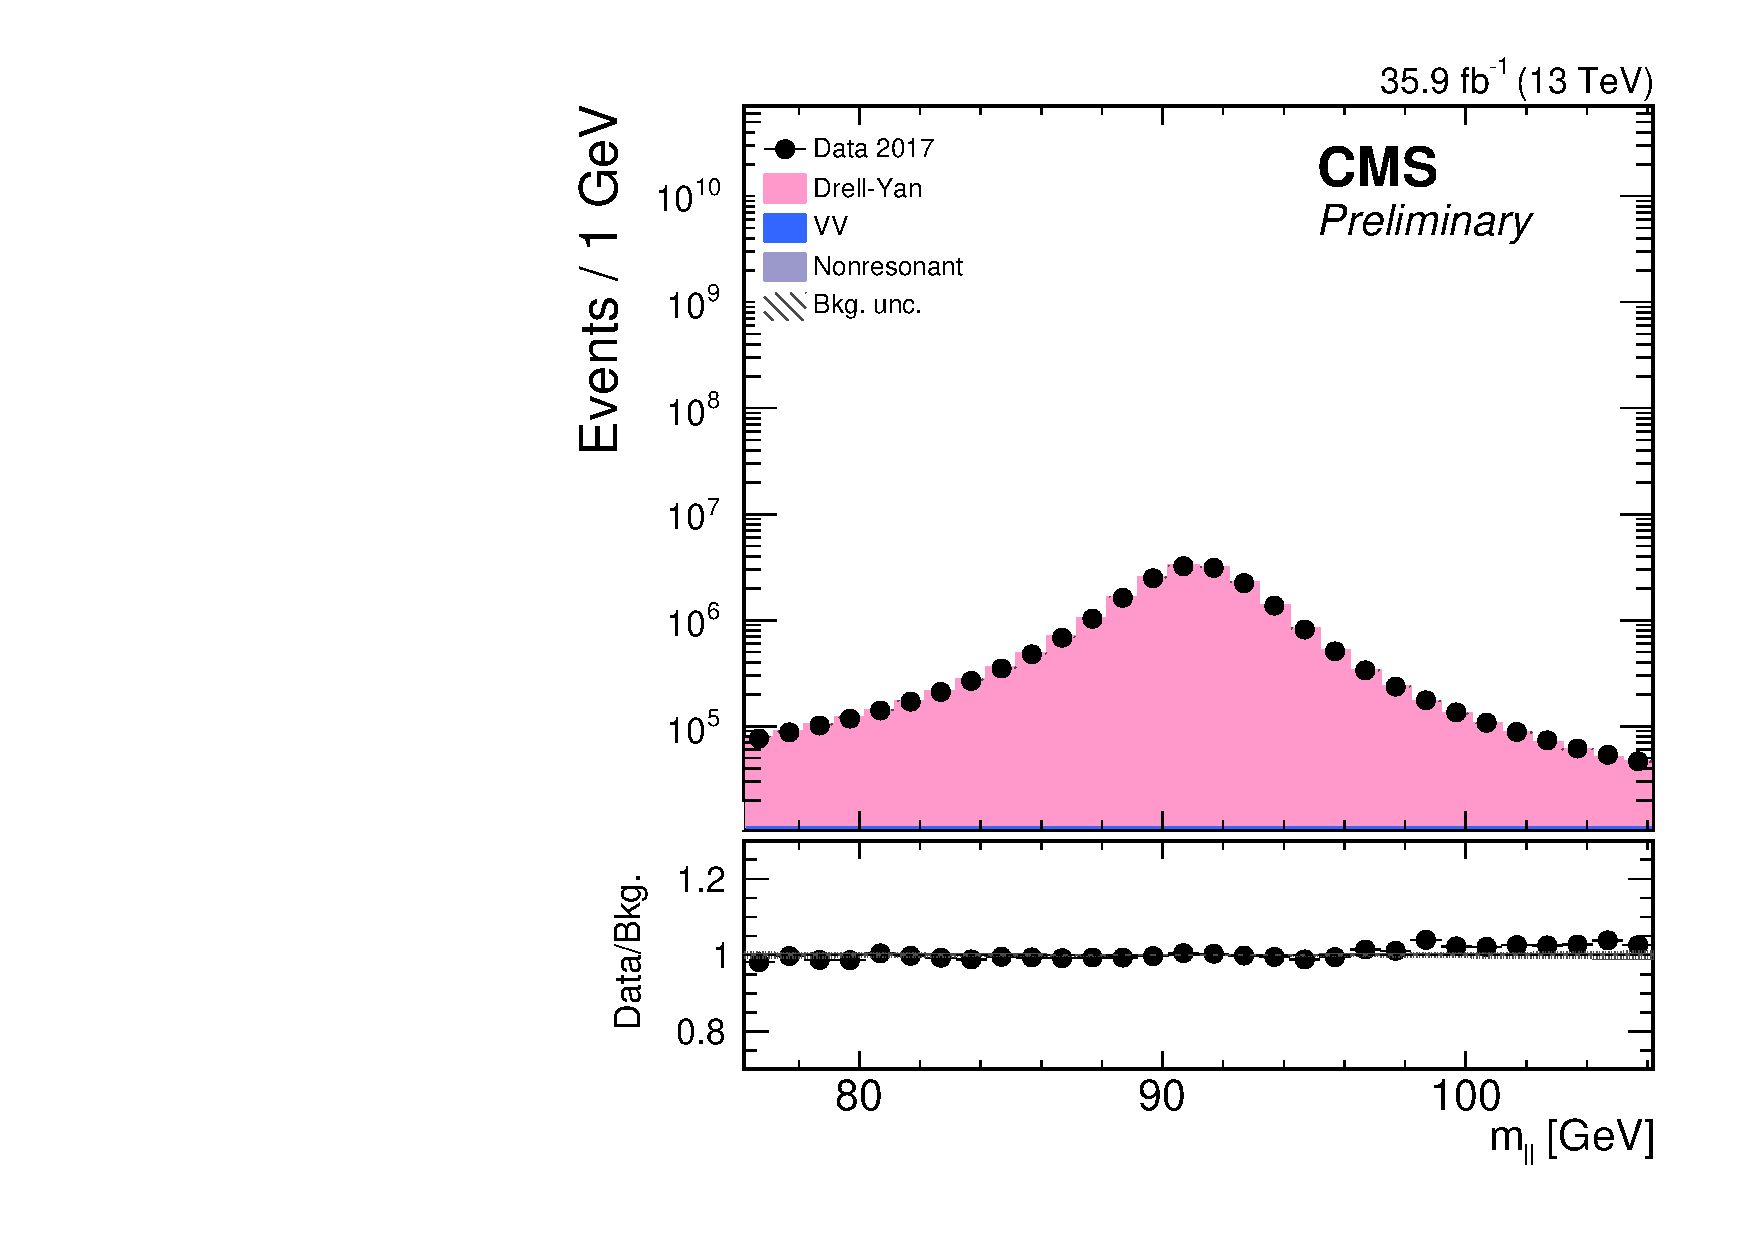
\includegraphics[width=0.49\textwidth]{figures/zpt/zmm_mll.pdf}
	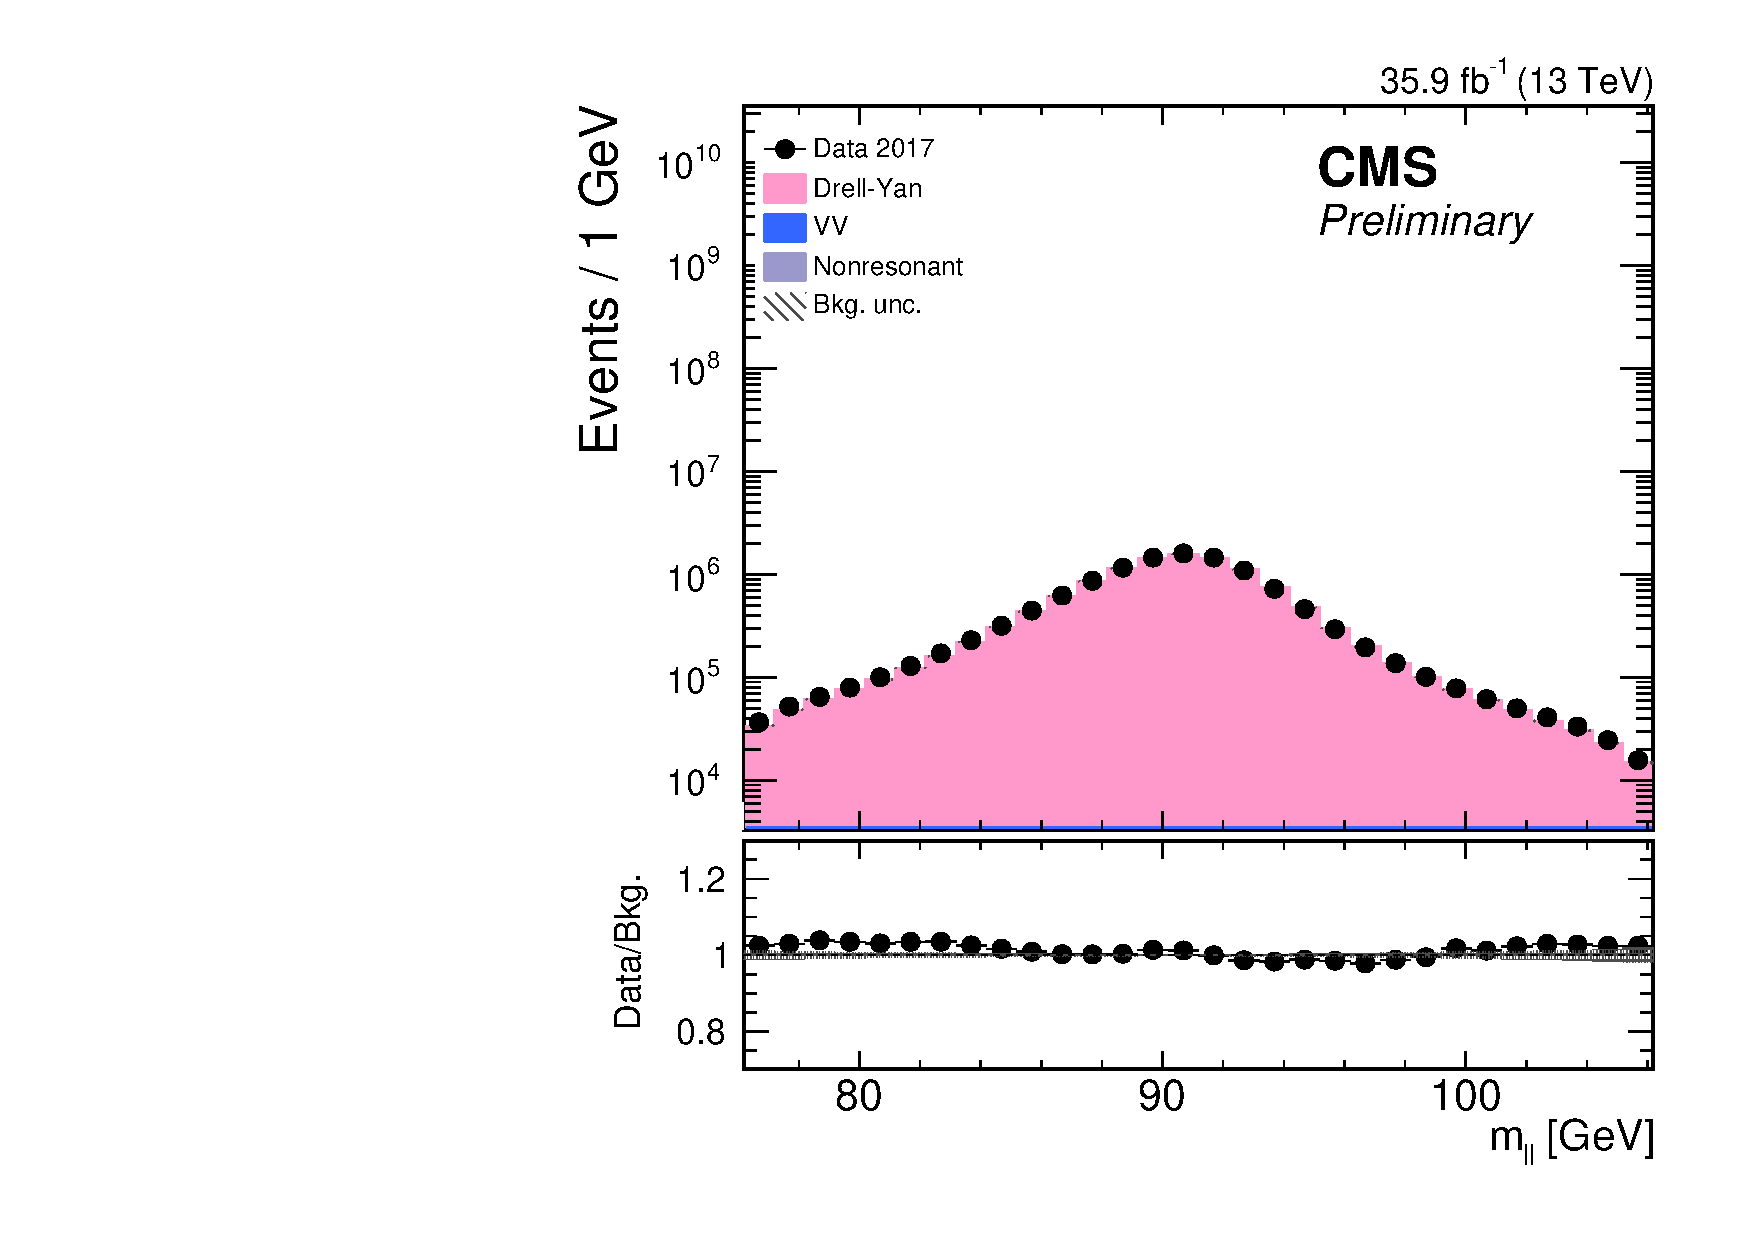
\includegraphics[width=0.49\textwidth]{figures/zpt/zee_mll.pdf}
	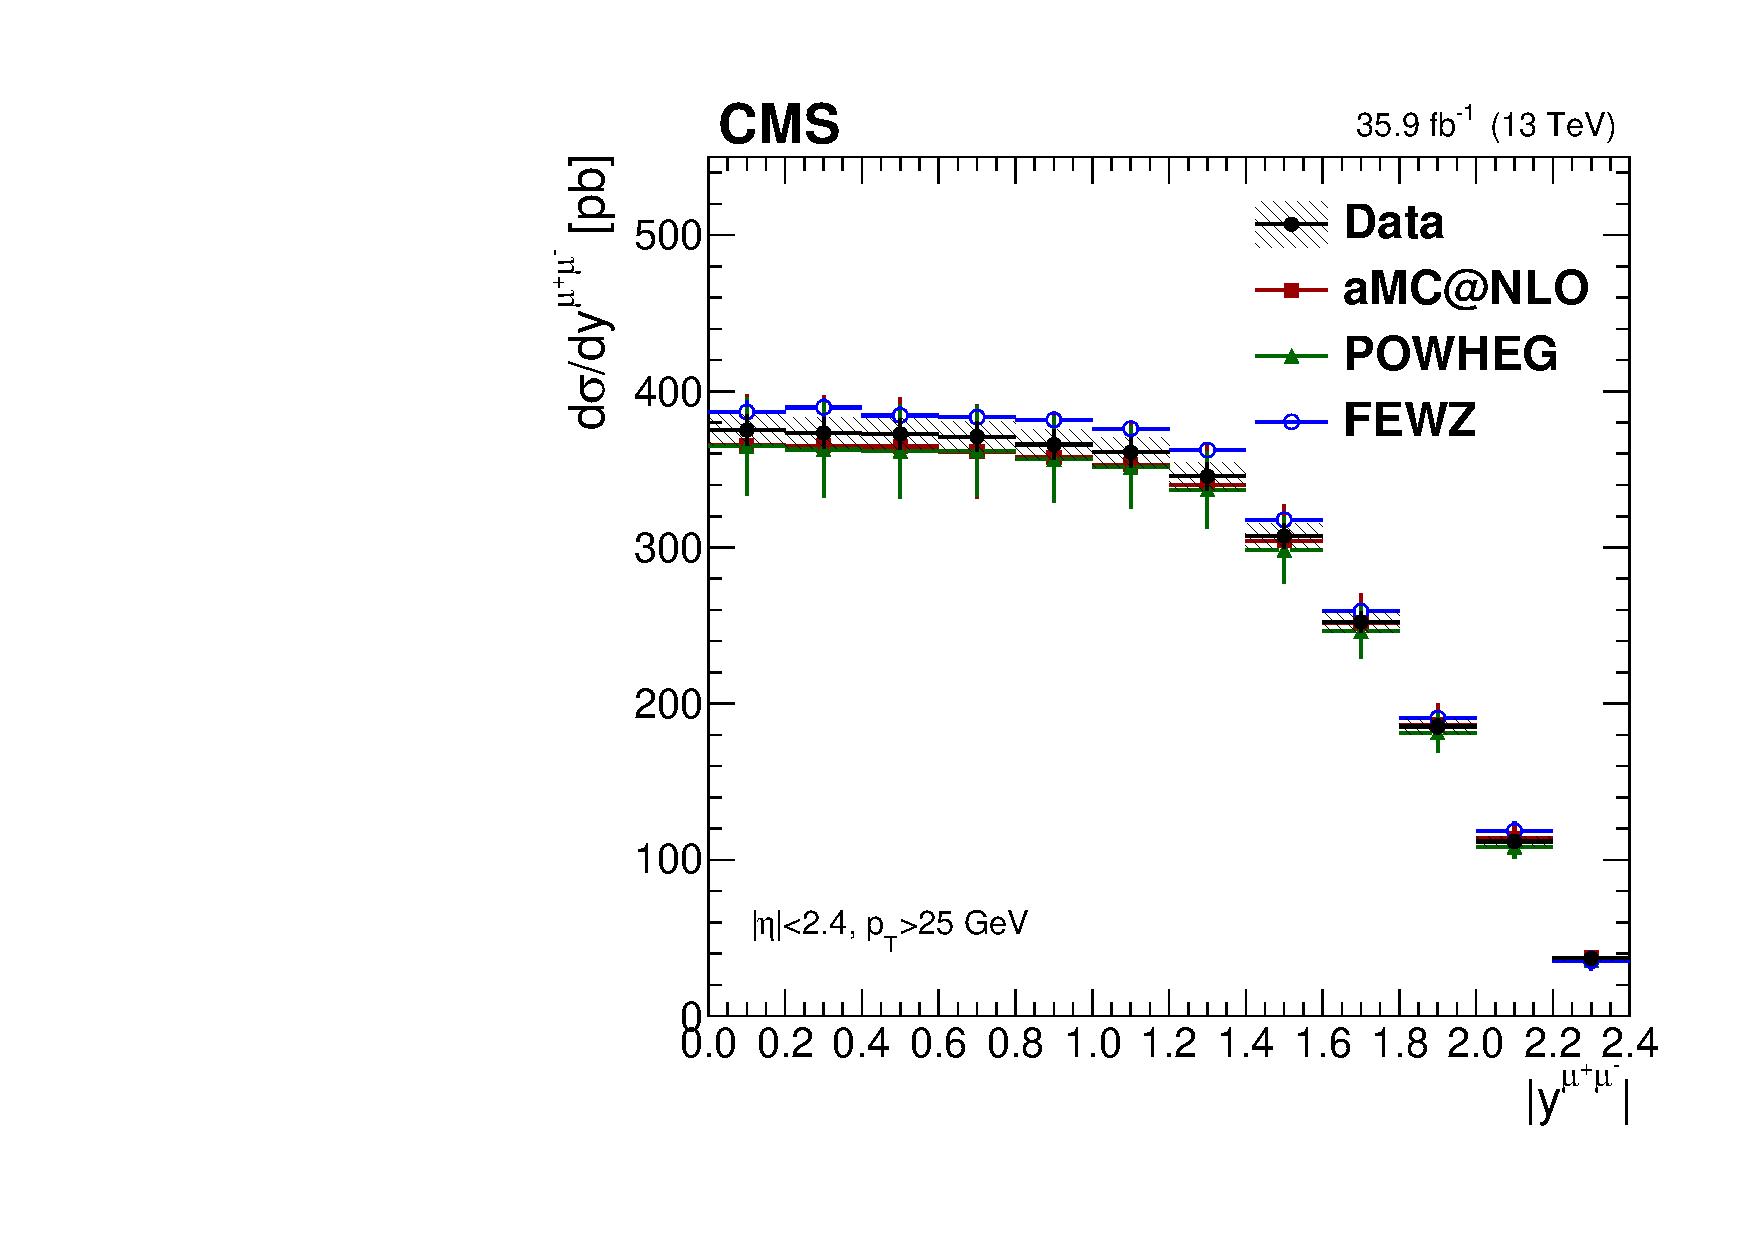
\includegraphics[width=0.49\textwidth]{figures/zpt/zmm_rap.pdf}
	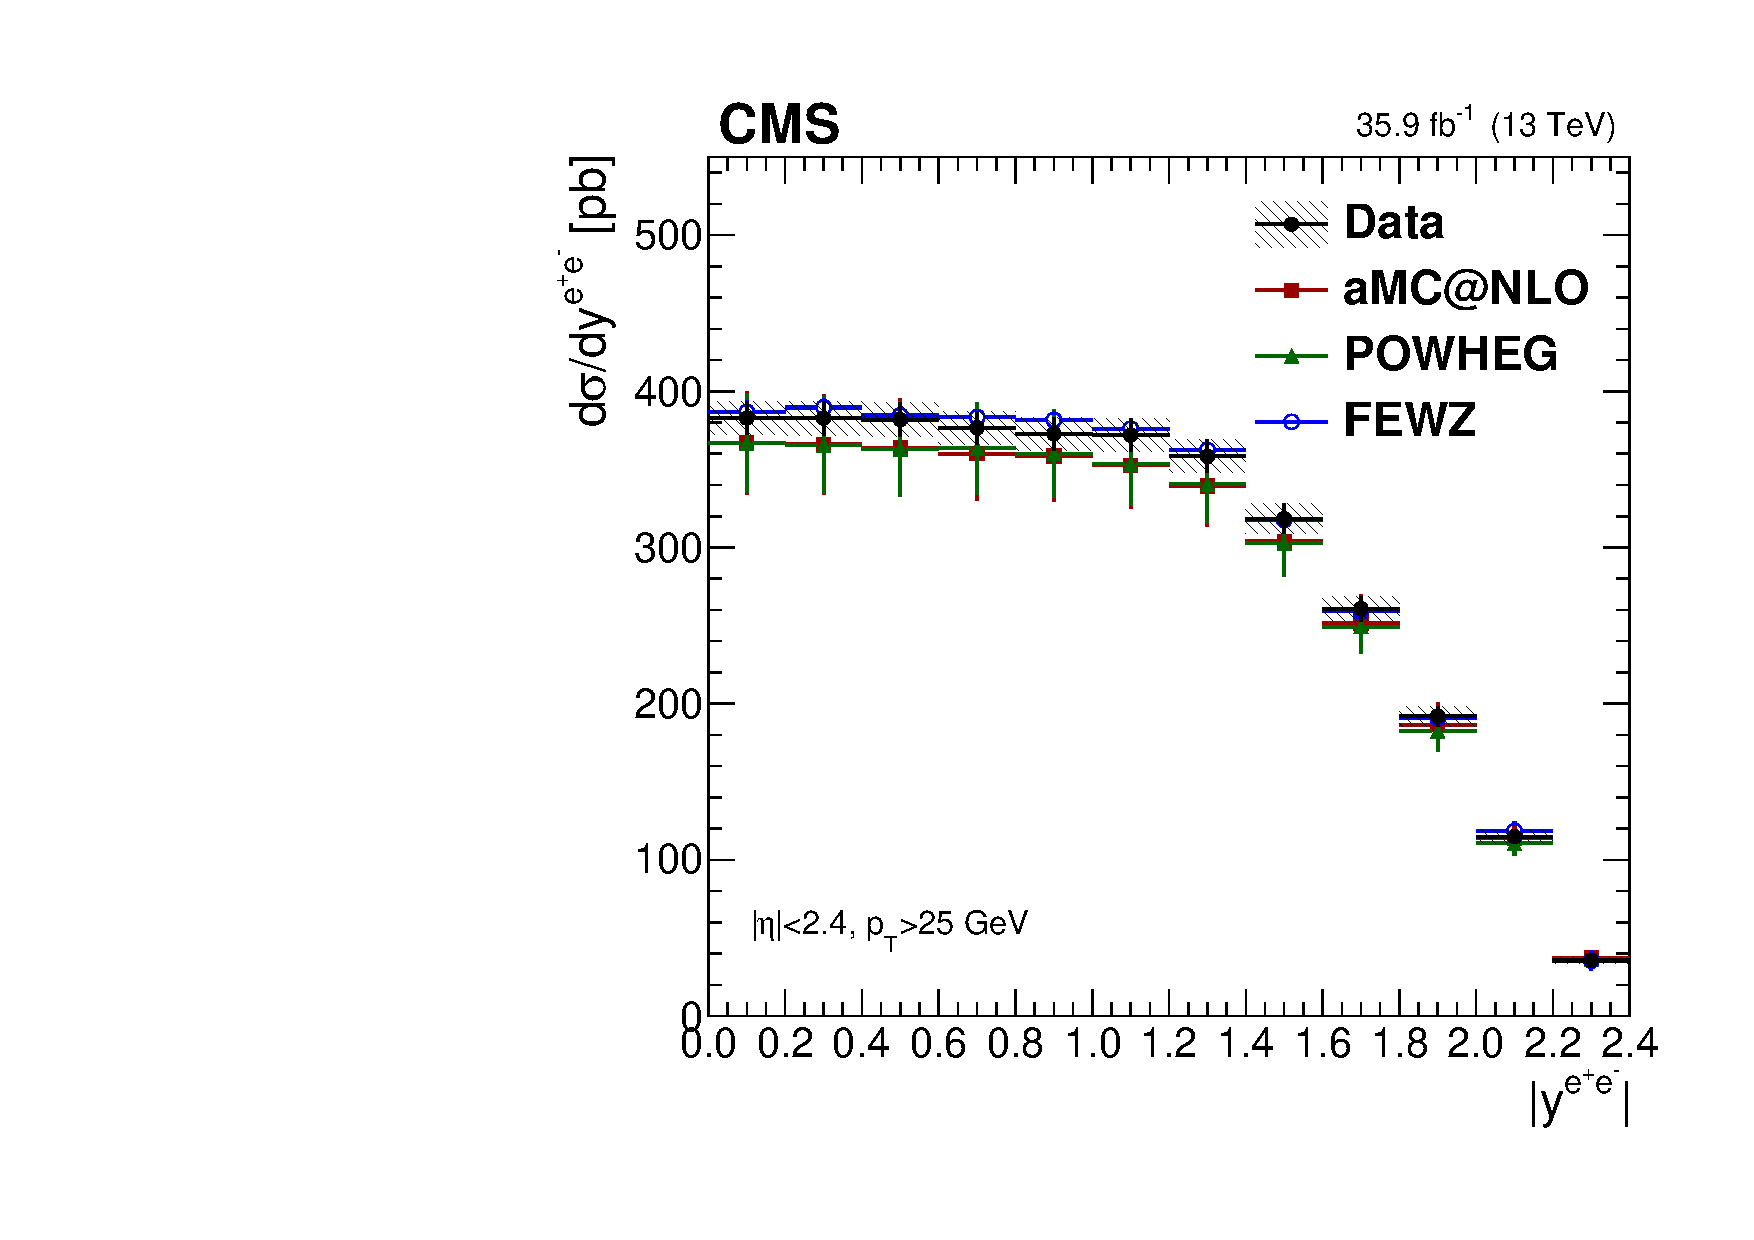
\includegraphics[width=0.49\textwidth]{figures/zpt/zee_rap.pdf}
	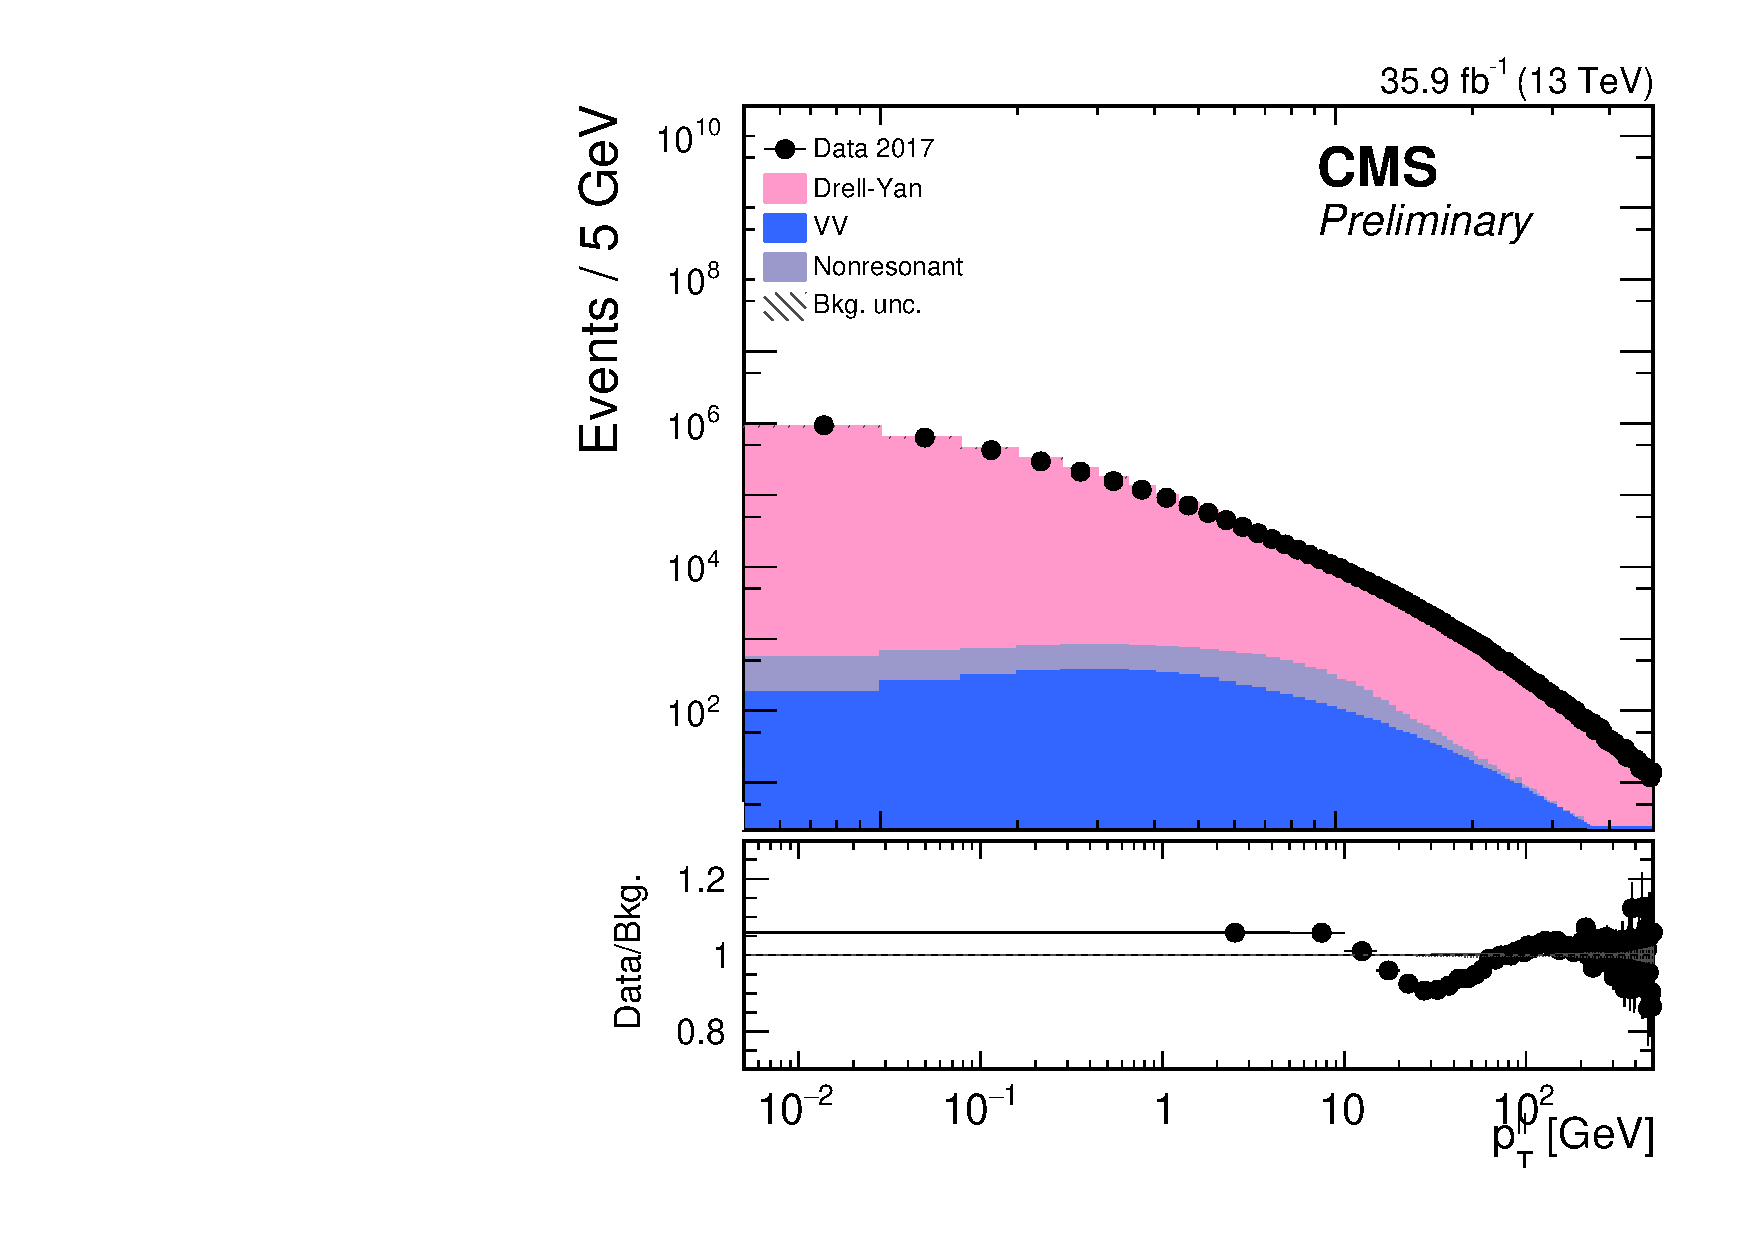
\includegraphics[width=0.49\textwidth]{figures/zpt/zmm_ptll.pdf}
	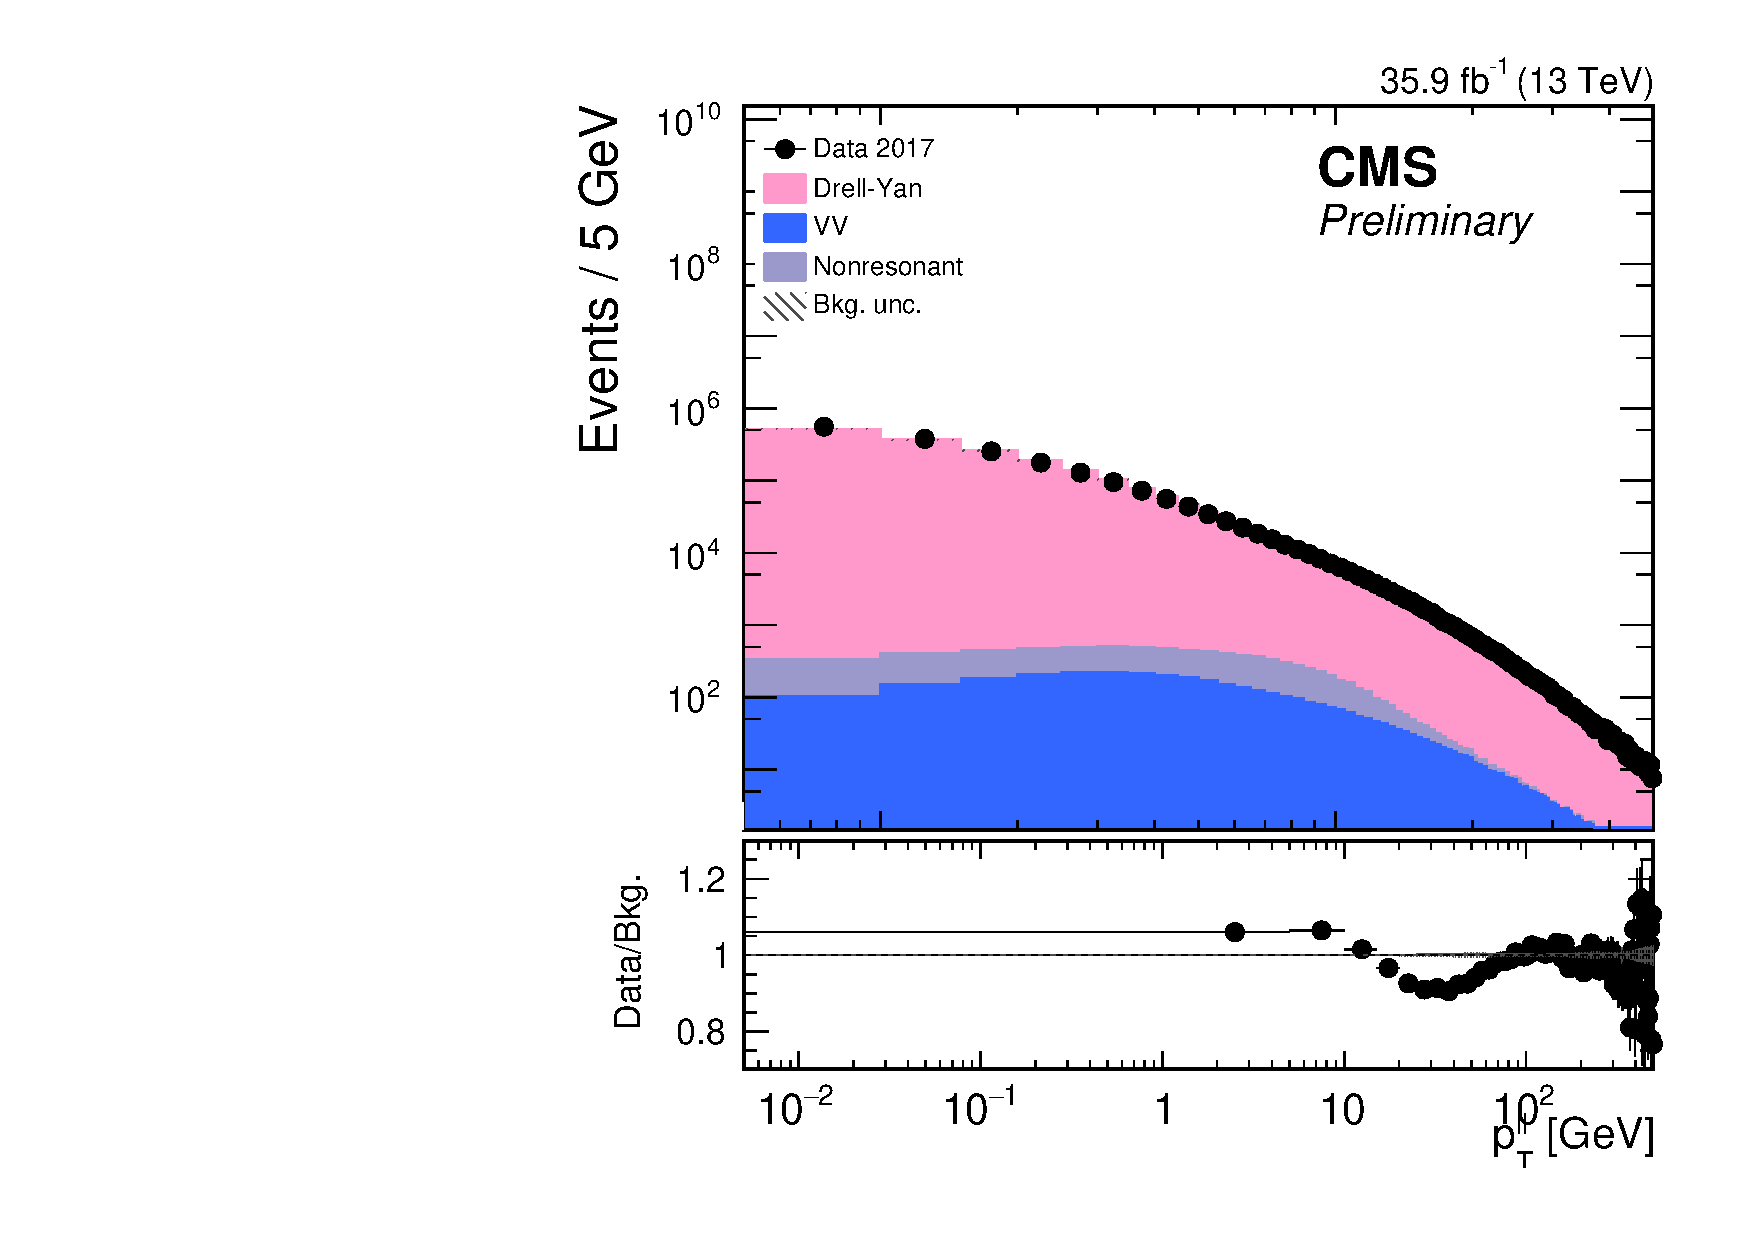
\includegraphics[width=0.49\textwidth]{figures/zpt/zee_ptll.pdf}
	\caption{Distributions at the reconstruction level of $\mll$ (top), $|\rapidity^\Z|$ (center), and 
	$\pt^\Z$ (bottom) for dimuons (left) and dielectrons (right) after applying the full selection.}
	\label{fig:recodist1}
\end{figure}

\begin{figure}
	\centering
	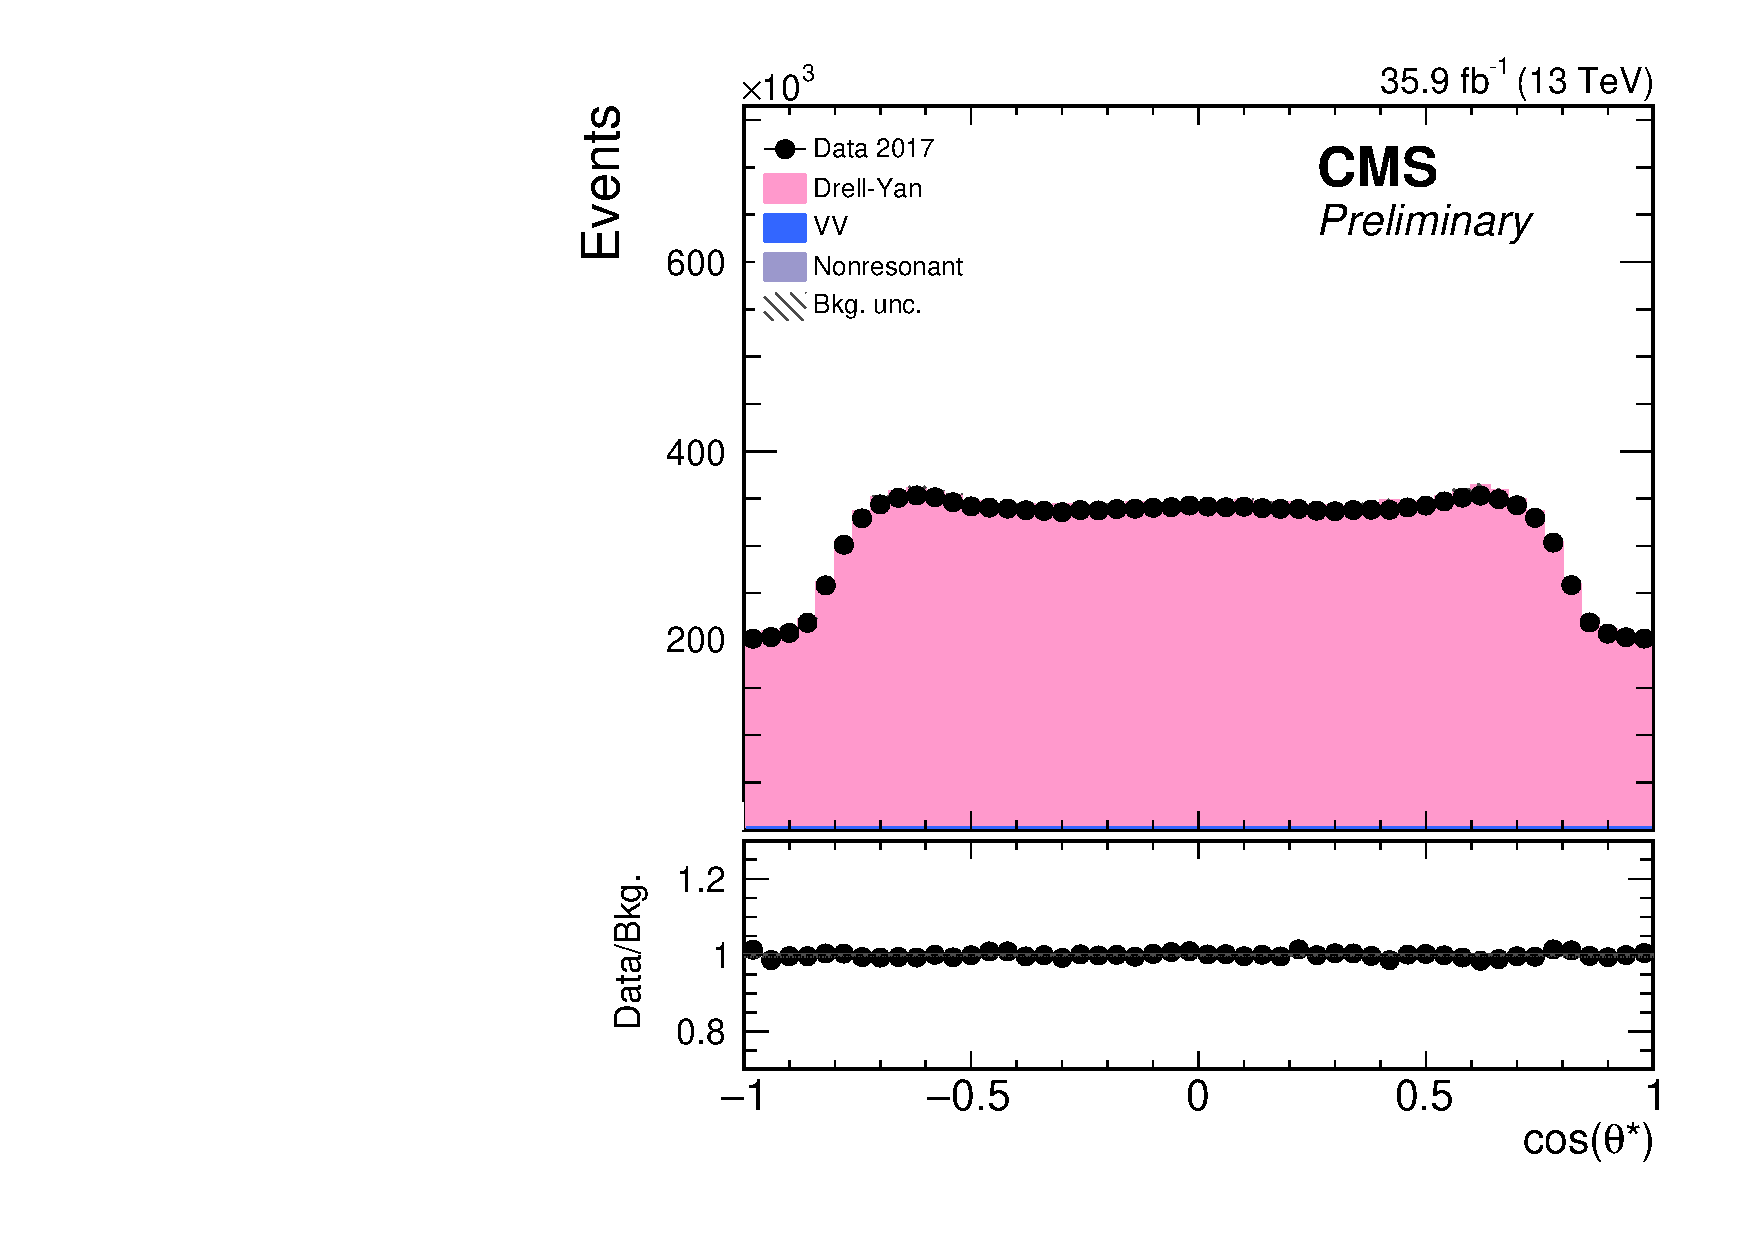
\includegraphics[width=0.49\textwidth]{figures/zpt/zmm_cos_theta_star.pdf}
	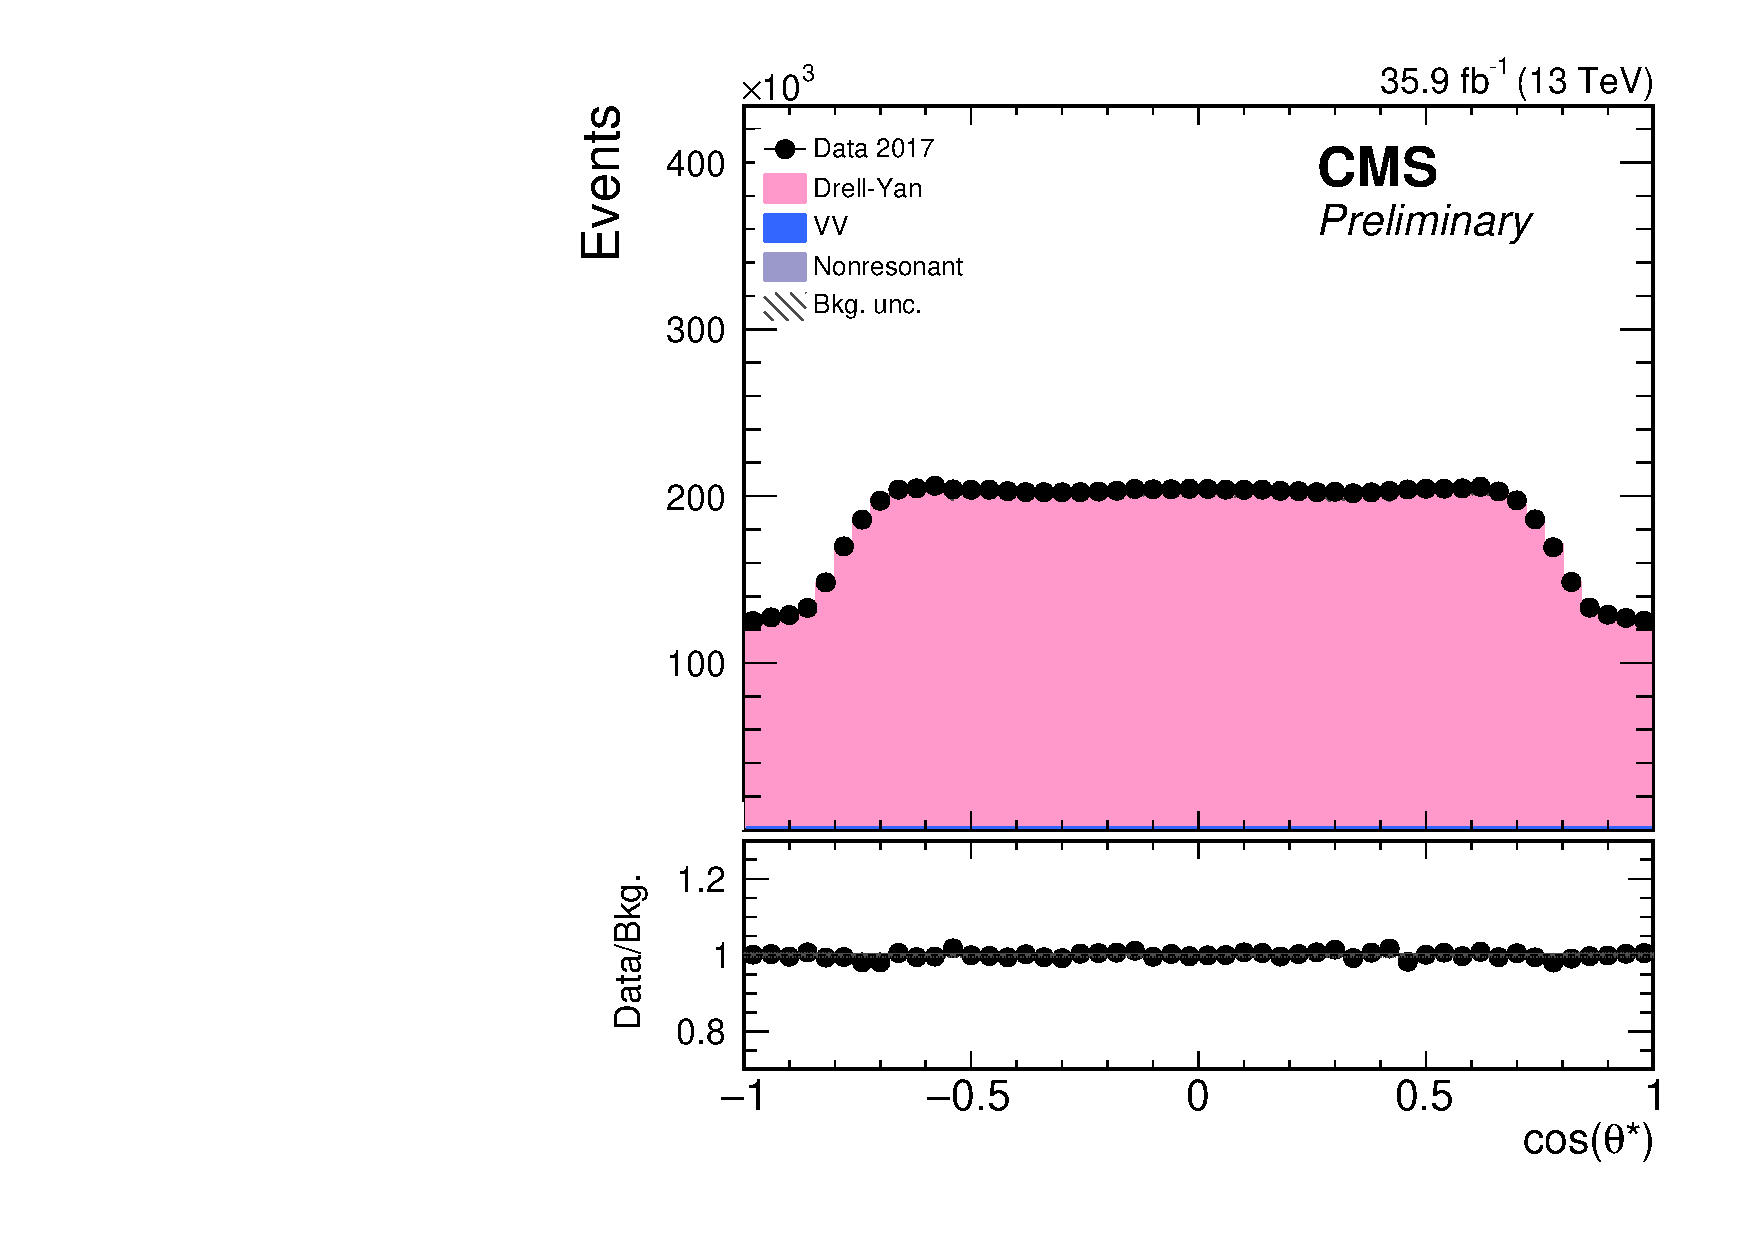
\includegraphics[width=0.49\textwidth]{figures/zpt/zee_cos_theta_star.pdf}
	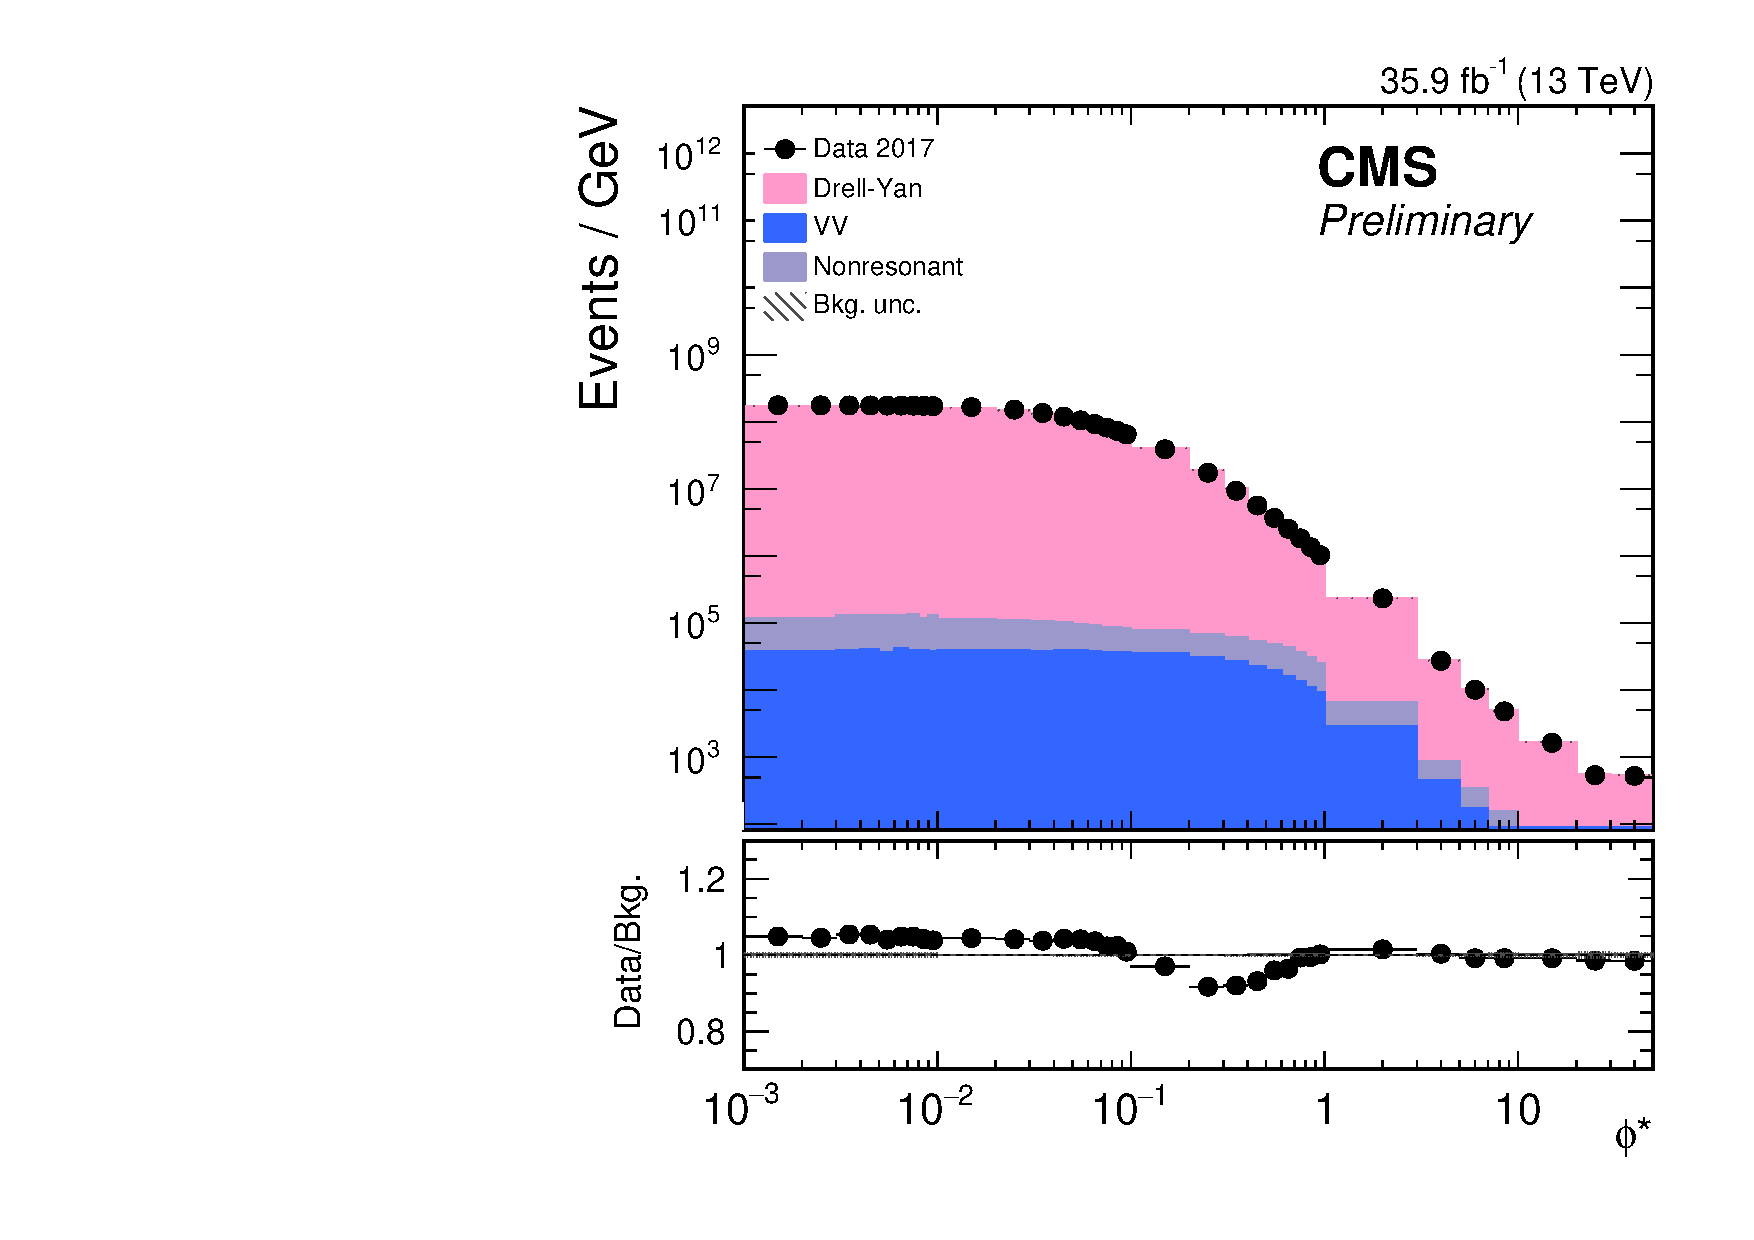
\includegraphics[width=0.49\textwidth]{figures/zpt/zmm_phi_star.pdf}
	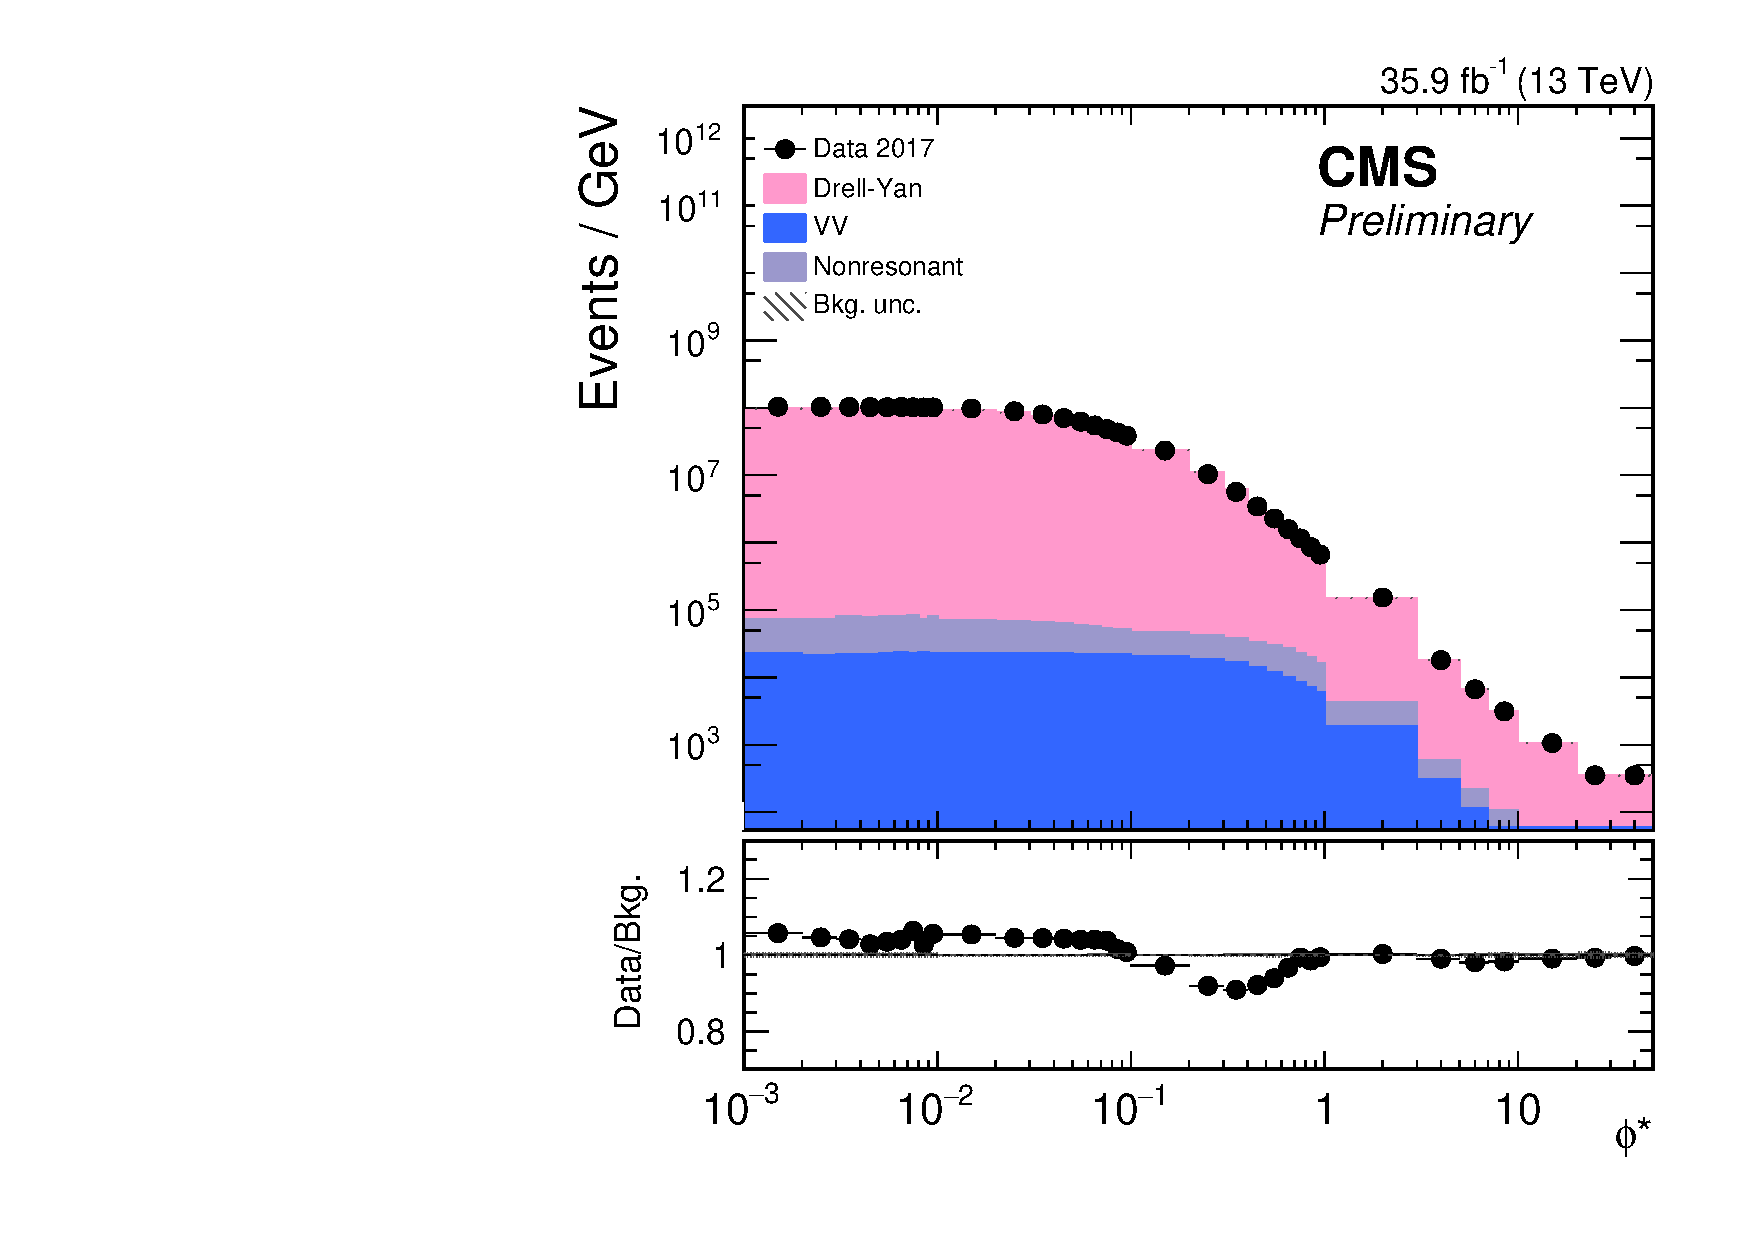
\includegraphics[width=0.49\textwidth]{figures/zpt/zee_phi_star.pdf}
	\caption{Distributions at the reconstruction level of $cos(\theta^\star$ (top) and $\phi^\star$ (bottom) for dimuons 
	(left) and dielectrons (right) after applying the full selection.}
	\label{fig:recodist2}
\end{figure}

\begin{figure}
	\centering
	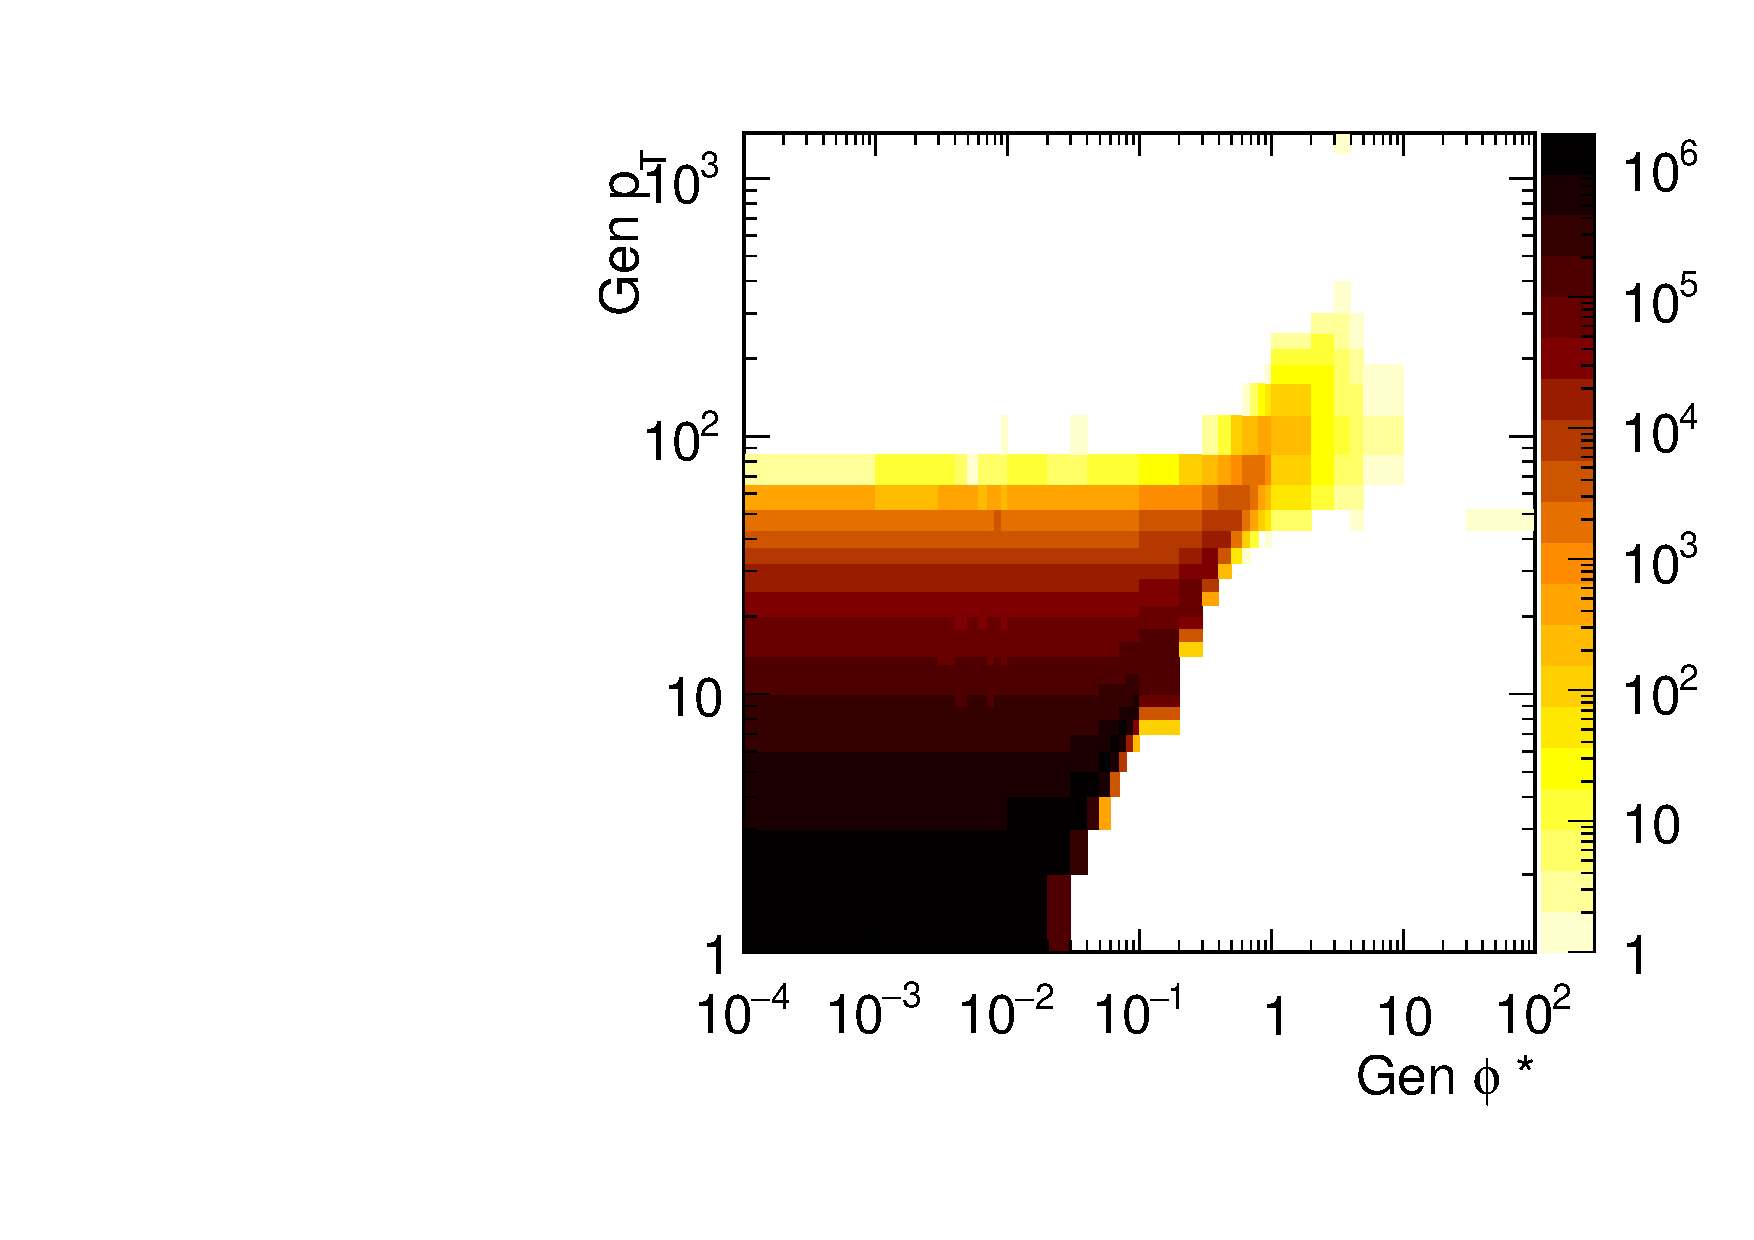
\includegraphics[width=0.49\textwidth]{figures/zpt/phiVpt.pdf}
	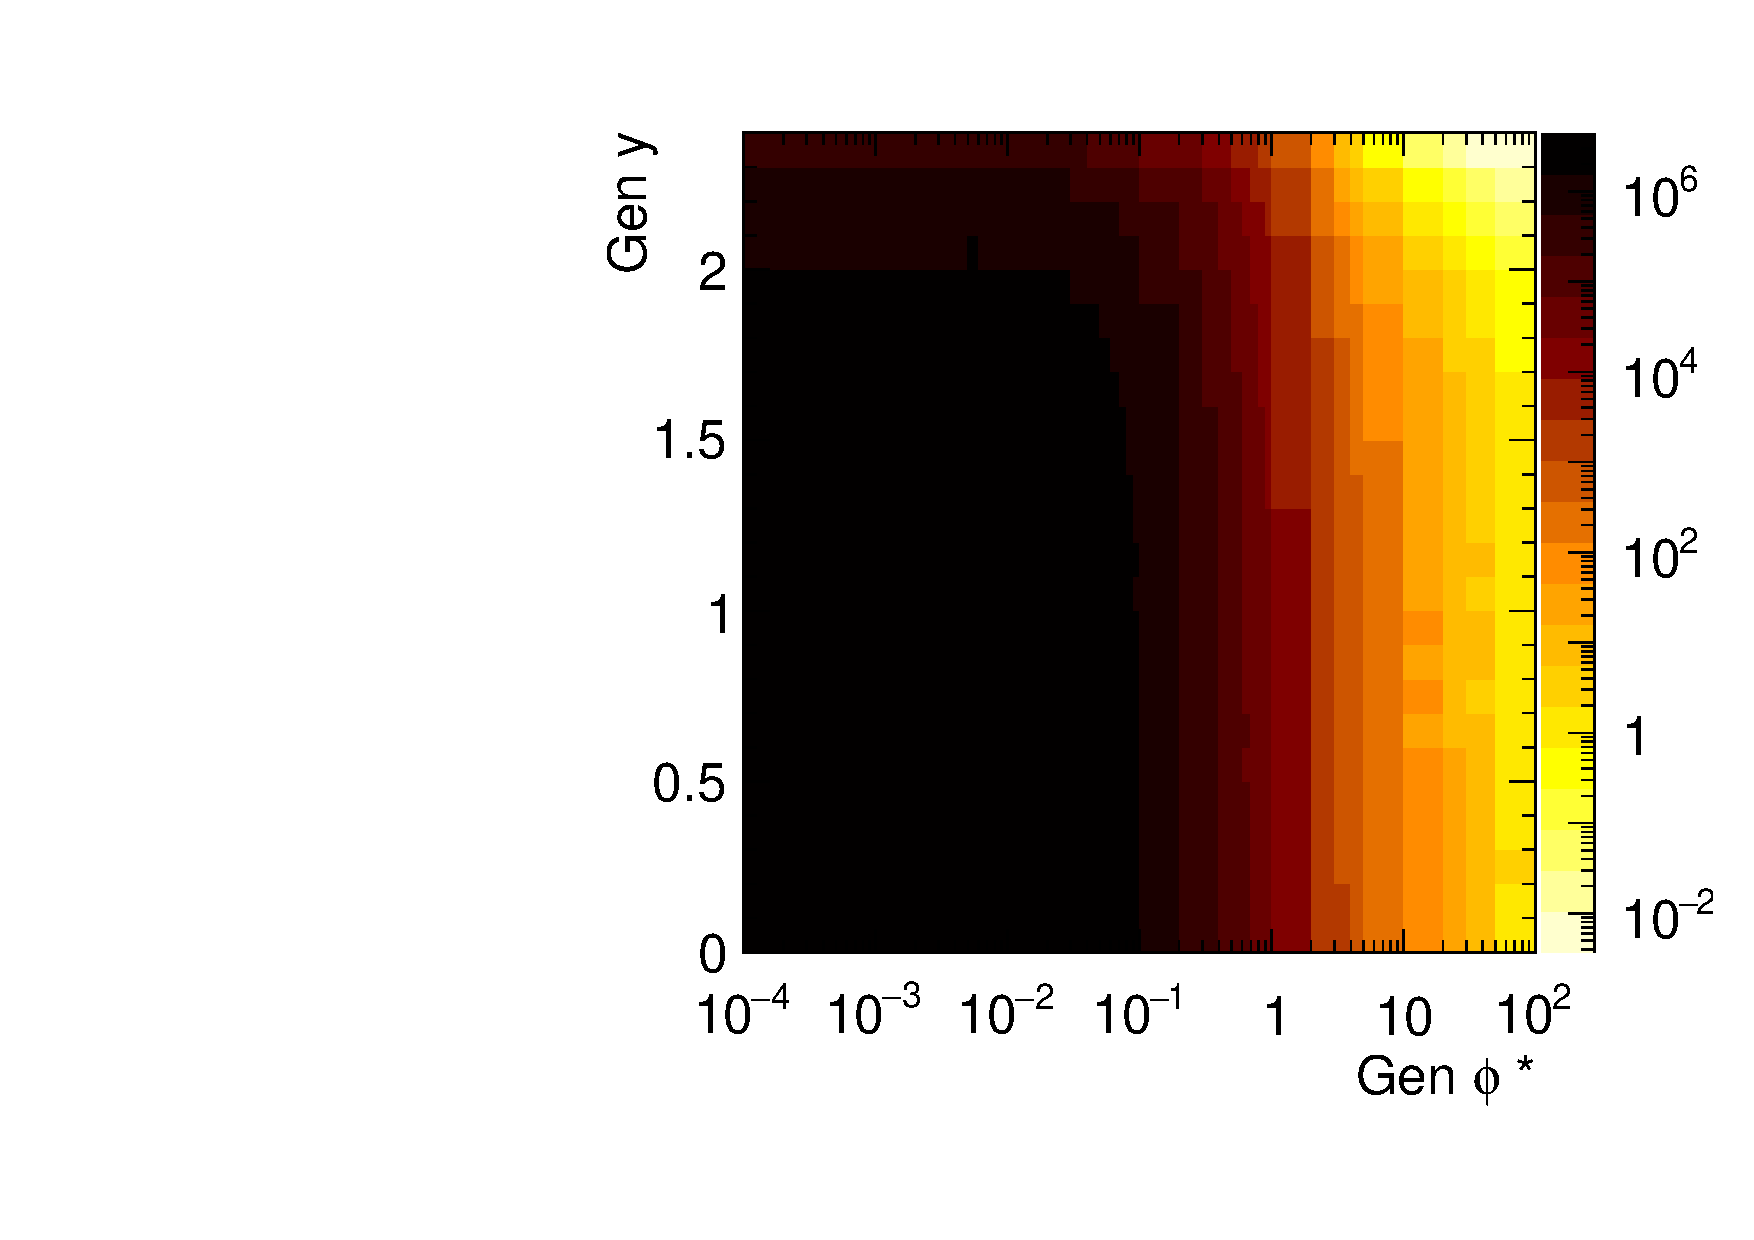
\includegraphics[width=0.49\textwidth]{figures/zpt/phiVrap.pdf}
	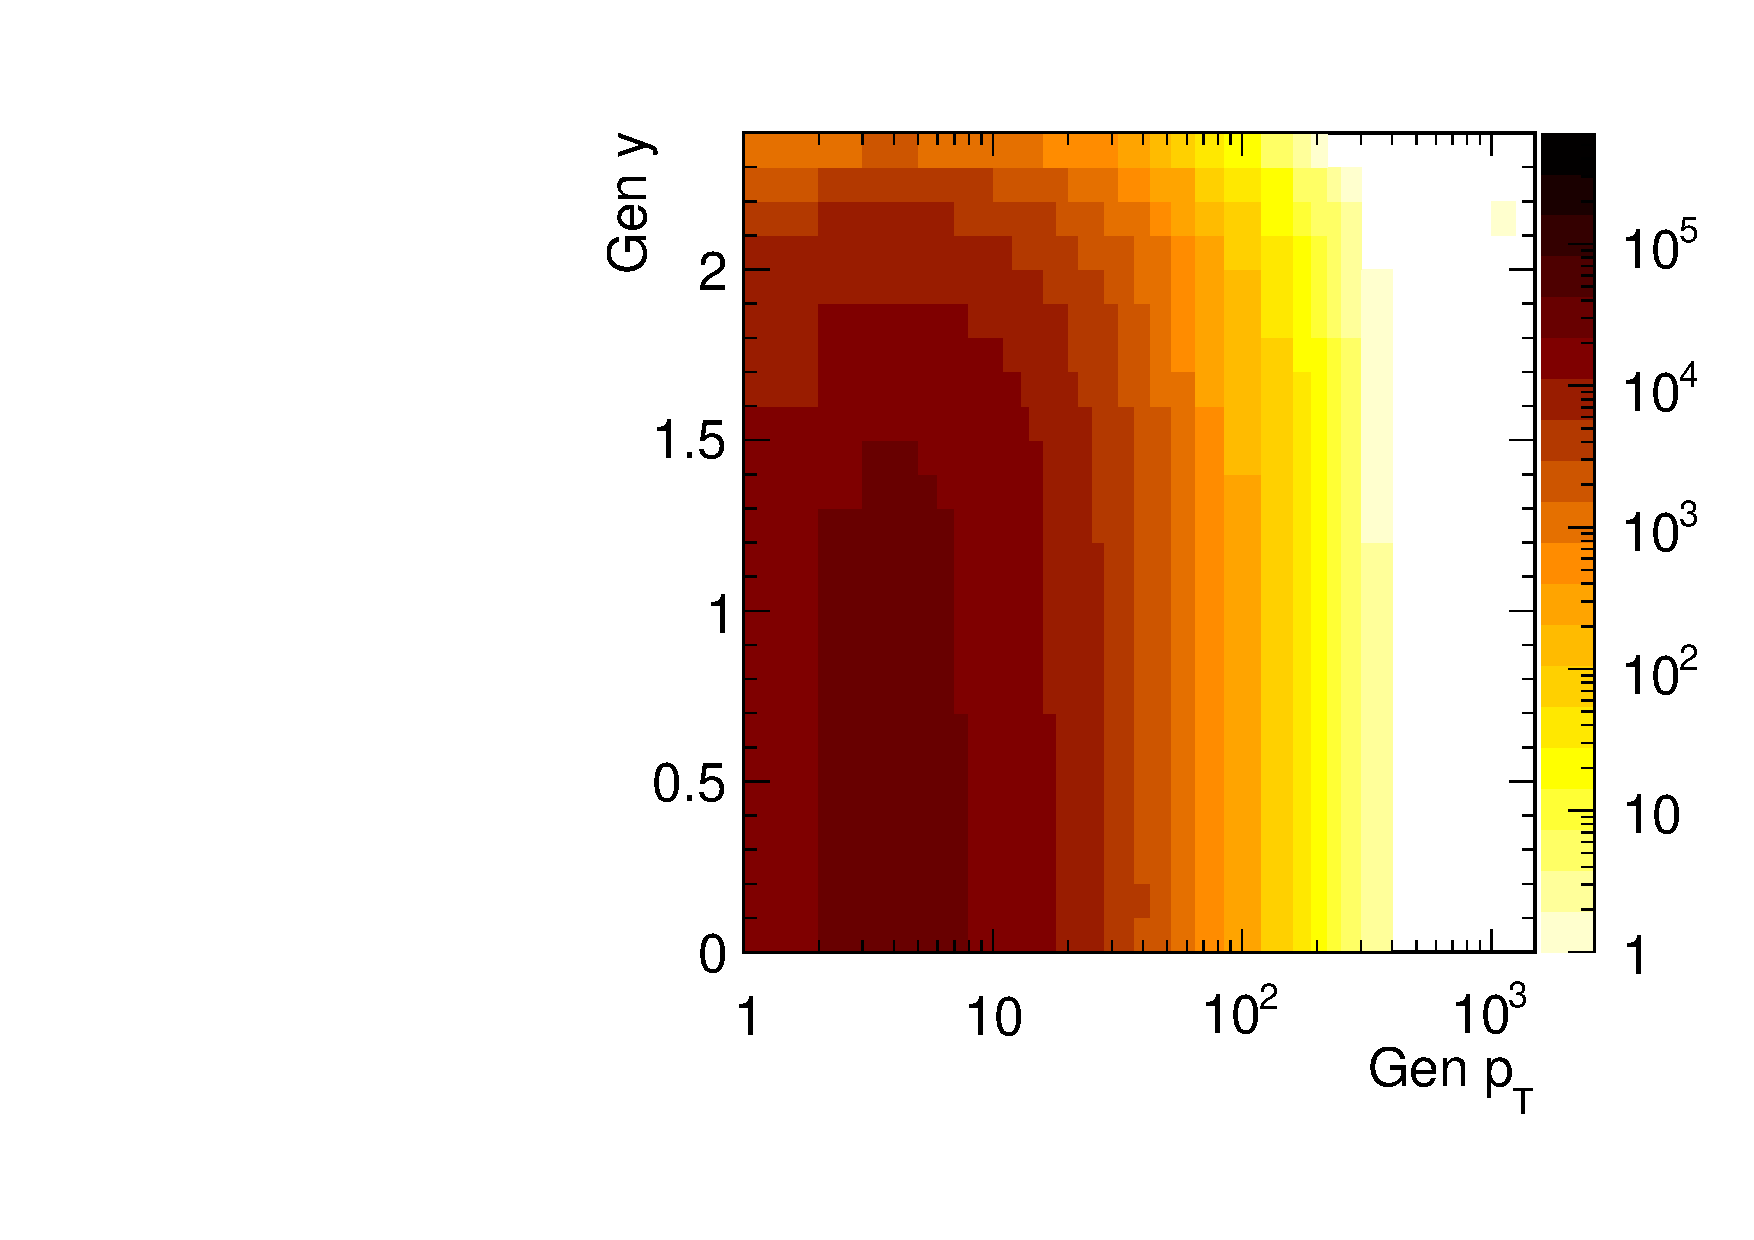
\includegraphics[width=0.49\textwidth]{figures/zpt/ptVrap.pdf}
	\caption{Distributions at the generator level of $\phi^\star$ vs $\pt^\Z$ (top left), $\phi^\star$ vs $y^\Z$ (top right), and $\pt^\Z$ vs $y^\Z$ (bottom) for dilepton pairs.}
	\label{fig:gendist1}
\end{figure}

\begin{figure}
	\centering
	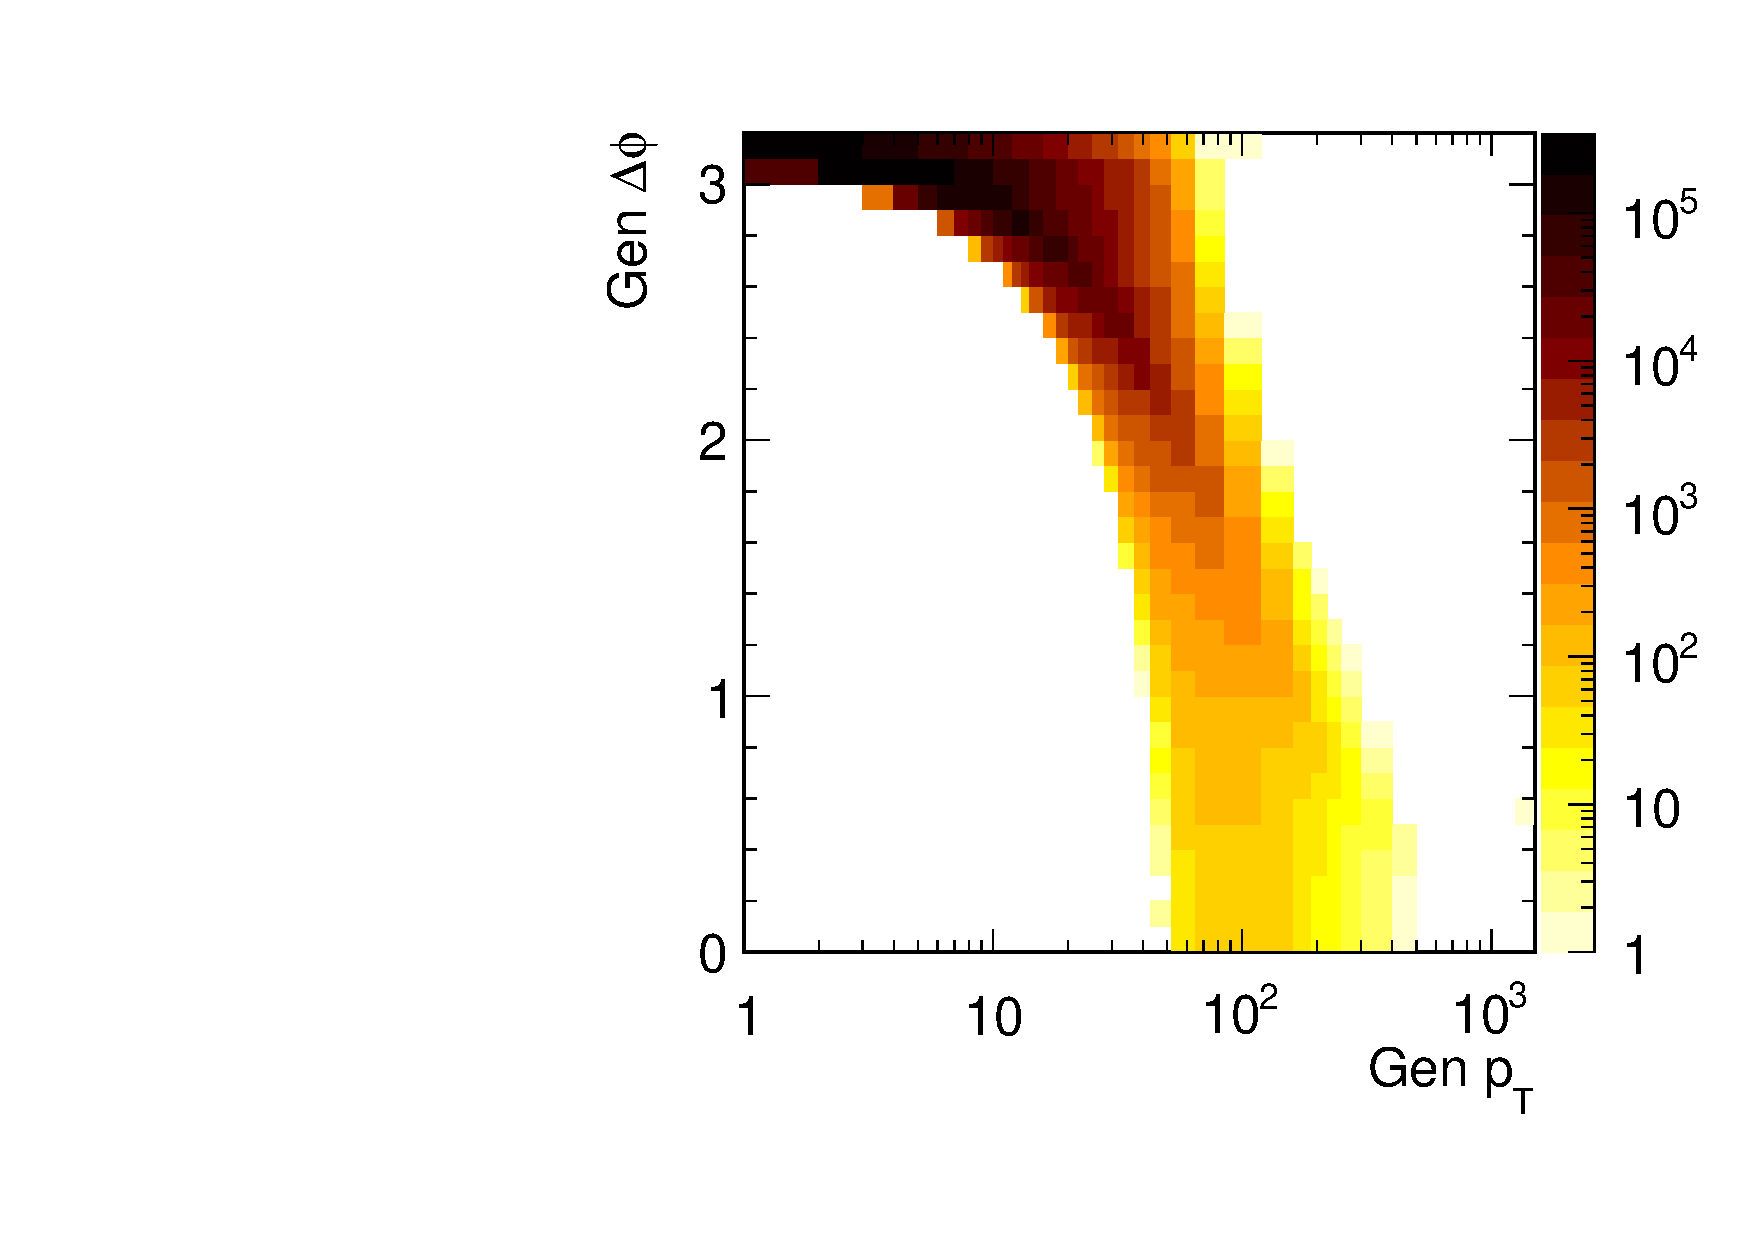
\includegraphics[width=0.49\textwidth]{figures/zpt/ptVdphi.pdf}
	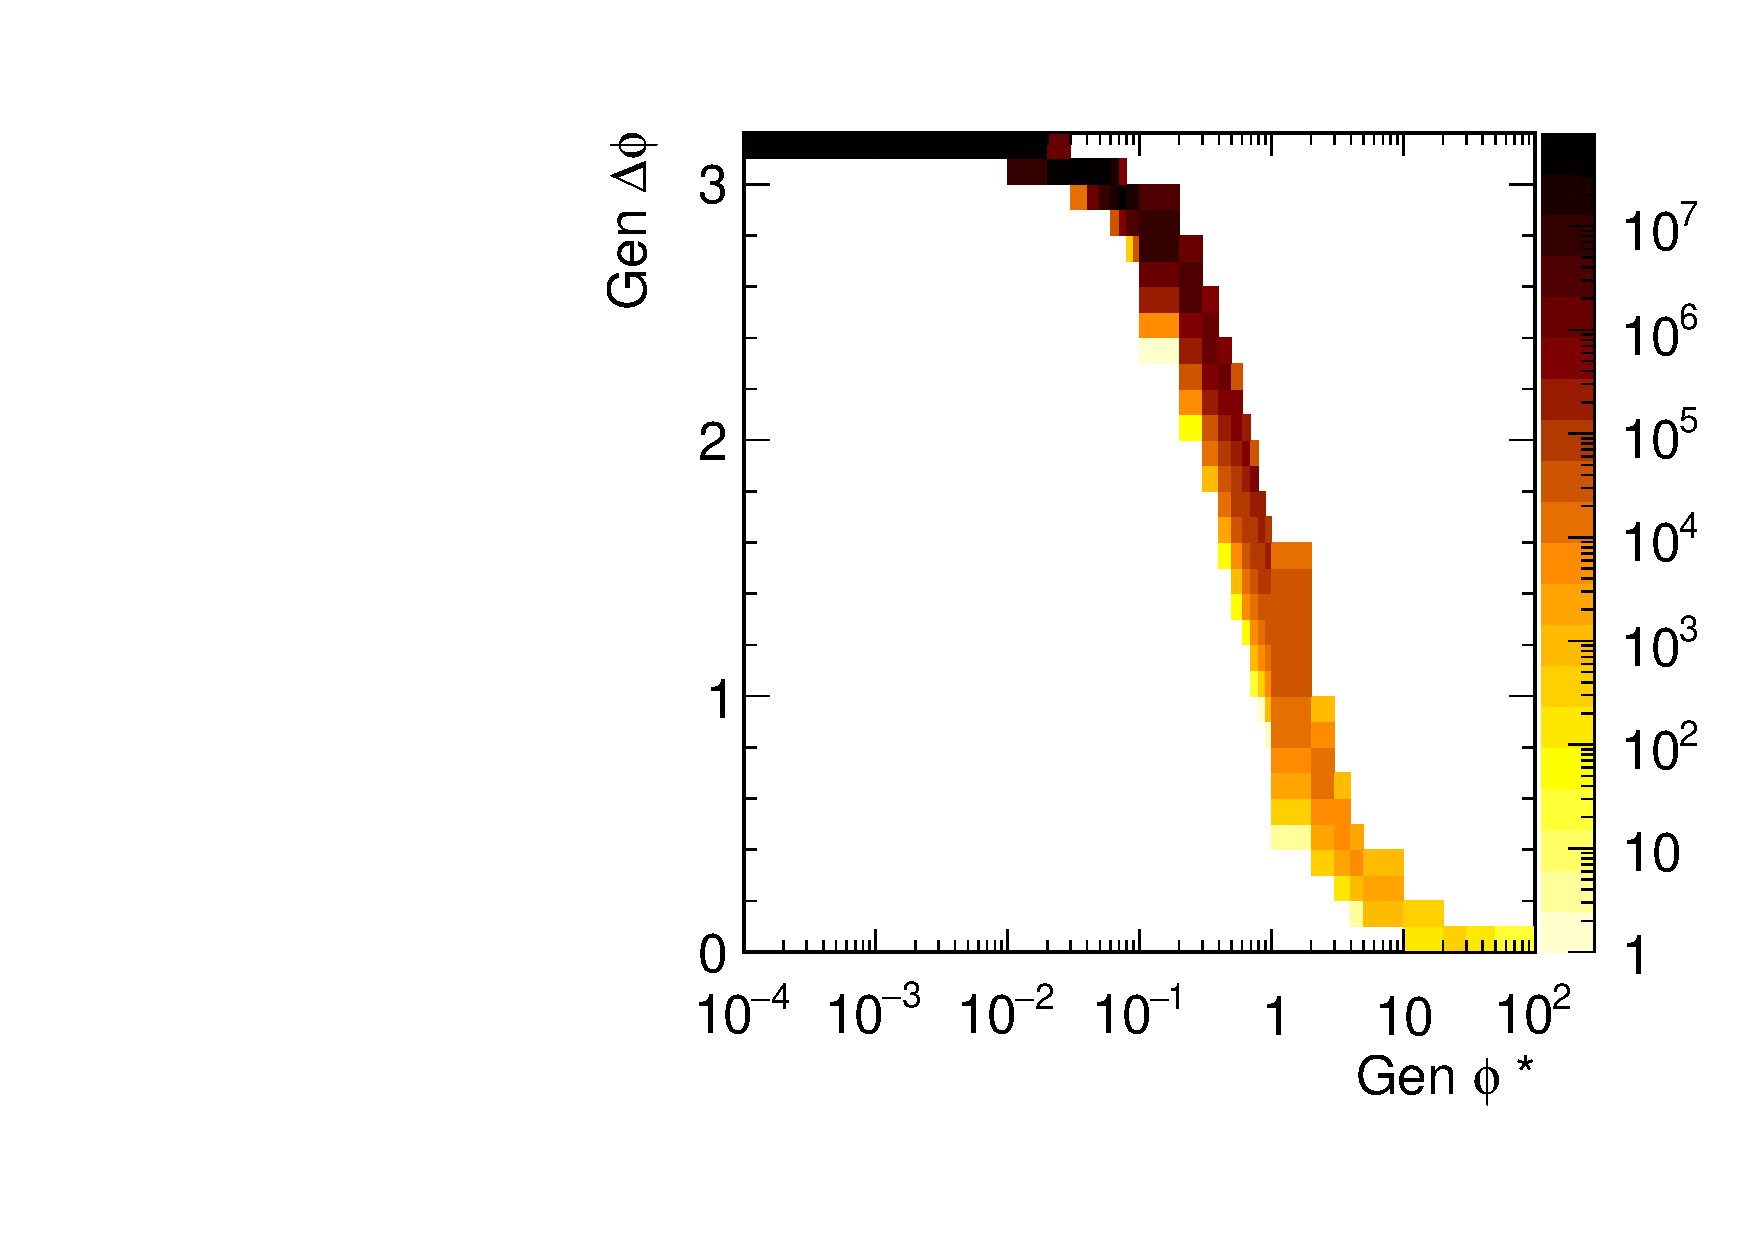
\includegraphics[width=0.49\textwidth]{figures/zpt/phiVdphi.pdf}
	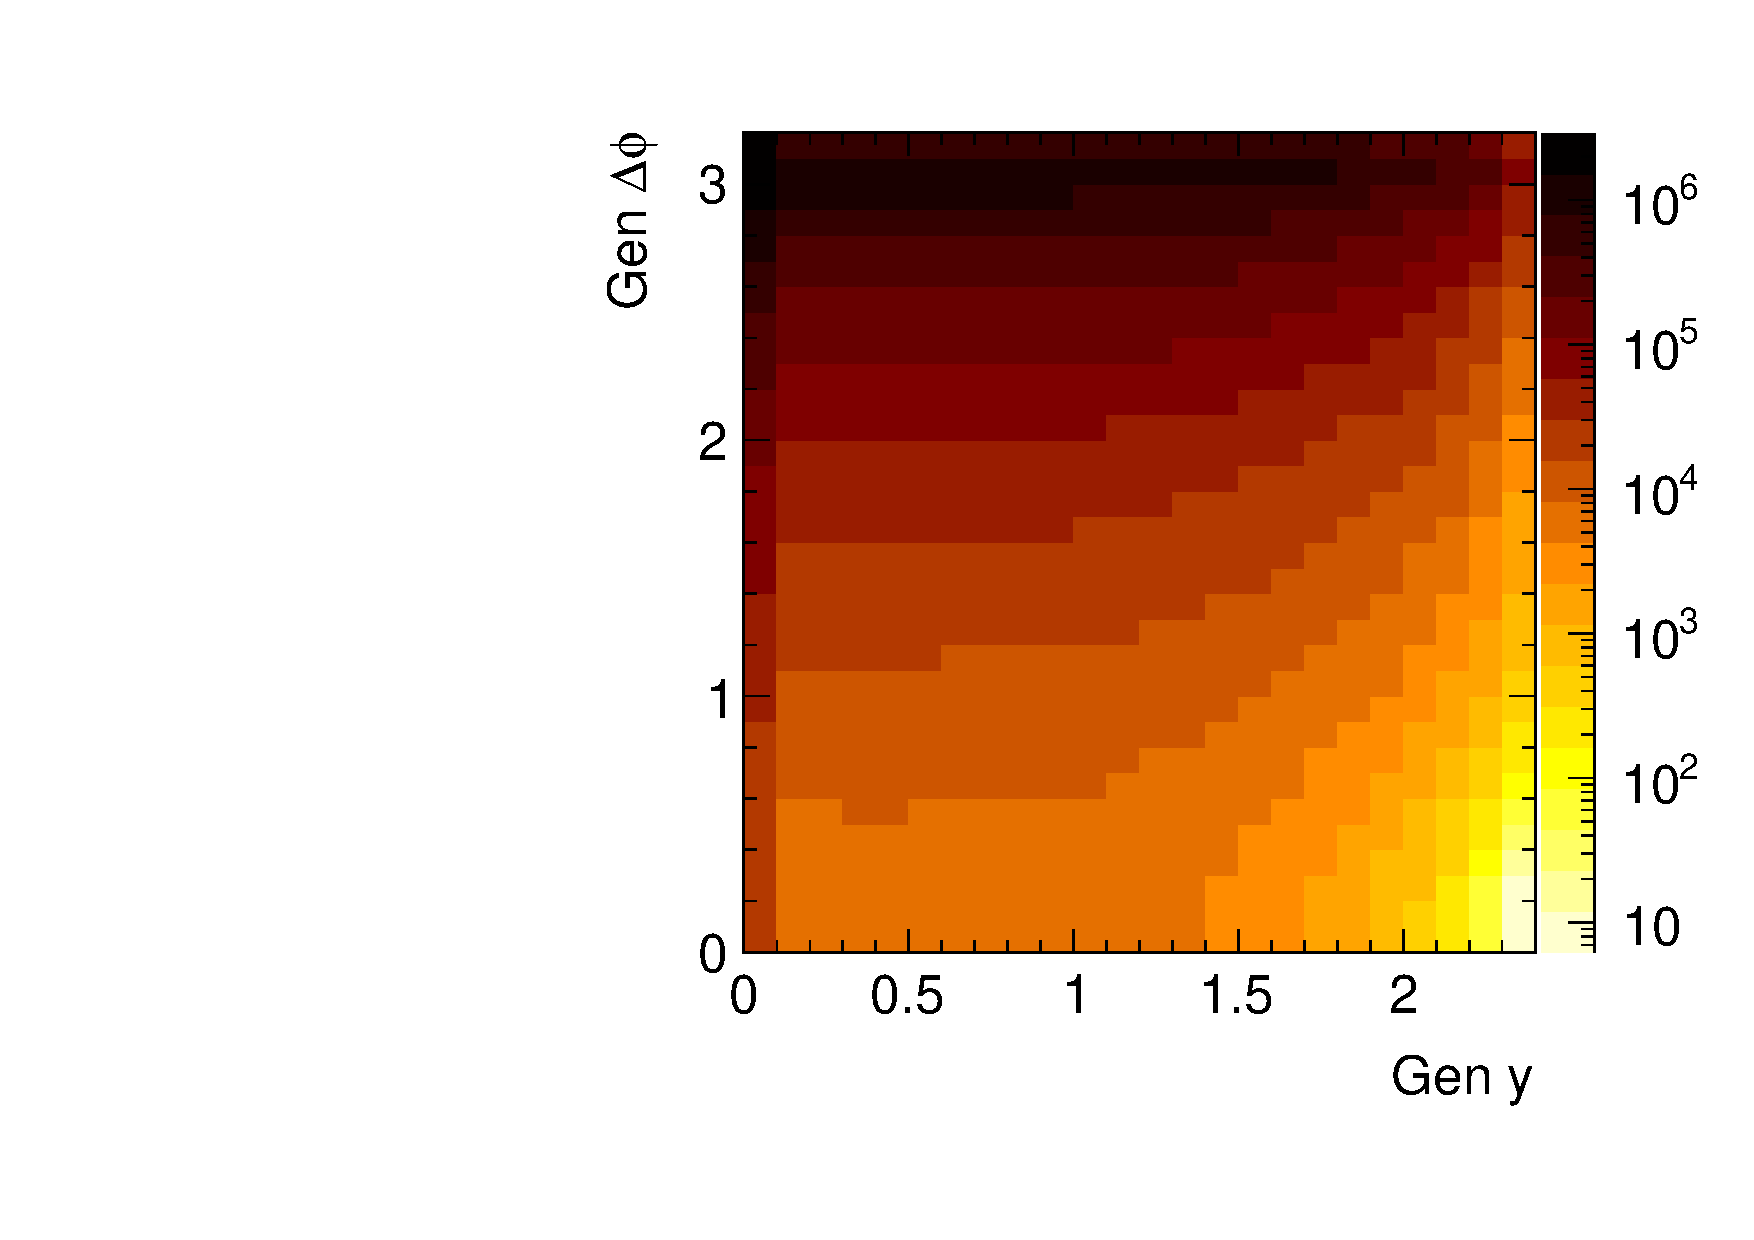
\includegraphics[width=0.49\textwidth]{figures/zpt/rapVdphi.pdf}
	\caption{Distributions at the generator level of $\Delta\phi$ with $\pt^\Z$ (top left), $\phi^\star$ (top right), and $y^\Z$ (bottom) for dilepton pairs.}
	\label{fig:gendist2}
\end{figure}

\begin{figure}
	\centering
	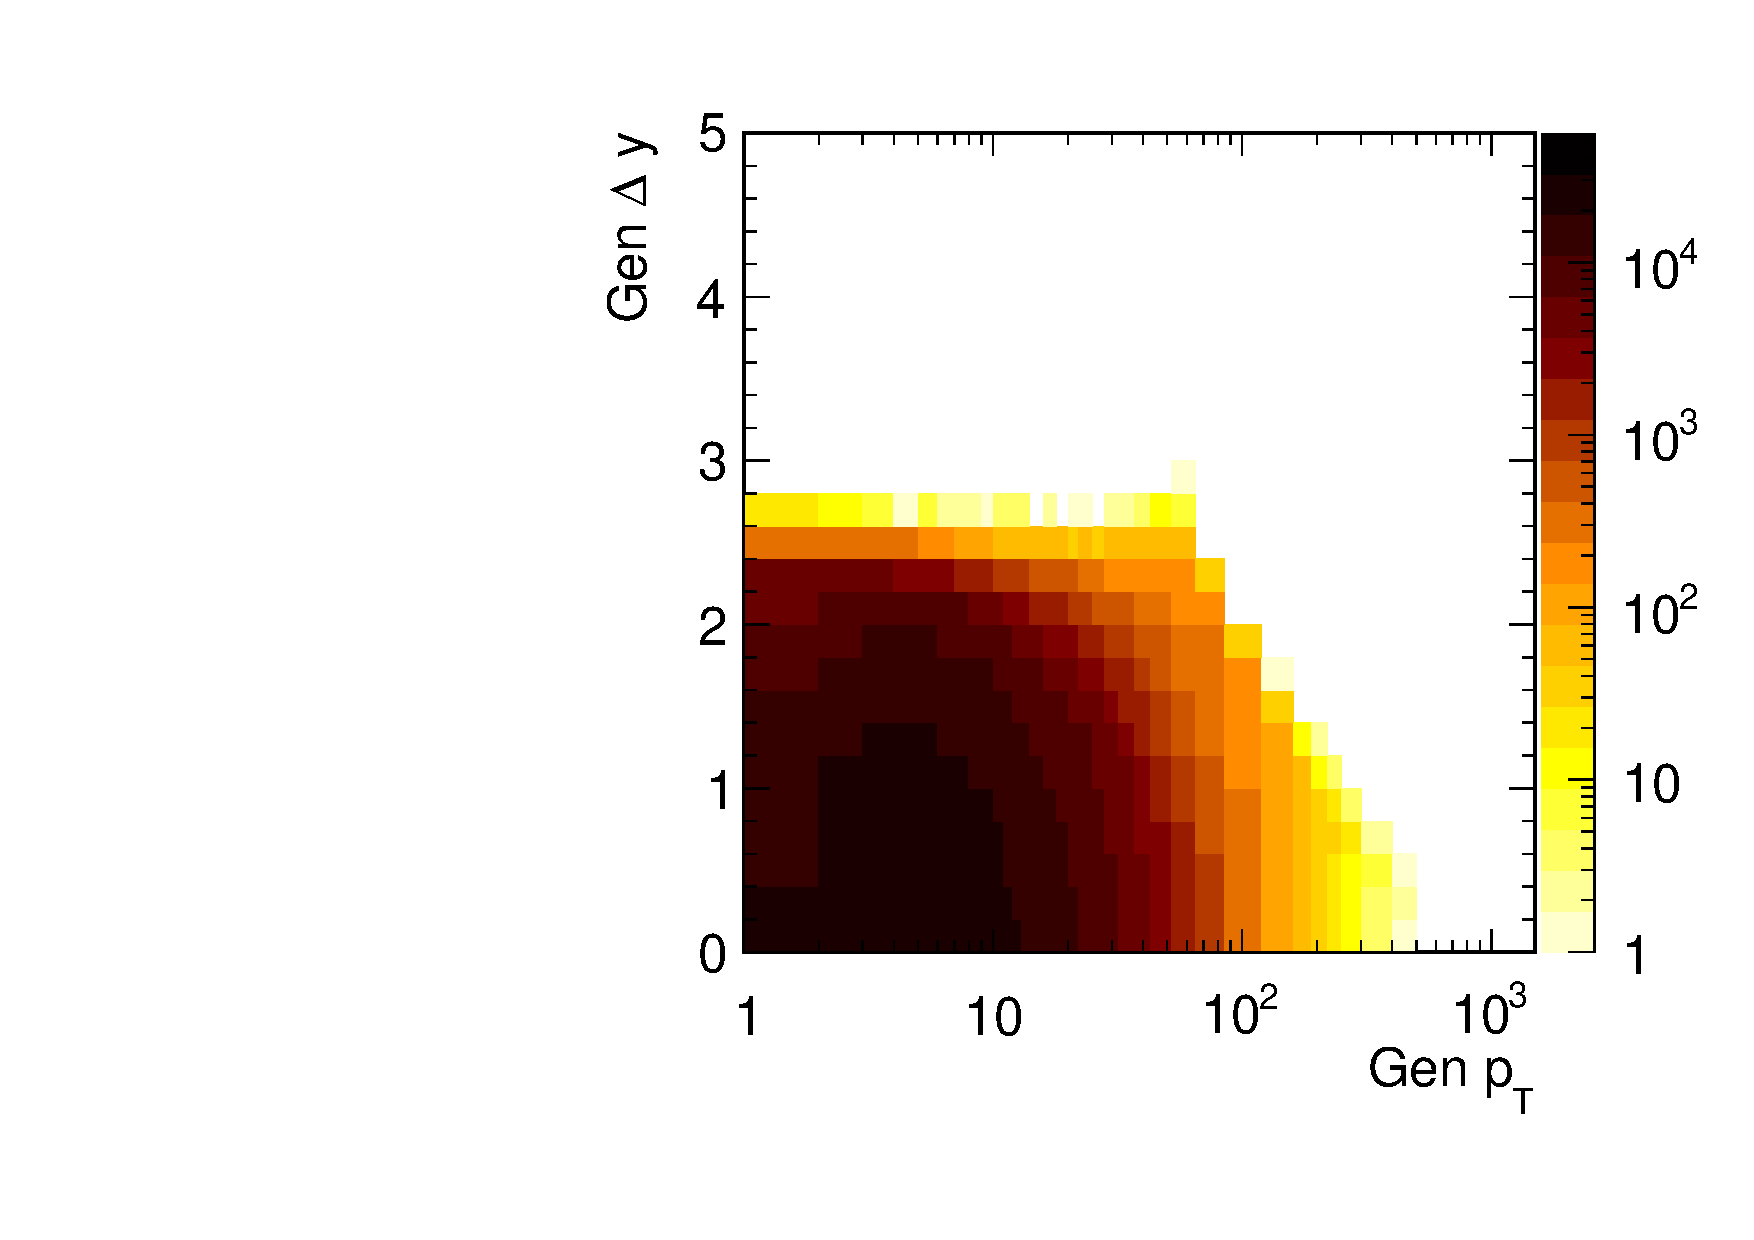
\includegraphics[width=0.49\textwidth]{figures/zpt/ptVdy.pdf}
	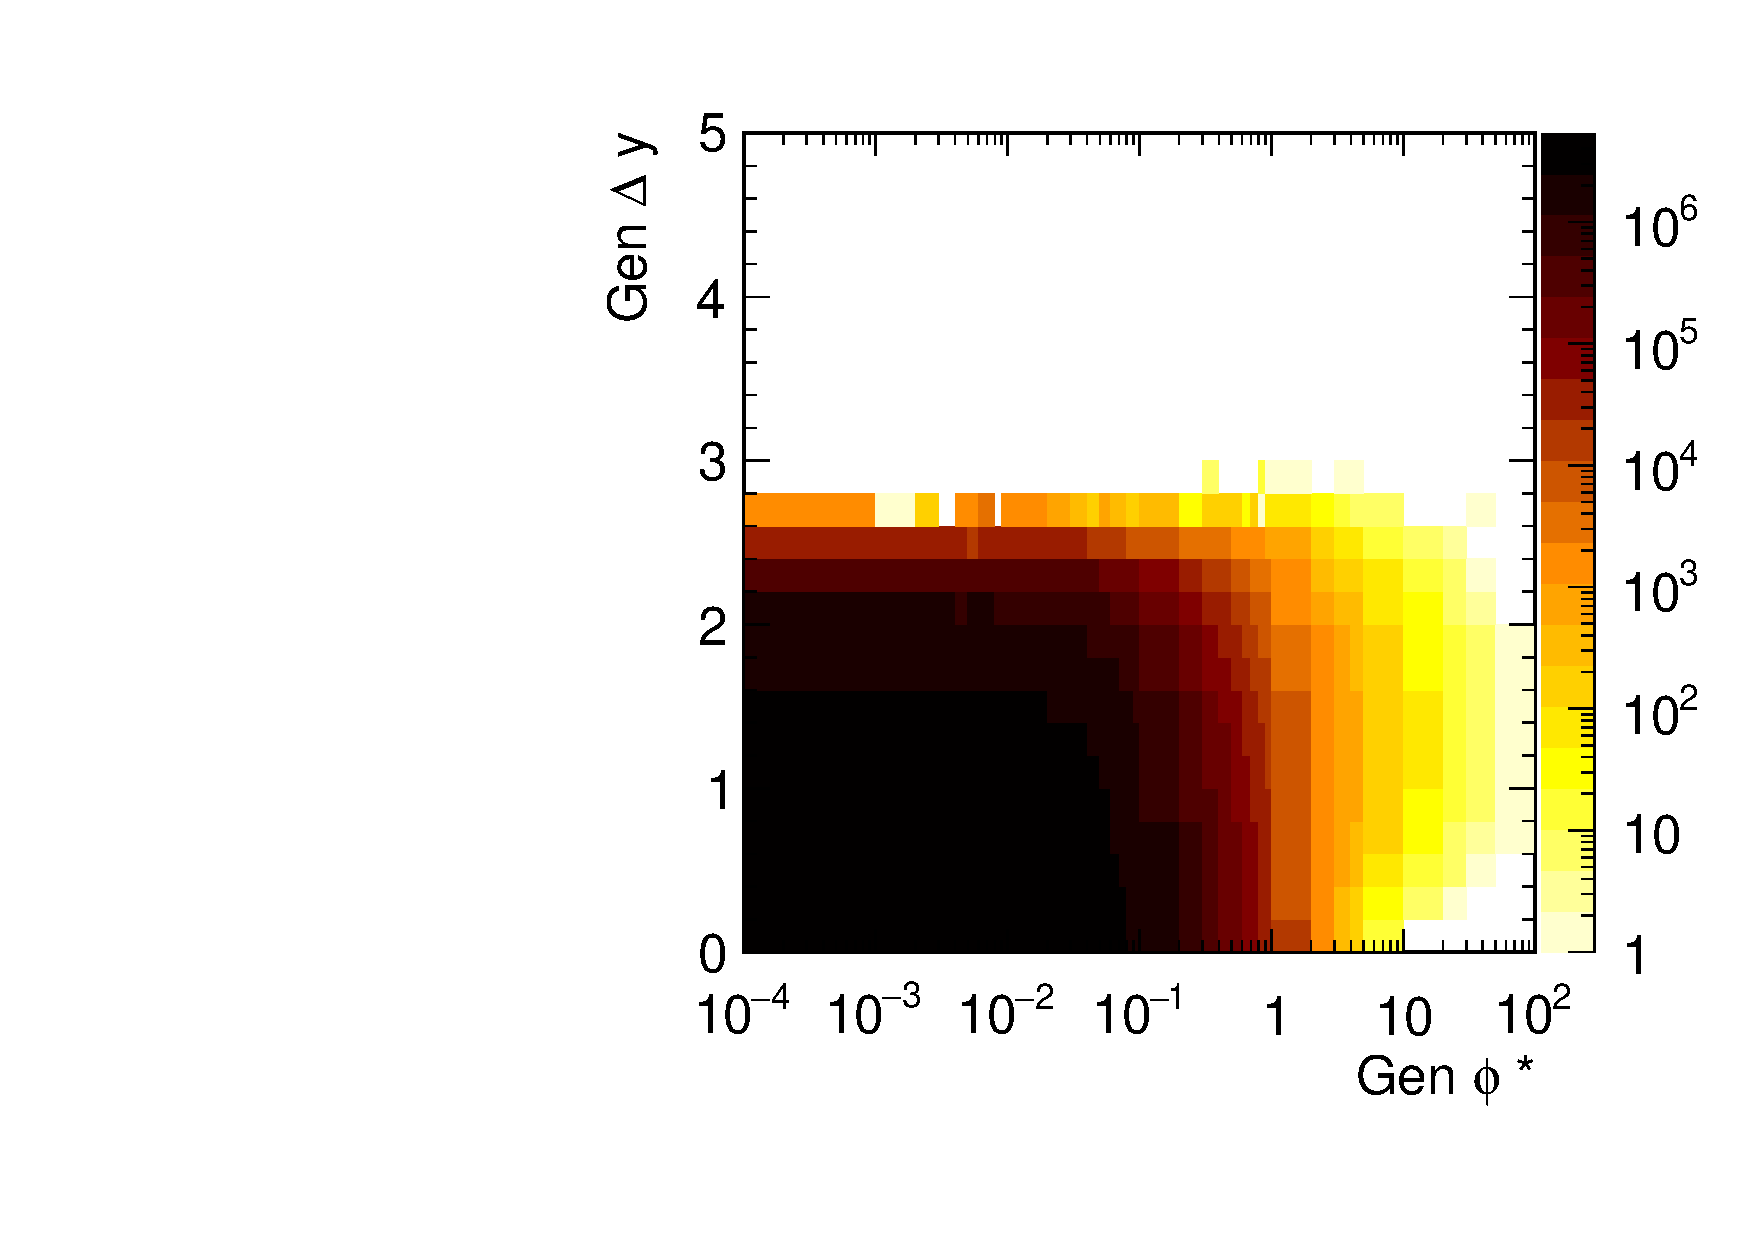
\includegraphics[width=0.49\textwidth]{figures/zpt/phiVdy.pdf}
	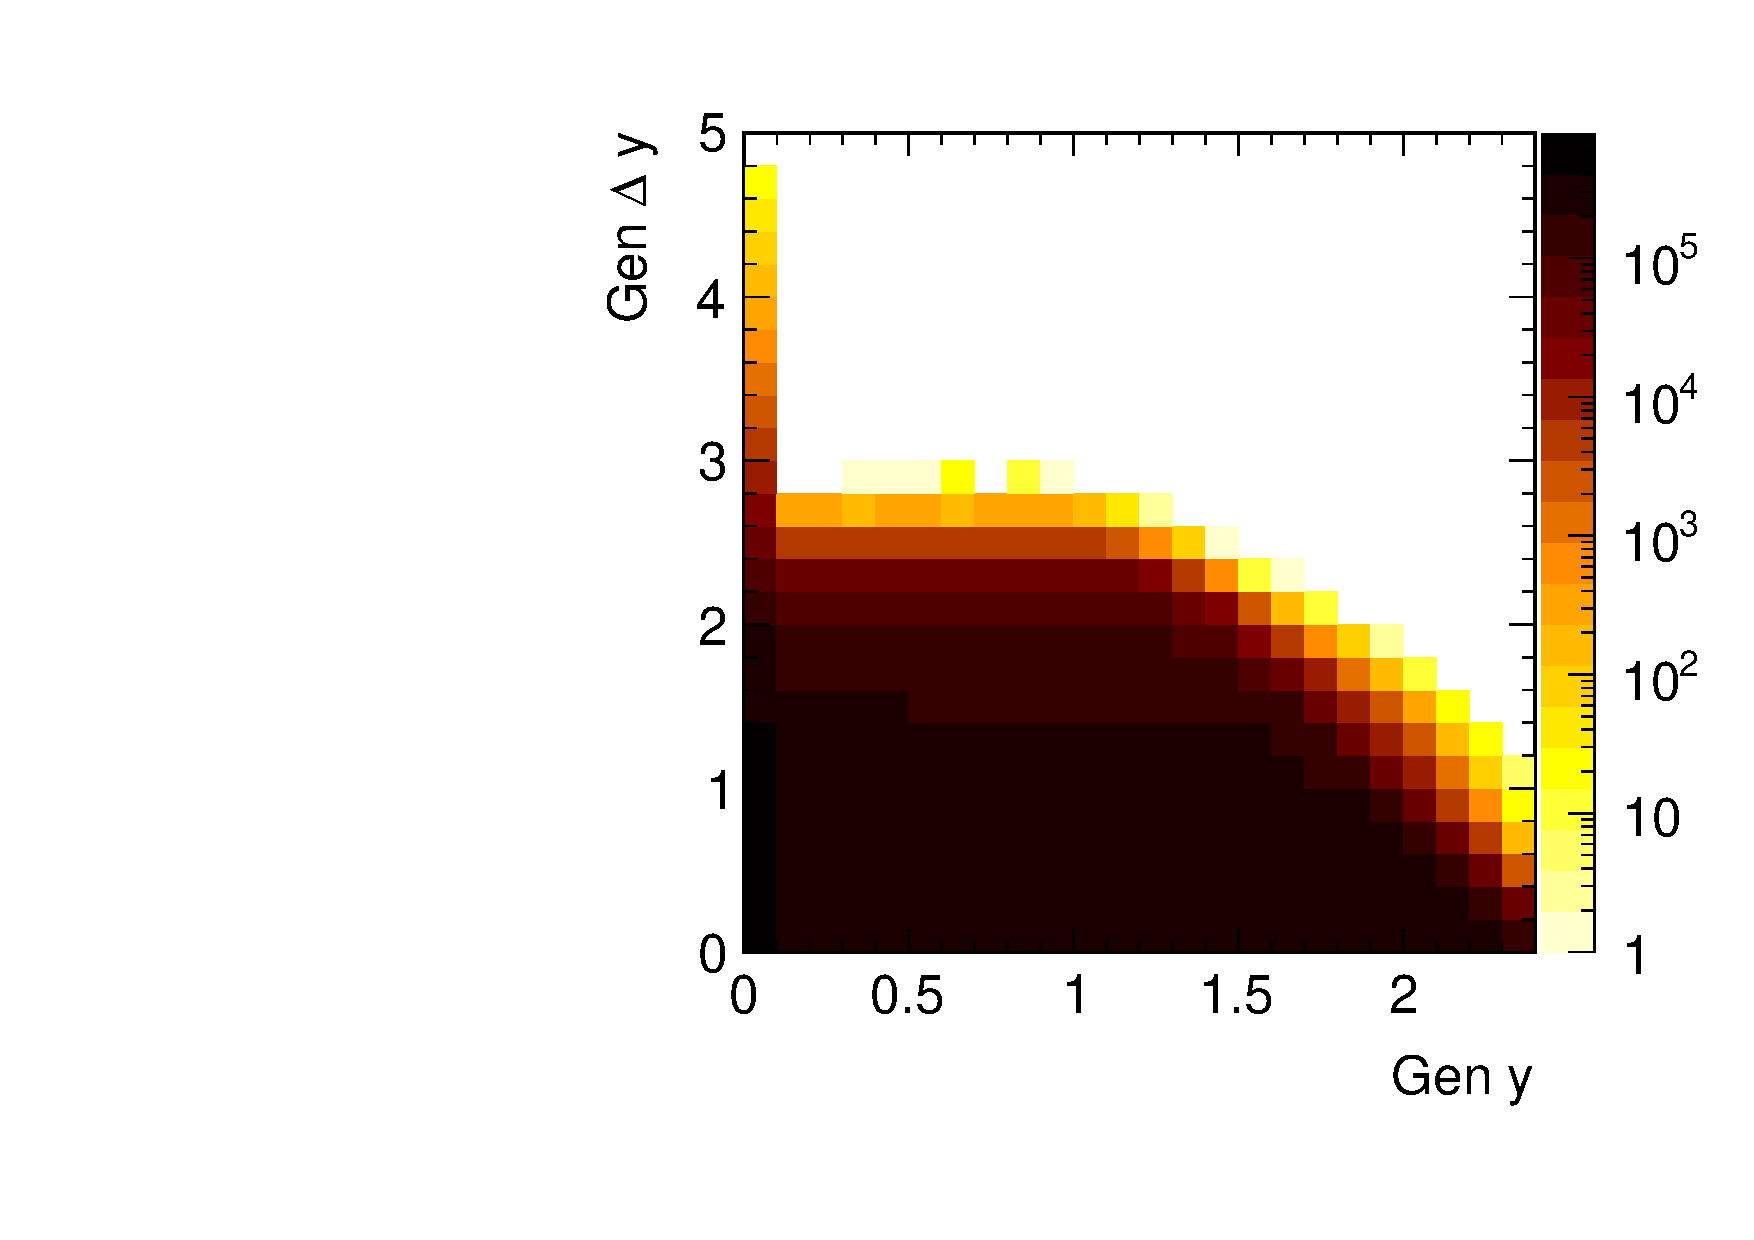
\includegraphics[width=0.49\textwidth]{figures/zpt/rapVdy.pdf}
	\caption{Distributions at the generator level of $\Delta y$ with $\pt^\Z$ (top left), $\phi^\star$ (top right), and $y^\Z$ (bottom) for dilepton pairs.}
	\label{fig:gendist3}
\end{figure}

\begin{figure}
	\centering
	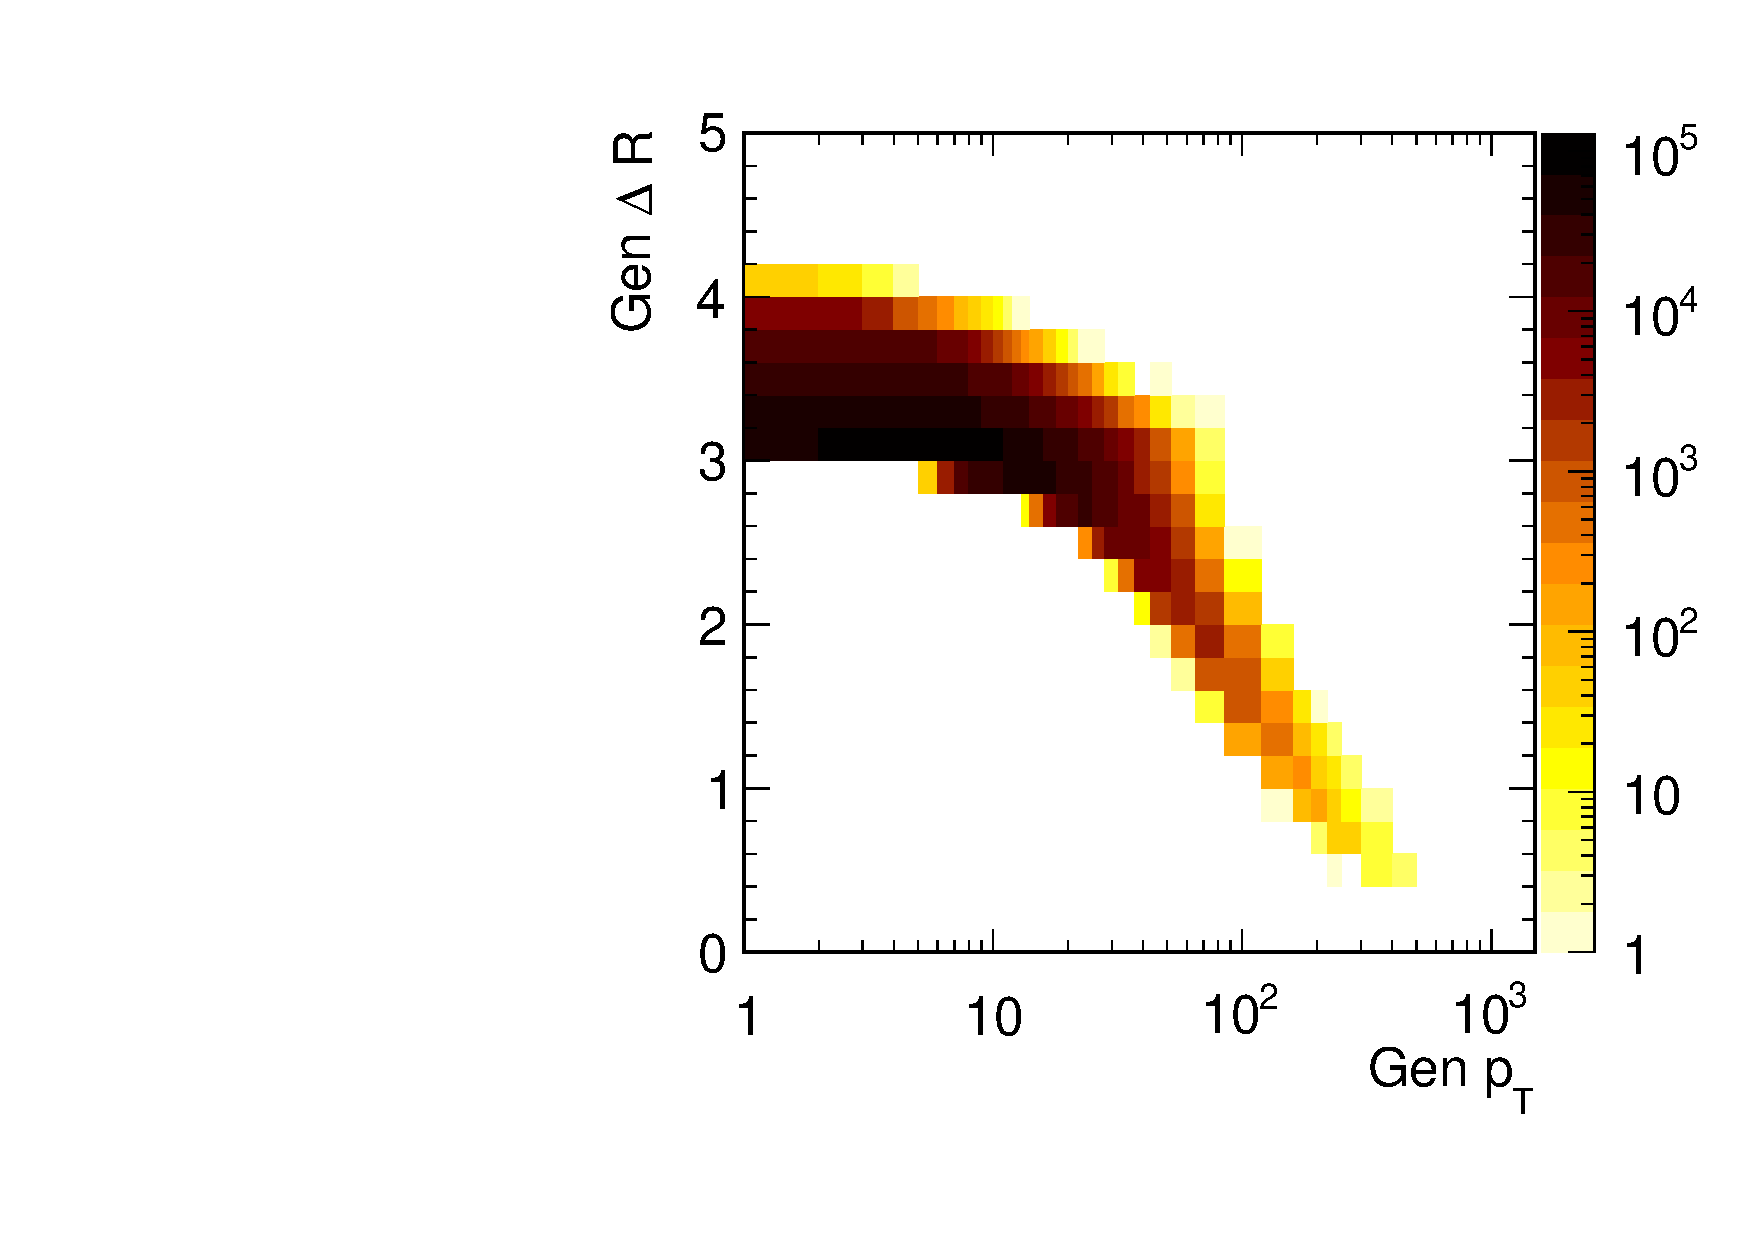
\includegraphics[width=0.49\textwidth]{figures/zpt/ptVdr.pdf}
	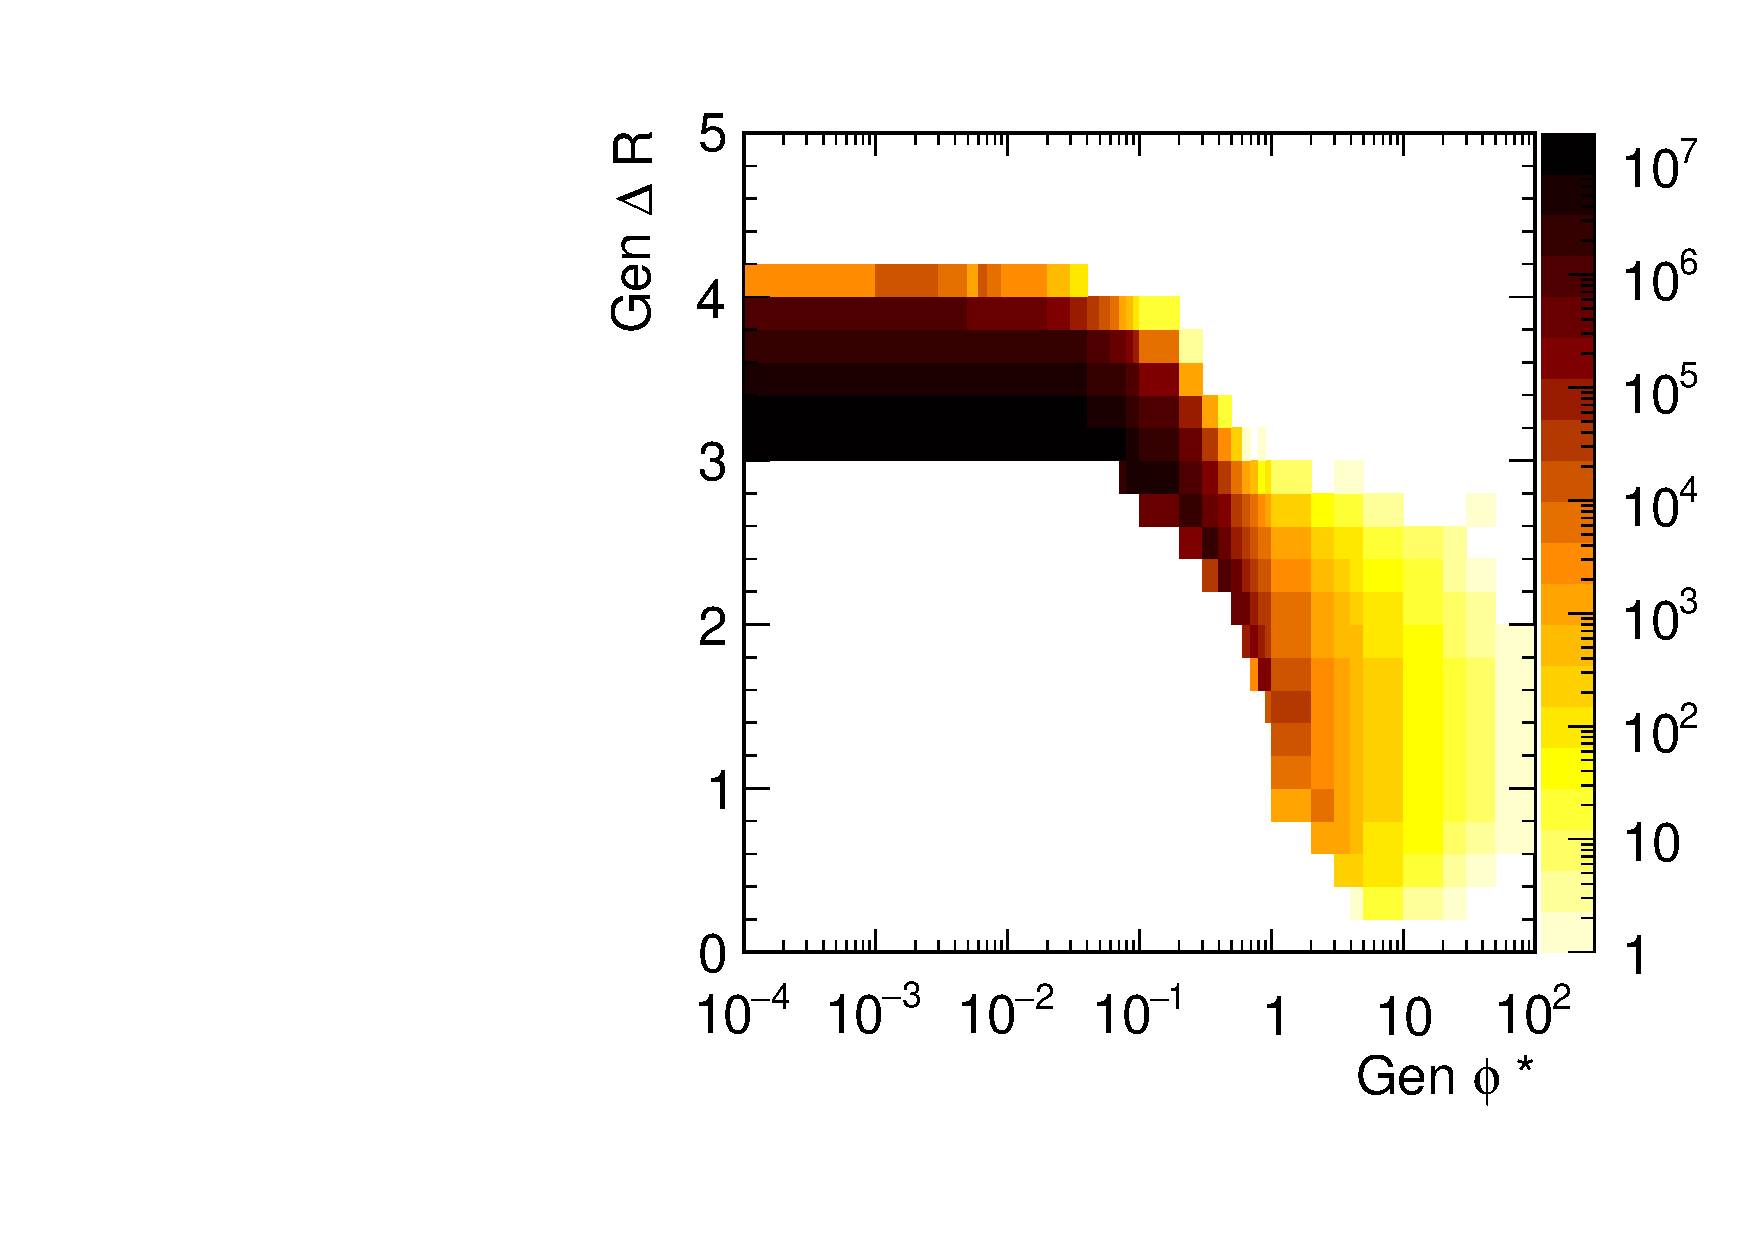
\includegraphics[width=0.49\textwidth]{figures/zpt/phiVdr.pdf}
	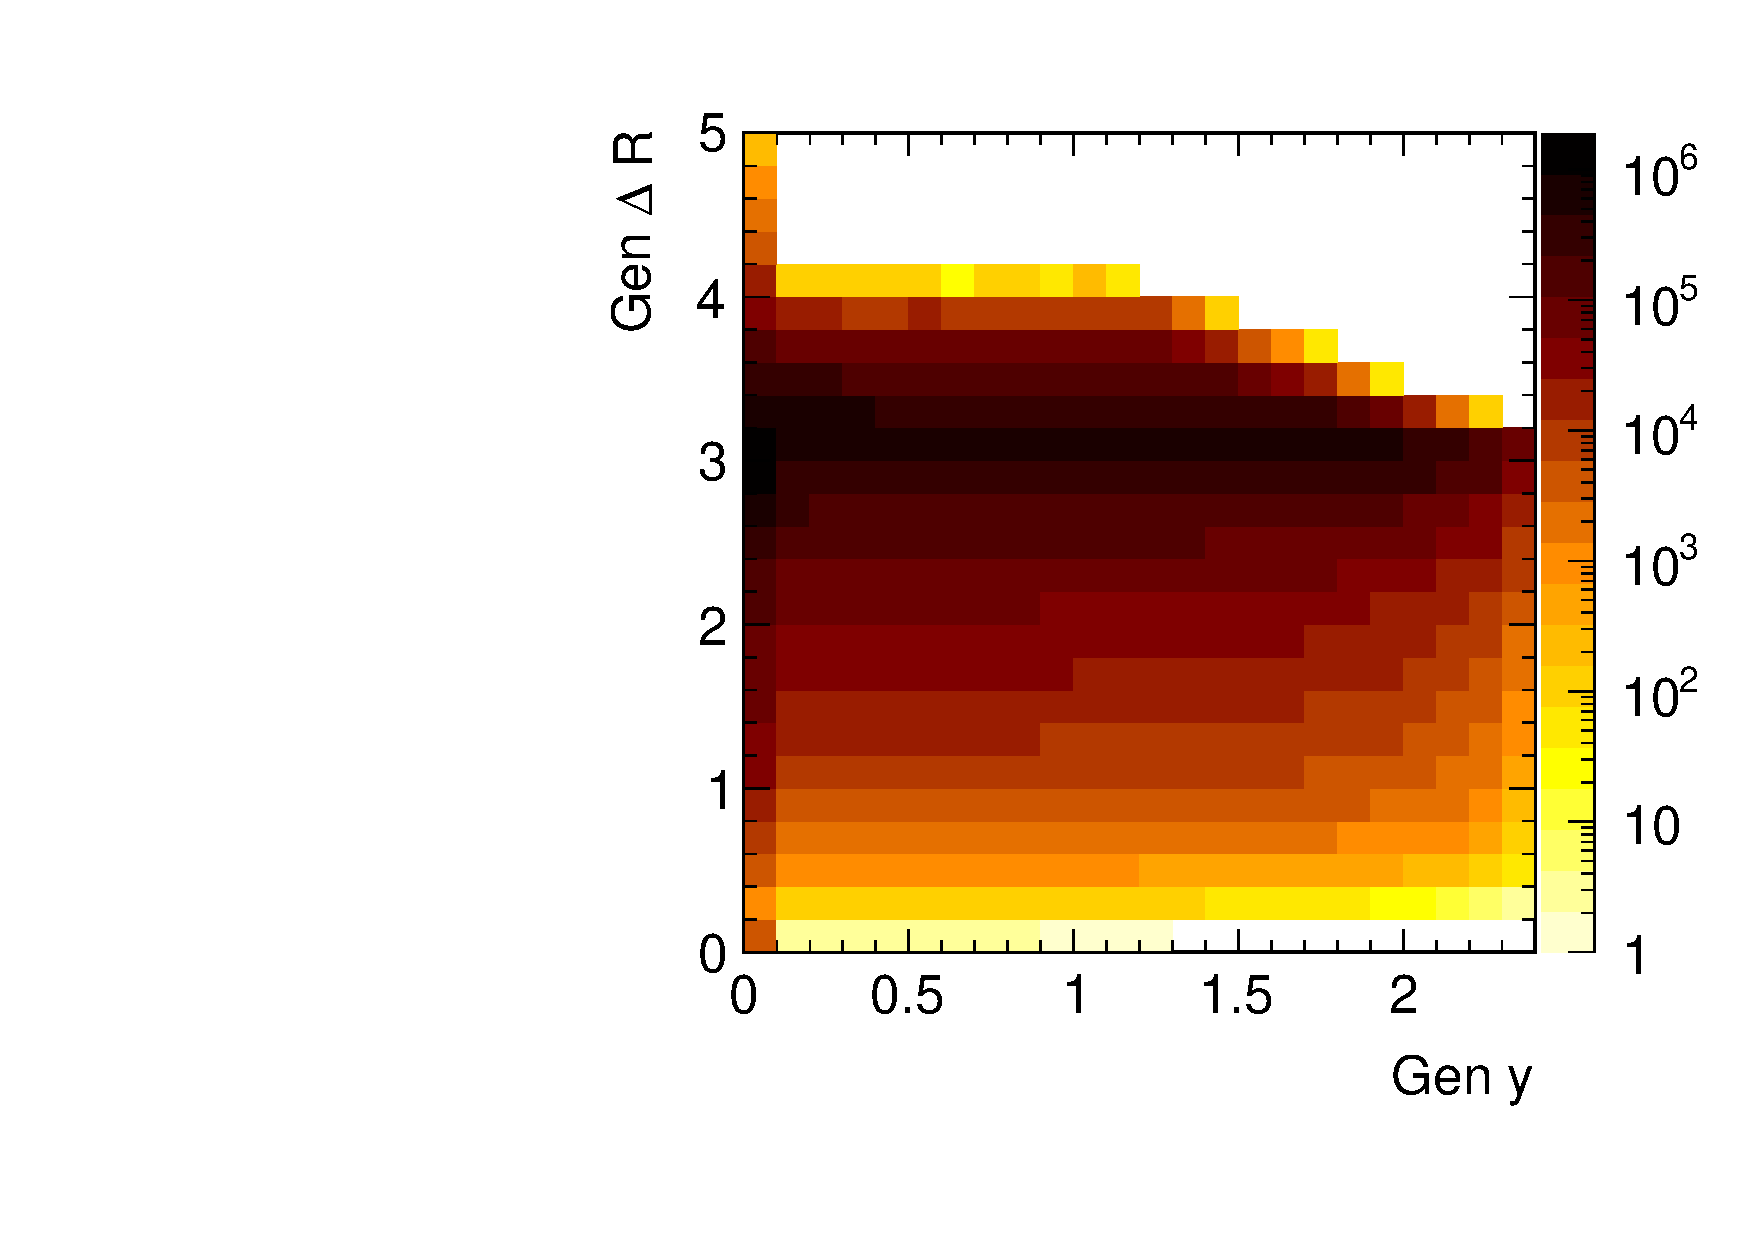
\includegraphics[width=0.49\textwidth]{figures/zpt/rapVdr.pdf}
	\caption{Distributions at the generator level of $\Delta R$ with $\pt^\Z$ (top left), $\phi^\star$ (top right), and $y^\Z$ (bottom) for dilepton pairs.}
	\label{fig:gendist4}
\end{figure}

\section{Background estimation}
\label{sec:zptbkg}
After the full selection, the amount of background processes in the data sample is 
rather small thanks to the clean signature and the relatively tight selection. 
The background processes is split into two components:
the resonant background and the nonresonant background. 
The resonant background comes from events with a real $\Z$ boson in the final state, 
e.g. $\W\Z$ diboson production; while the nonresonant background comes from events 
which do not have a $\Z$ boson in the final state.
The first set of backgrounds is estimated using a simulated events, as described in 
Section ~\ref{sec:mcsamples}. 

Nonresonant backgrounds (NRB) consist mainly 
 of leptonic $\PW$ decays in $\ttbar$, $\cPqt\PW$ decays and $\PW\PW$ events. 
 Small contributions from single top-quark events produced from
$s$-channel and $t$-channel processes, and $\cPZ\rightarrow \Pgt\Pgt$
events are also considered in this NRB estimation. 
This contribution of the nonresonant backgrounds is estimated from a control
sample of dilepton events of different flavor ($\Pe^{\pm}\Pgm^{\mp}$) 
that pass all other selection criteria.
The method has been previously used in many analyses and assumes the lepton flavor symmetry in the final states of these processes.
Since the leptonic decay branching ratios for the $ee$, $\mu\mu$ and $e\mu$ final states from NRB are 1:1:2,
the $e\mu$ events selected inside the $\Z$-mass window is extrapolated to the $ee$ and $\mu\mu$ channels.
To account for differences in efficiency for electrons and muons, 
a correction factor $k_{\mu\mu}$ is derived by comparing the NRB yields in the $ee$ and $\mu\mu$ channels:

\begin{equation}
\label{eq:kee}
k_{\mu\mu} = \frac{\epsilon_\mu}{\epsilon_{\Pe}} \approx \sqrt{\frac{N^{\mu\mu}_{NRB}}{N^{\Pe\Pe}_{NRB}}}
\end{equation}
This again assumes that each lepton leg acts independently.
The factor $k_{\mu\mu}$ is found to be about $1.3$ for the final selection, 
consistent between data and simulation. 
With this correction factor, the relation between the NRB yields in the signal and control region is:
\begin{equation}
\label{eq:nrb_xfer}
\begin{split}
  N^{\mu\mu}_{NRB}     &= \frac{1}{2} k_{\mu\mu} N^{e\mu}_{NRB} \\
  N^{\Pe\Pe}_{NRB} &= \frac{1}{2} \frac{1}{k_{\mu\mu}} N^{e\mu}_{NRB} \\
\rightarrow N^{2\ell}_{NRB}  &= \frac{1}{2} \left( k_{\mu\mu} + \frac{1}{k_{\mu\mu}} \right) N^{e\mu}_{NRB}
\end{split}
\end{equation}

A summary of the data, signal, and background yields after the full selection for the dimuon and dielectron 
final states is shown in Table~\ref{tab:zpt_yields}.

\begin{table}[hbtp]
  \begin{center}
\caption{Summary of data, signal, and background yields after the full selection. 
The signal yields are quoted using \textsc{MadGraph5\_aMC@NLO}.\label{tab:zpt_yields}}
\begin{tabular}{ccccc}
\hline
Final state      & Data & $\Z\to\ell\ell$ & Resonant bkg. & Nonresonant bkg. \\
\hline
$\mu\mu$         & $\sim 20.4 \times 10^{6}$ & $\sim 20.7 \times 10^{6}$ & $\sim 30 \times 10^{3}$ & $\sim 41 \times 10^{3}$ \\
$\Pe\Pe$         & $\sim 12.1 \times 10^{6}$ & $\sim 12.0 \times 10^{6}$ & $\sim 19 \times 10^{3}$ & $\sim 26 \times 10^{3}$ \\
\hline
  \end{tabular}
  \end{center}
\end{table}

\section{Systematic uncertainties}

In this section the systematic uncertainties taken into
account in the Z differential measurement are summarized. 
Uncertainties do not only influence the overall normalization
(\eg the uncertainty in the luminosity measurement), but also the
distribution of relevant kinematic observables (\eg the uncertainty in
the lepton momentum scale), are treated as shape uncertainties. Their
impact is evaluated by performing the full analysis 
%not only for the central value of the relevant parameter, but also
with its value shifted up and down by one standard deviation. For
each source of uncertainty, the impact in different bins of the final 
distribution is thus considered fully correlated, while
independent sources of uncertainty are treated as uncorrelated.

%%%%%%%%%%%%%%%%%%%%%%%%%%%%%%%%%%
\subsection{Sources of systematic uncertainties}
%%%%%%%%%%%%%%%%%%%%%%%%%%%%%%%%%%
The different sources of the systematic uncertainties are summarized in this section

%%%%%%%%%%%%%%%%%%%%%%%%%%%%%%%%%%
\subsubsection{Luminosity}
%%%%%%%%%%%%%%%%%%%%%%%%%%%%%%%%%%

The assigned uncertainty to the integrated luminosity measurement for
the data set used in this analysis is $\lumiunc$.

%%%%%%%%%%%%%%%%%%%%%%%%%%%%%%%%%%
\subsubsection{Trigger, lepton reconstruction and identification efficiencies}
%%%%%%%%%%%%%%%%%%%%%%%%%%%%%%%%%%

Discrepancies in the lepton reconstruction and identification
efficiencies between data and simulation are corrected by applying
to all MC samples 
data-to-simulation scale factors measured using $\dyll$ events in the $\cPZ$
peak region~\cite{wzxs} that are recorded with unbiased triggers. These factors
depend on the lepton $\pt$ and $\eta$ and are within 2\% for electrons and muons.
The uncertainty in the determination of the trigger efficiency leads to an uncertainty 
smaller than 1\% in the expected signal yield. Residual difference between the analysis 
lepton requirements with respect to the trigger selections is well covered by 
the uncertainty in the trigger efficiency. The uncertainty due to 
the muon (electron) reconstruction efficiency varies between 0.1\% (0.2\%) in the central 
part of the detector up to (0.4\%) (1.0\%) at large $|\eta|$ values. 
The uncertainty due to the lepton identification selection is about 0.4\% per muon leg, and 
about 1.1\% per electron leg, although with a sizable dependence on $\eta$ and $\pt$.
The precise methodology of determining these identification scale factors has been expounded above,
in Chapter~\ref{chap:efficiency}.
The trigger and reconstruction efficiencies are measured in similar ways,
but the fitting procedure is comparatively trivial due to high purity.

%%%%%%%%%%%%%%%%%%%%%%%%%%%%%%%%%%
\subsubsection{Lepton momentum scale and resolution}
%%%%%%%%%%%%%%%%%%%%%%%%%%%%%%%%%%

The lepton momentum scale uncertainty is computed by varying the
momentum of the leptons by their uncertainties. The effect 
on the analysis is rather small, except for very low or very high dilepton 
$\pt$.

%%%%%%%%%%%%%%%%%%%%%%%%%%%%%%%%%%
\subsubsection{L1 pre-firing trigger inefficiency}
%%%%%%%%%%%%%%%%%%%%%%%%%%%%%%%%%%
The L1 pre-firing trigger inefficiency is an experimental issue in the data recorded in 2016
which reduces the number of selected events.
In addition, it introduces  a sizable uncertainty
since it is not easy to precisely measure this effect.

The root of the problem is the ECAL trigger primitive (TP) timing.
When an ECAL TP pre-fires, its entire energy is assigned to the bunch crossing numbered -1 (BX-1).
The trigger rules dictate that after a L1 trigger firing, the next 2 bunch crossings are not available for firing.
Thus, if the energy of the TP is large enough to pre-fire a L1 trigger in BX-1,
any physics event in BX0 or BX1 is lost. 
In contrast, if the BX-1 is not accepted,
a residual effect on BX0 is present because a null energy is associated with the 
early TP. Finally, the TP inputs are used by the ECAL selective readout units 
(SRPs) to decide whether a certain region of the detector needs to be fully 
readout or zero-suppressed. Crystals associated with the early TP will be readout 
in zero-suppression mode, injecting a bias in the HLT/offline energy measurement.

The effect can be measured in data by selecting un-prefirable events at BX0, where the L1 trigger fired in BX-3.
In that case, by the trigger rules BX-2 and BX-1 cannot possibly have fired the L1 trigger, so BX0 is a clean slate.
Unfortunately, the rate of un-prefirable events 
is rather small compared to the total data sample, about $0.1\%$, and therefore 
the statistical precision of that effect is a concern. 

Overall, the recommended uncertainty is about 20\% of the correction. This translates 
to a rather small impact on the inclusive analysis, but it leads to a sizable impact 
on the $\Z$ boson rapidity measurement.

Because this effect directly affects the lepton and event reconstruction, the
corresponding uncertainty has been merged together with the standard lepton
reconstruction efficiency uncertainties.

%%%%%%%%%%%%%%%%%%%%%%%%%%%%%%%%%%
\subsubsection{Background subtraction}
%%%%%%%%%%%%%%%%%%%%%%%%%%%%%%%%%%

The resonant background processes are estimated from simulation, so
the uncertainties on 
the normalization are derived from variations of the QCD scale, $\alpha_{s}$ and 
parton distribution functions (PDFs) variations~\cite{Botje:2011sn,Alekhin:2011sk,Lai:2010vv,Martin:2009iq,Ball:2011mu,MCFM}. 
The PDF and $\alpha_s$ uncertainties for signal and background processes are estimated 
from the standard deviation of weights from the replicas provided in the 
NNPDF3.0 parton distribution set~\cite{nnpdf}.

The procedure for estimating uncertainties arising from Parton
Distribution Functions (PDF uncertainties) follows the recommendations
issued by the PDF4LHC group \cite{Butterworth:2015oua}.
For the second run of the LHC, the PDF4LHC group has provides a set of combined
PDF sets -- the PDF4LHC pdf sets -- which are used in the following for the estimation
of PDF uncertainty.

The uncertainty in the nonresonant background is estimated to the be 
about 5\%, which is rather conservative, but it makes barely any difference in
this analysis.

%%%%%%%%%%%%%%%%%%%%%%%%%%%%%%%%%%
\subsubsection{Model dependence in unfolding}
%%%%%%%%%%%%%%%%%%%%%%%%%%%%%%%%%%

Model dependence of unfolding is due to the folding of the detector resolution 
with the expected spectra. Unfolding is expected to work properly if these 
differences are small and the predicted migration relative contribution between 
the bins close to the correct value. In order to keep this effect under control 
a different matrix can be constructed starting from a different \MC{} generator; 
this generator should be full reconstructed in order to correctly account for 
the bin-migrations. Alternatively, one could try to reweight the \MC{} to 
match other predicted spectra. 
Model dependence is evaluated unfolding the data with the different models and 
symmetrizing the uncertainties.

%%%%%%%%%%%%%%%%%%%%%%%%%%%%%%%%%%
\subsubsection{Statistical uncertainty estimation}
%%%%%%%%%%%%%%%%%%%%%%%%%%%%%%%%%%

The computation of the statistical uncertainty estimation after unfolding is 
complicated by the bias introduced by the unfolding itself. A ``proper'' way 
of doing this step is not fully established from the statistical point of view, 
making this an active field of research \cite{Prosper:2011zz,kuusela}.
Different toys and resampling techniques are available in order to perform such 
operation, that usually provide a better coverage with respect to the analytical 
error propagation. The toy generation is performed by \RooUnfold{} smearing the 
data distribution using Gaussian uncertainties corresponding to the histogram 
errors.

%%%%%%%%%%%%%%%%%%%%%%%%%%%%%%%%%%
\subsection{Correlations} 
%%%%%%%%%%%%%%%%%%%%%%%%%%%%%%%%%%
The correlations among the different bins and the two final states used in the 
analysis are described in this section.

All the systematic uncertainties are considered to be correlated among the 
different bins for a single variable, with the exception of the uncertainties with statistical nature. 
The statistical uncertainties of the MC{} samples are treated 
as uncorrelated quantities among the different bins. In addition, the statistical 
uncertainties in the lepton efficiency scale factors for each lepton $\eta$ and $\pt$ 
bin used for such measurements are treated as uncorrelated quantities. 

When combining the muon and electron channels, the luminosity, background estimation, 
and modelling uncertainties are treated as correlated parameters, all others are 
considered as uncorrelated between them.

%%%%%%%%%%%%%%%%%%%%%%%%%%%%%%%%%%
\subsection{Total systematic uncertainty} 
%%%%%%%%%%%%%%%%%%%%%%%%%%%%%%%%%%

A graphical representation of the different contributions to the systematic uncertainty 
is shown in Figures~\ref{fig:zpt_syst0},~\ref{fig:zpt_syst1}, and~\ref{fig:zpt_syst2}. 
A summary of the systematic uncertainties related to the lepton efficiency measurements 
of muons and electrons is shown in Figure~\ref{fig:zpt_systeff}.

\begin{figure}
	\centering
	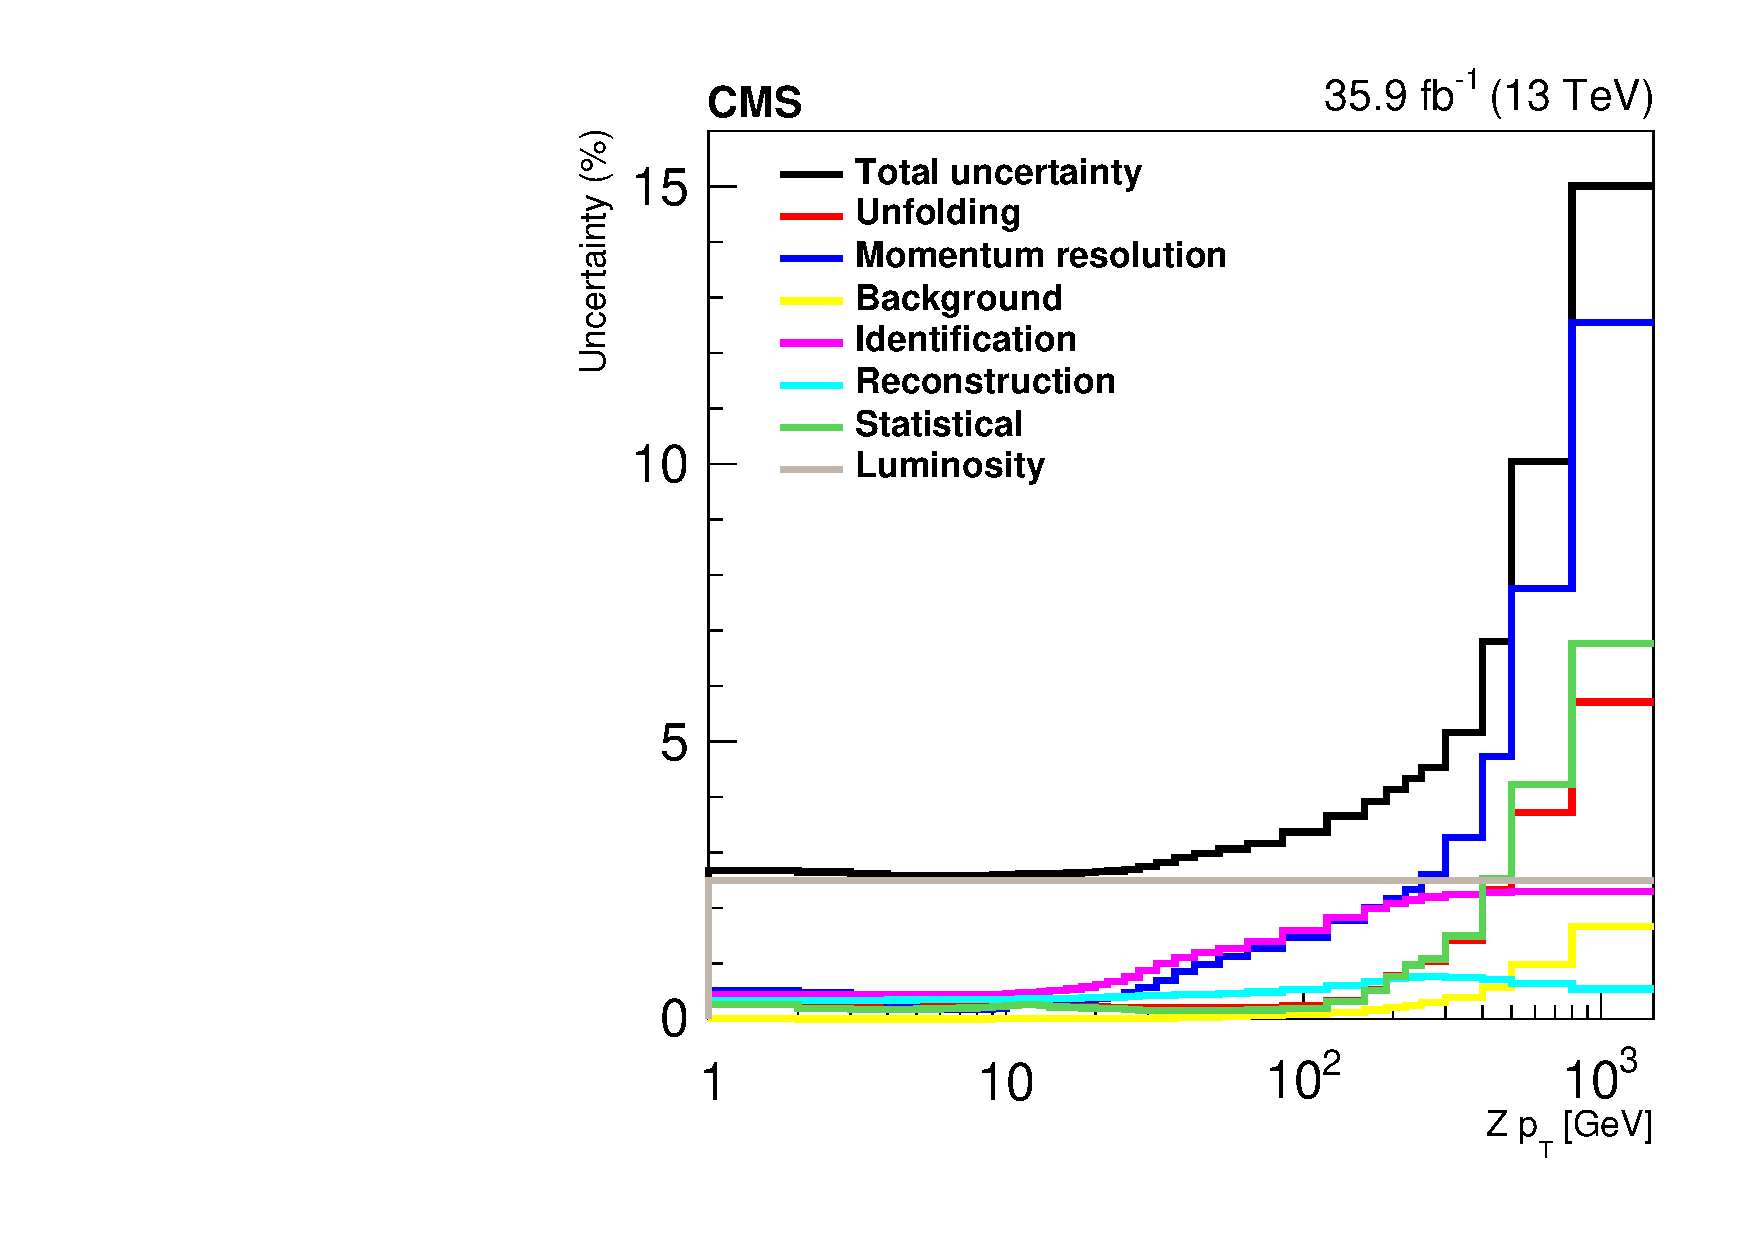
\includegraphics[width=0.49\textwidth]{figures/zpt/histoUnfoldingSystPt_nsel0_dy3.pdf}
        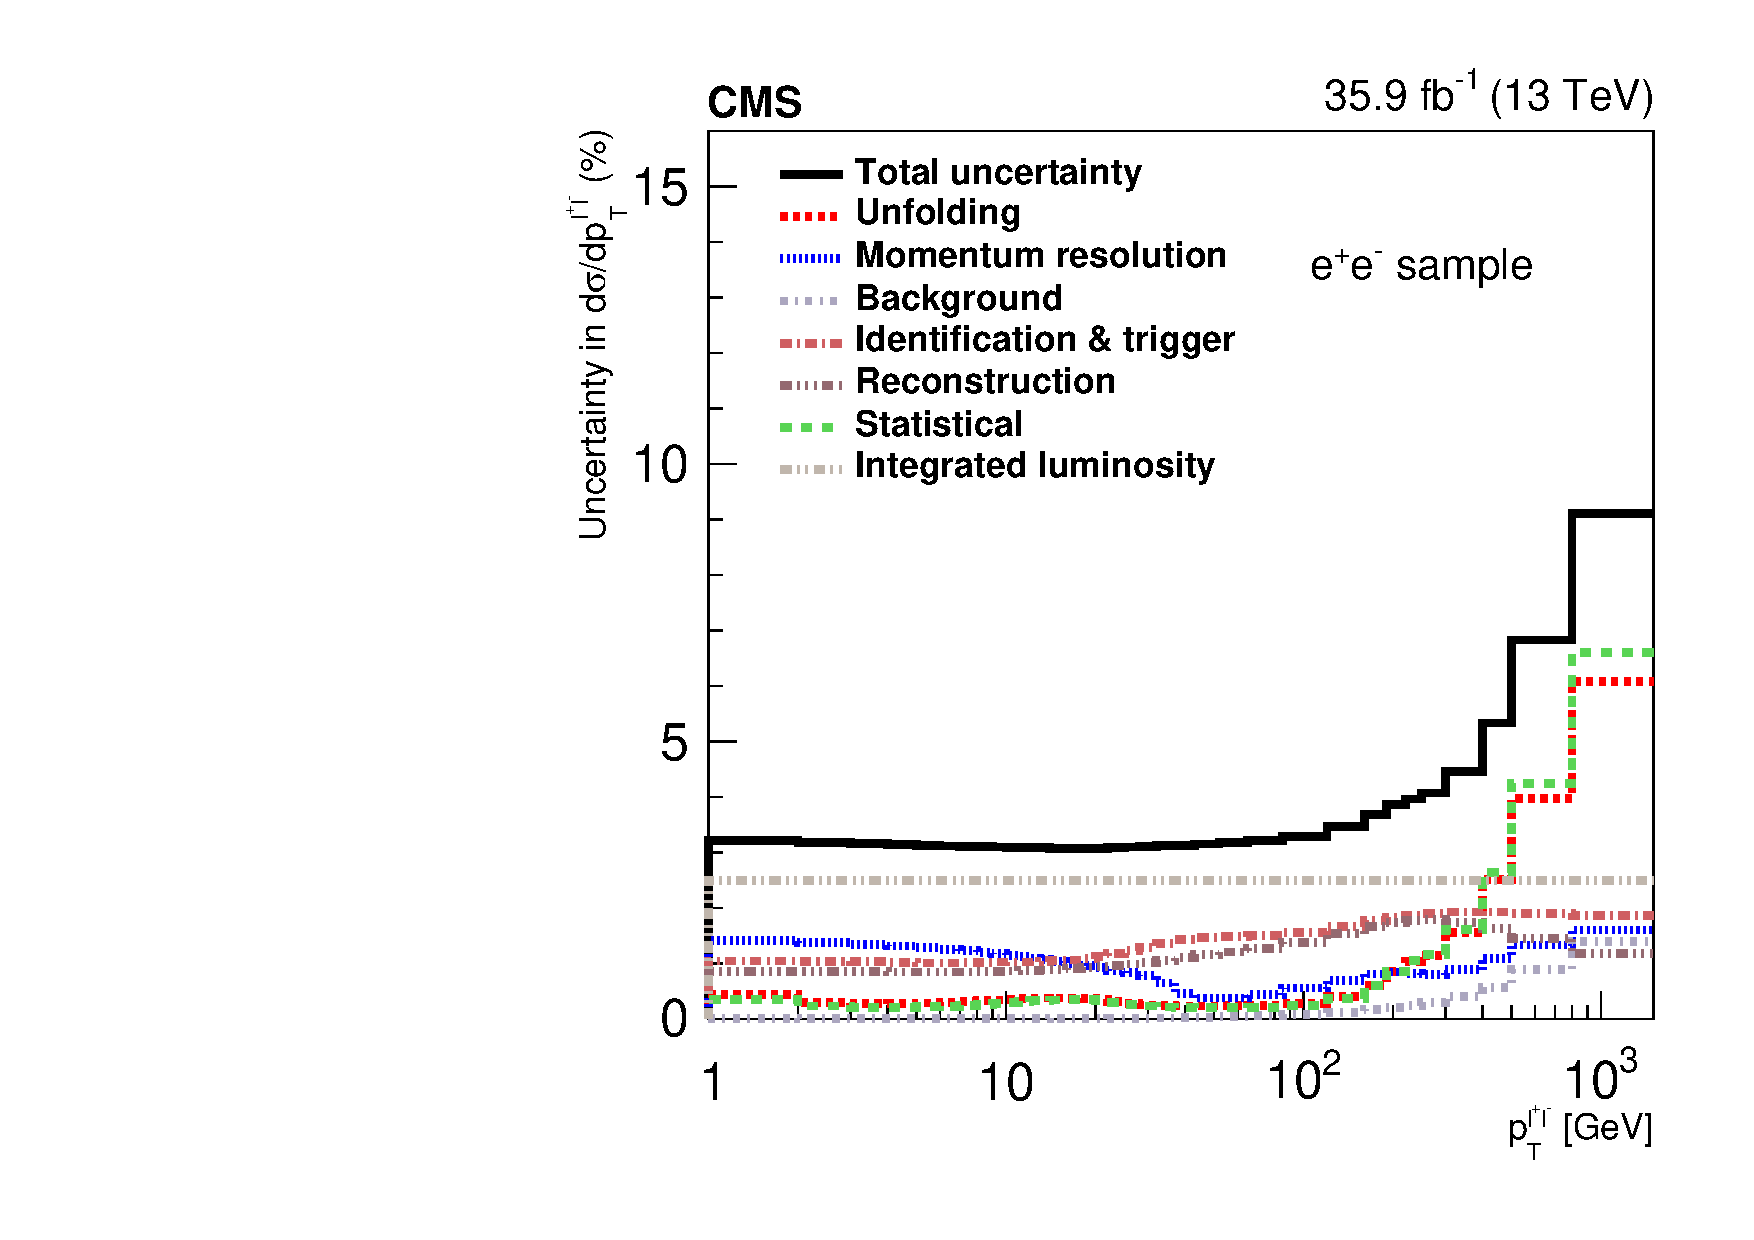
\includegraphics[width=0.49\textwidth]{figures/zpt/histoUnfoldingSystPt_nsel1_dy3.pdf}
	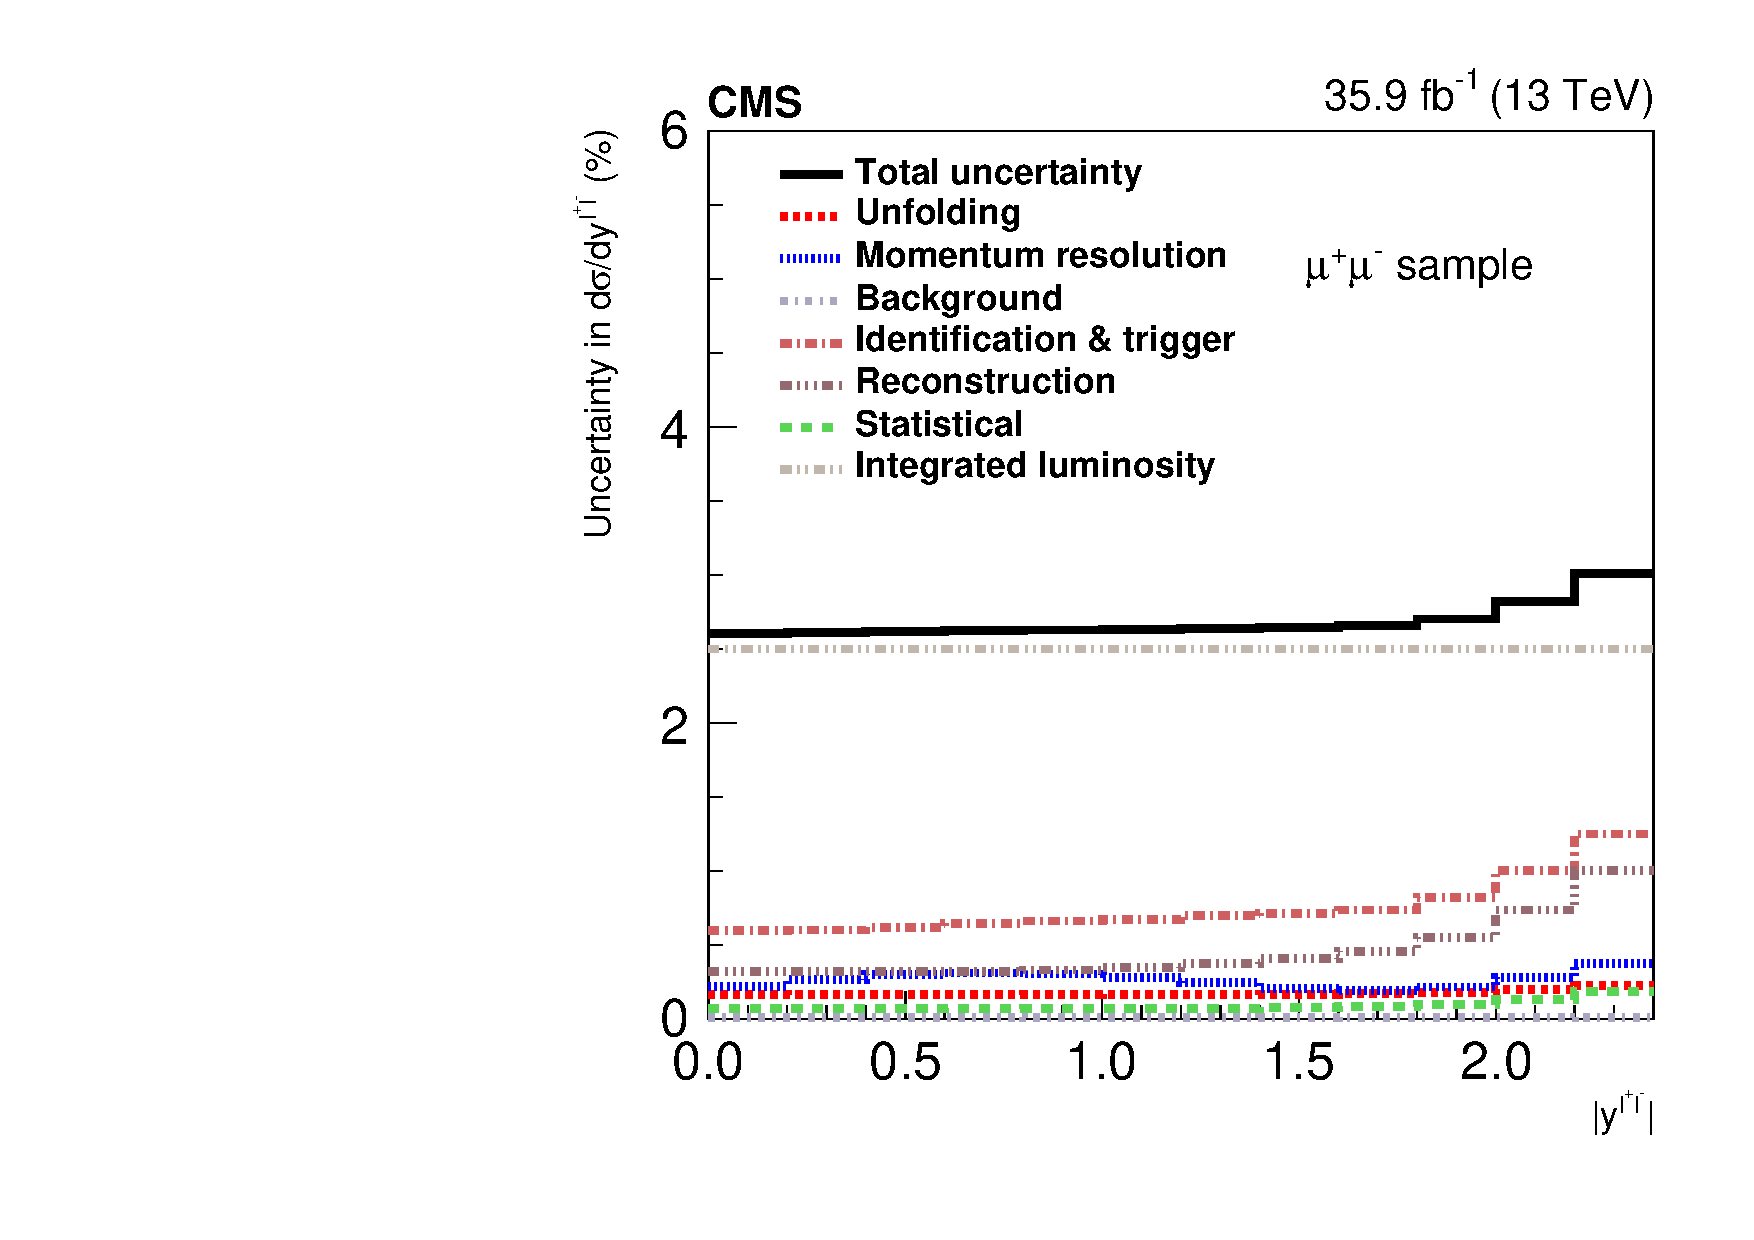
\includegraphics[width=0.49\textwidth]{figures/zpt/histoUnfoldingSystRap_nsel0_dy3.pdf}
        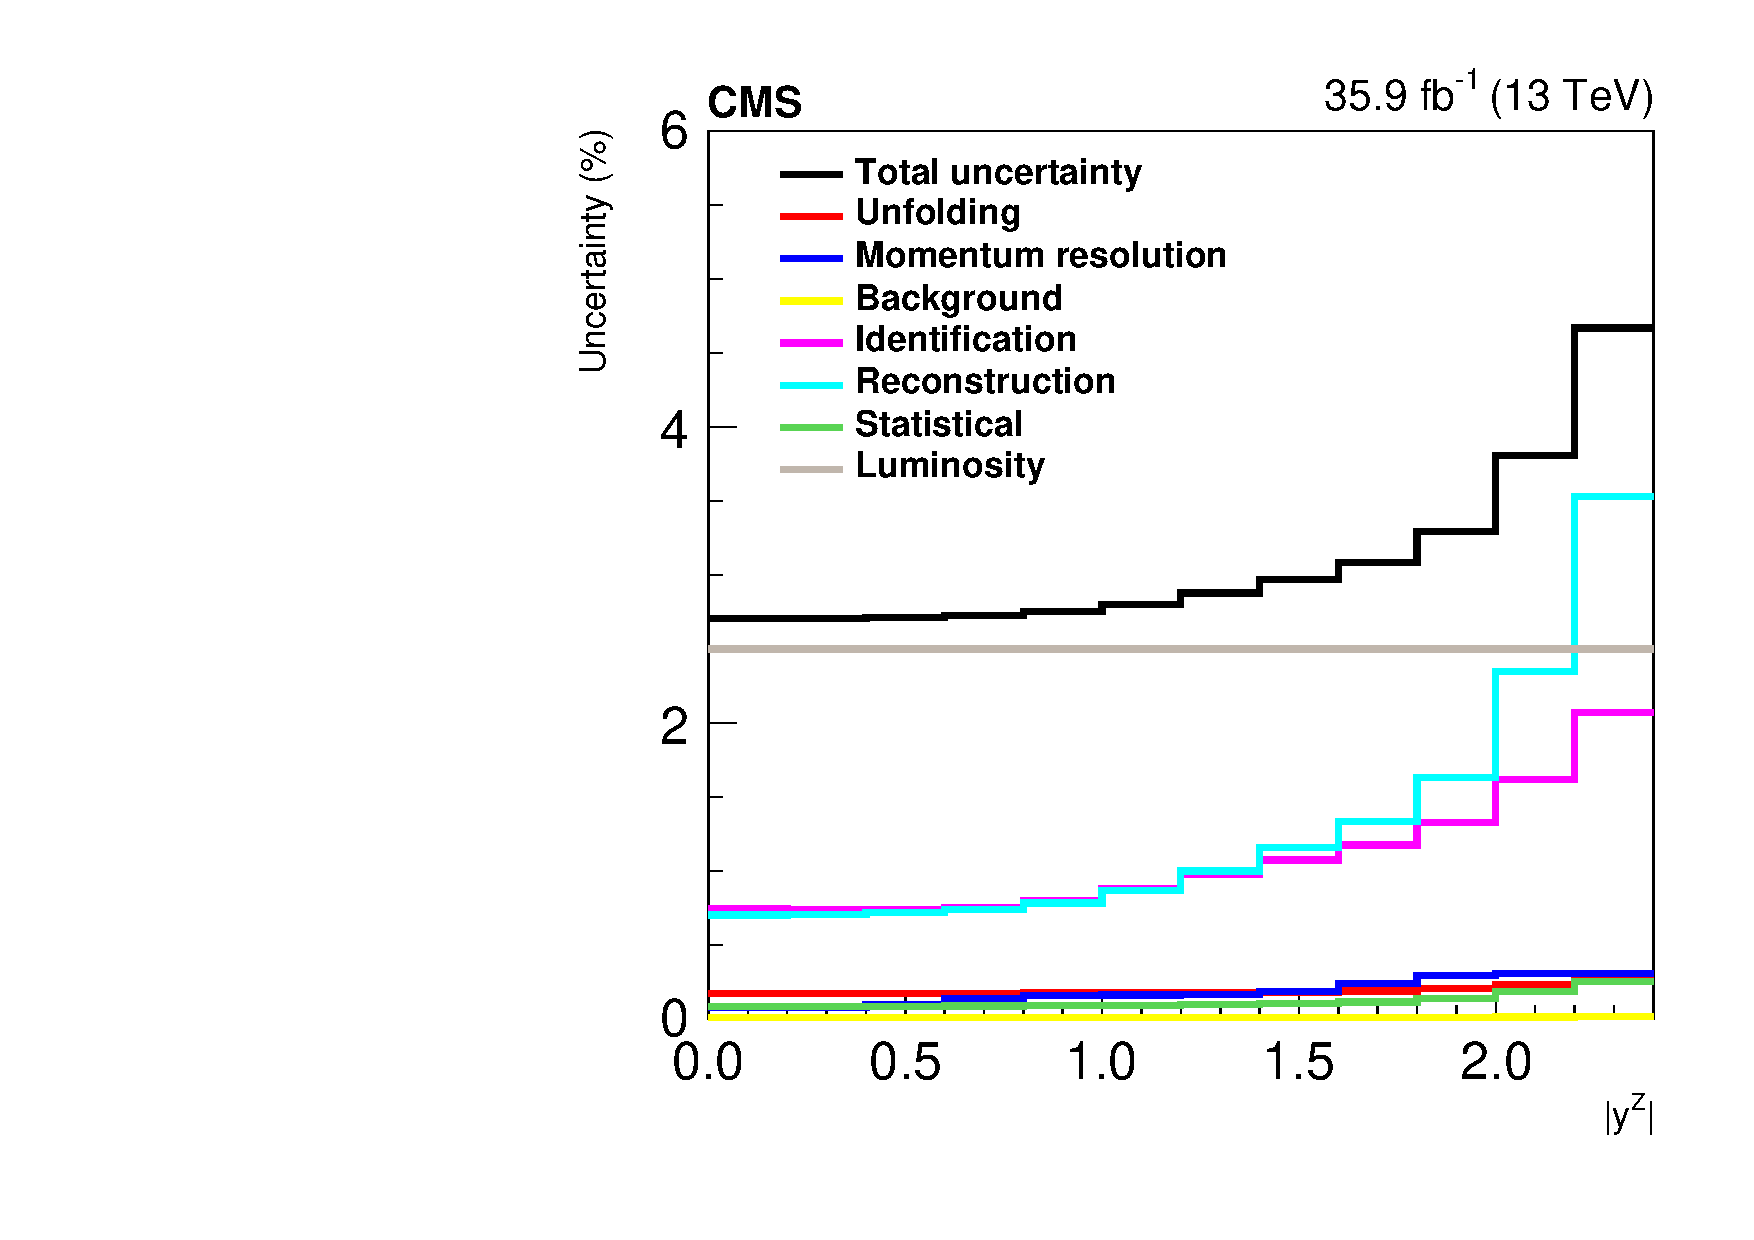
\includegraphics[width=0.49\textwidth]{figures/zpt/histoUnfoldingSystRap_nsel1_dy3.pdf}
	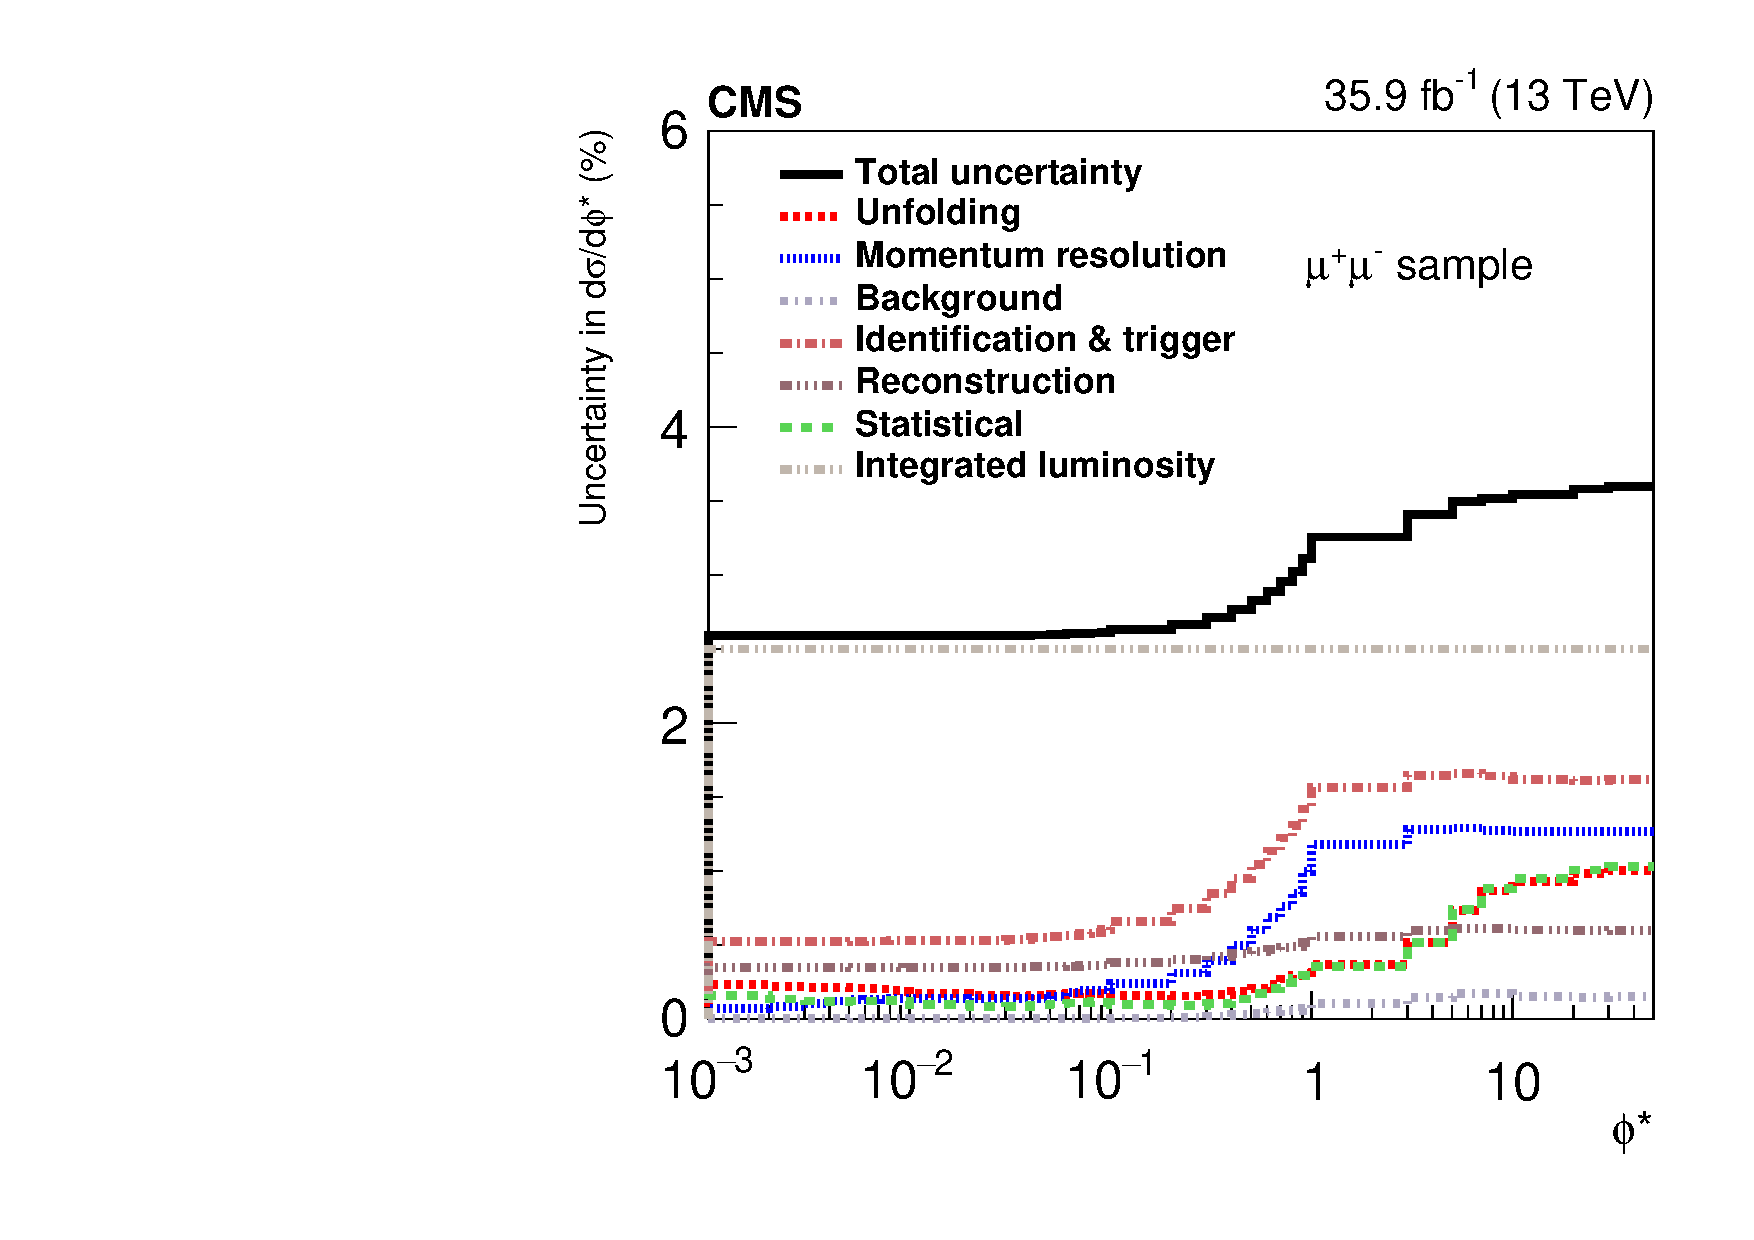
\includegraphics[width=0.49\textwidth]{figures/zpt/histoUnfoldingSystPhiStar_nsel0_dy3.pdf}
        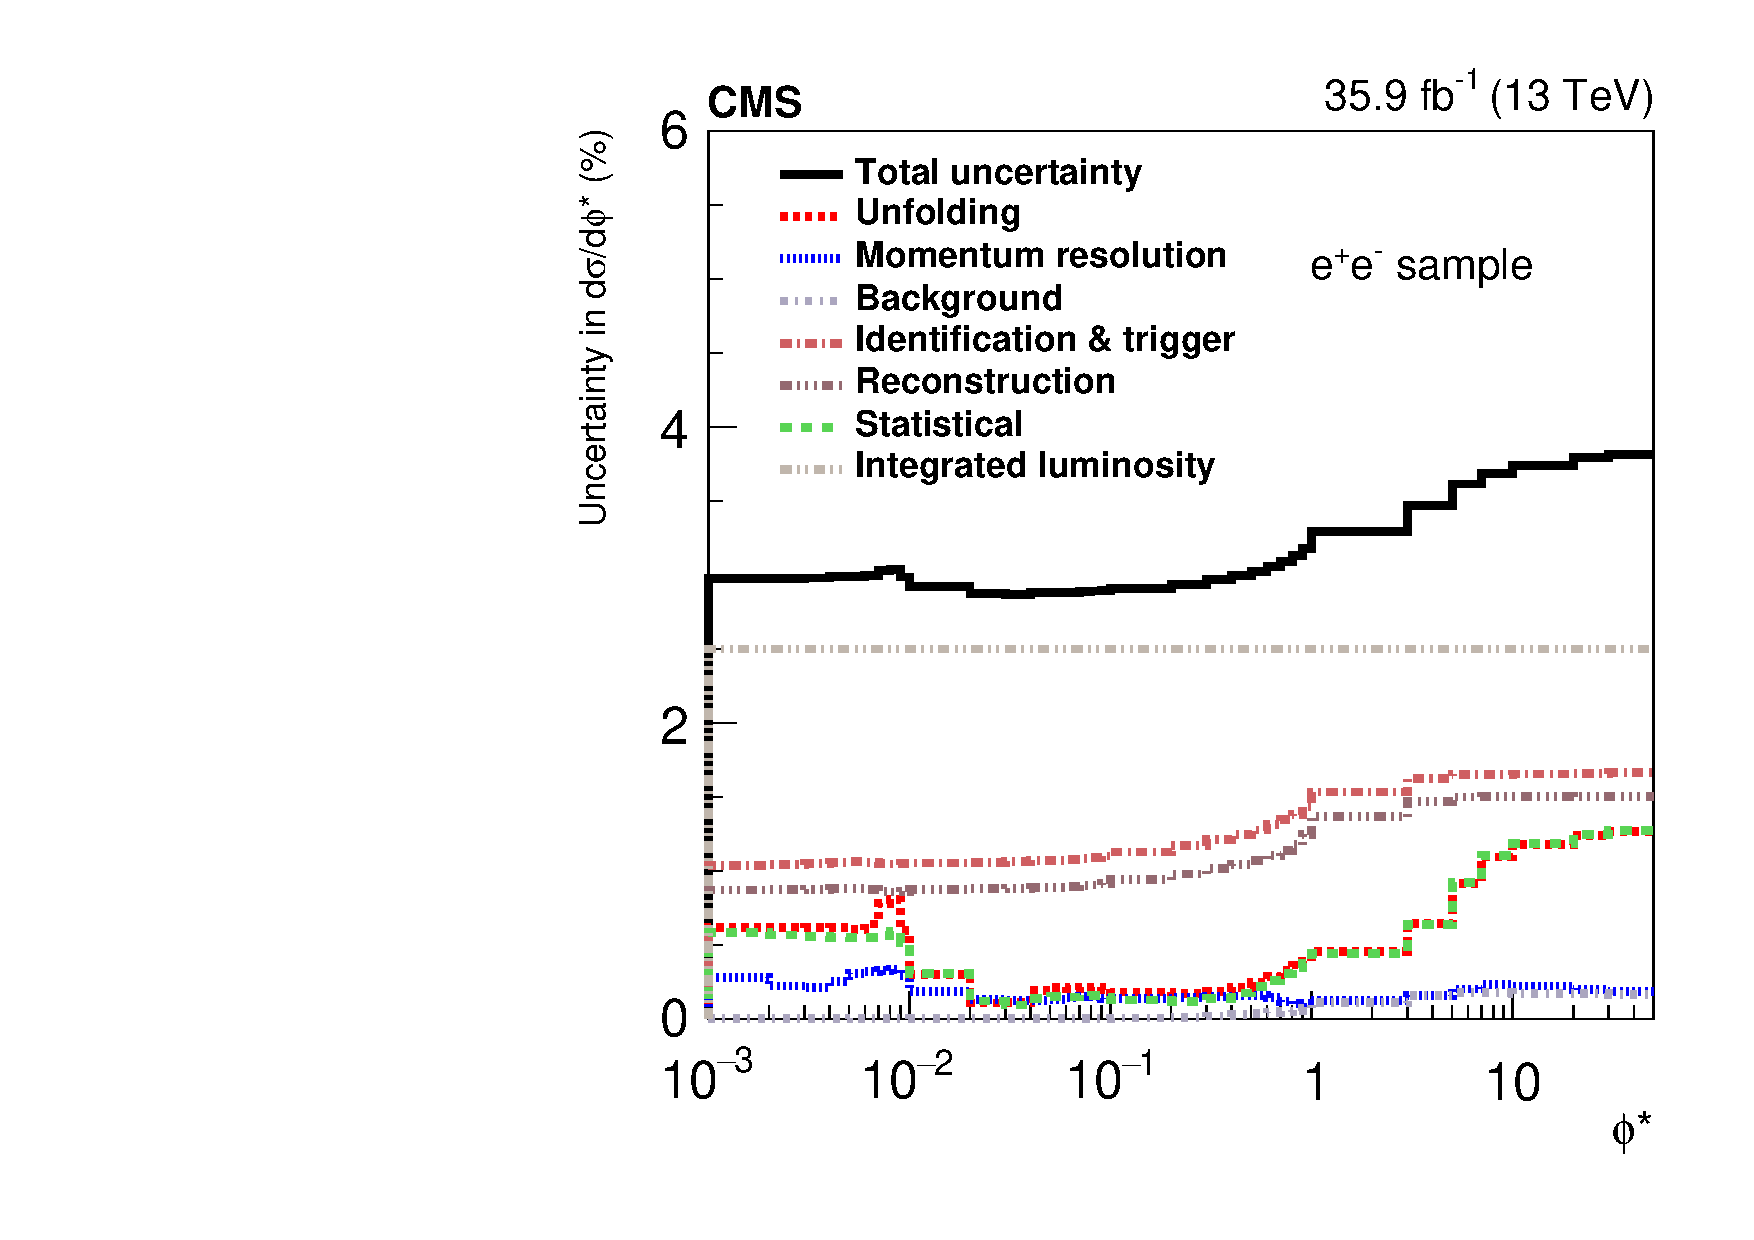
\includegraphics[width=0.49\textwidth]{figures/zpt/histoUnfoldingSystPhiStar_nsel1_dy3.pdf}
	\caption{Summary of the systematic uncertainties of muons (left) and electrons (right) 
	for the $\pt^{\Z}$ analysis (top), the $|\rapidity^\Z|$ analysis (center), and the $\phi^\star$ analysis (bottom).}
	\label{fig:zpt_syst0}
\end{figure}

\begin{figure}
	\centering
	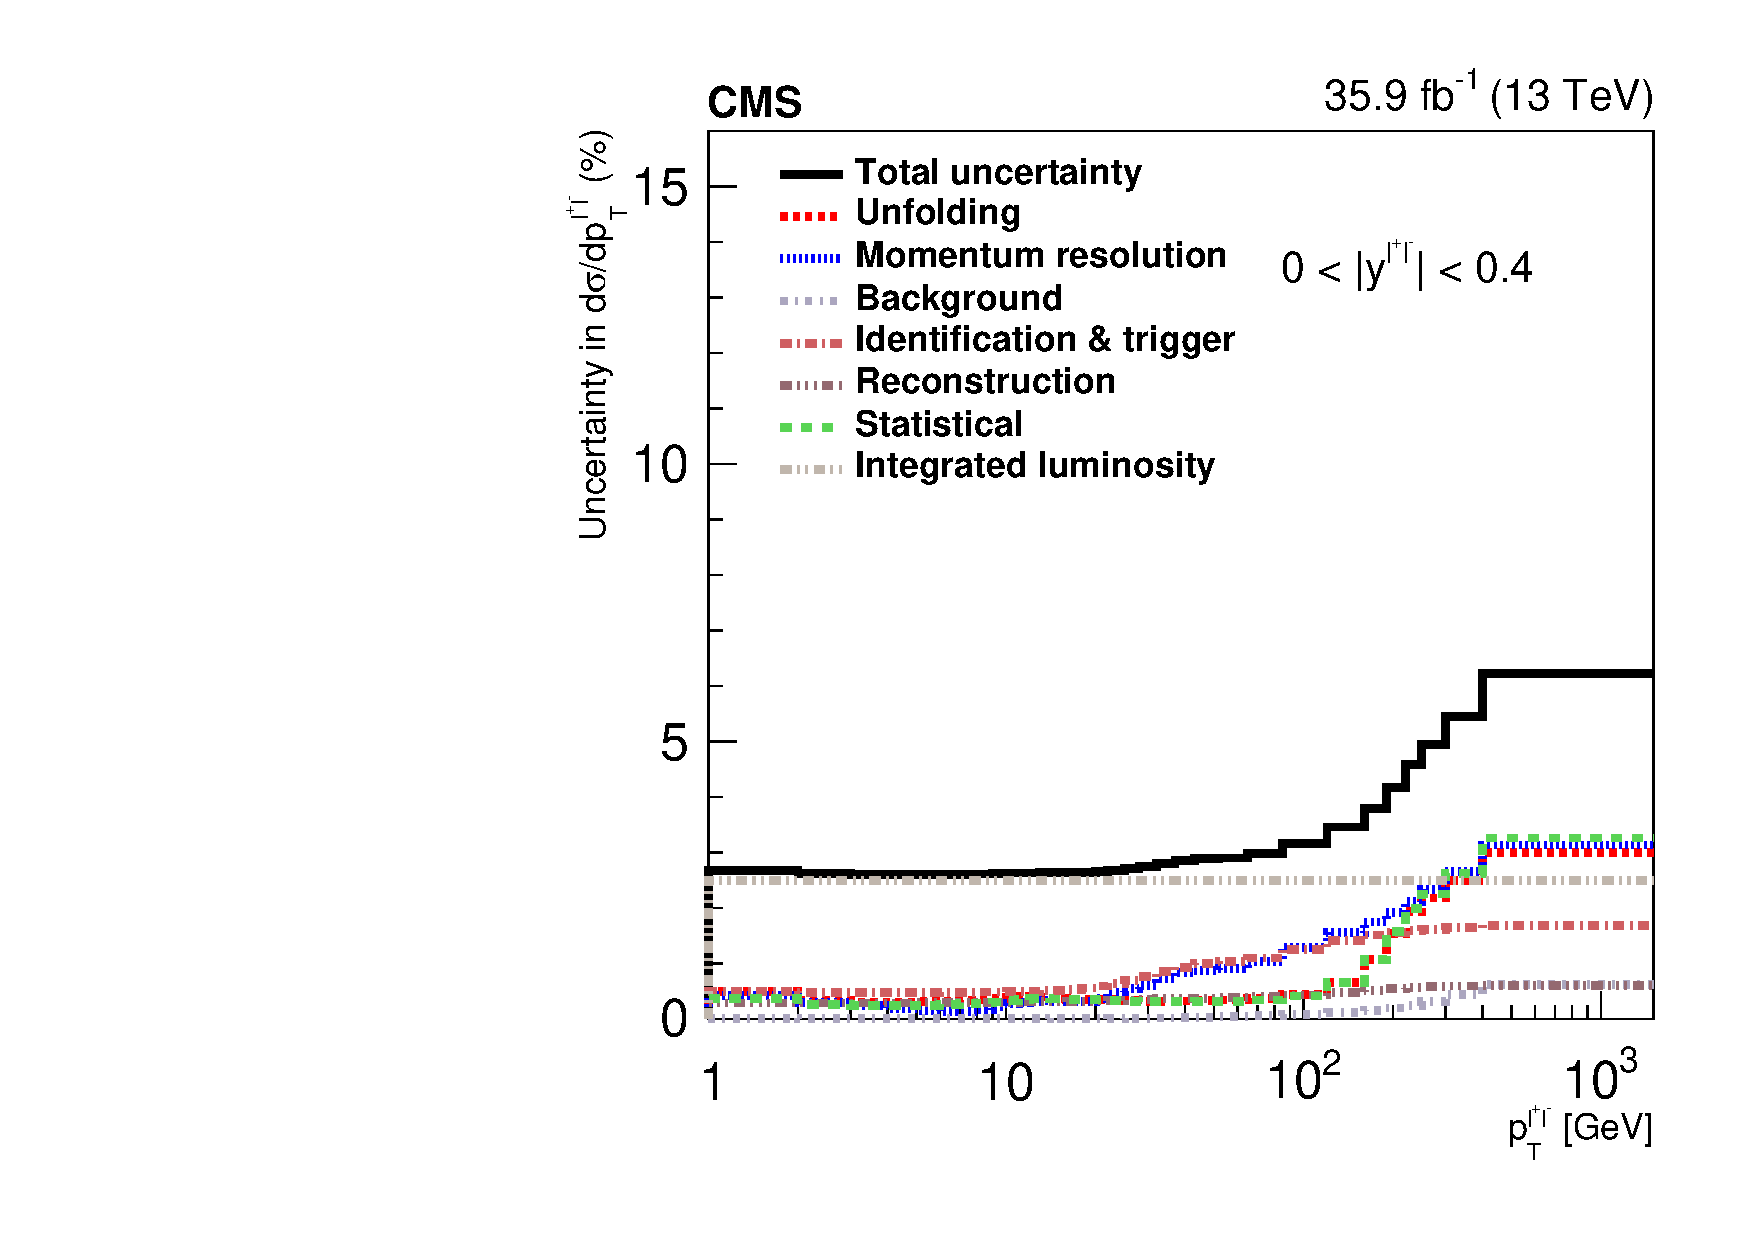
\includegraphics[width=0.49\textwidth]{figures/zpt/histoUnfoldingSystPtRap0_nsel0_dy3.pdf}
	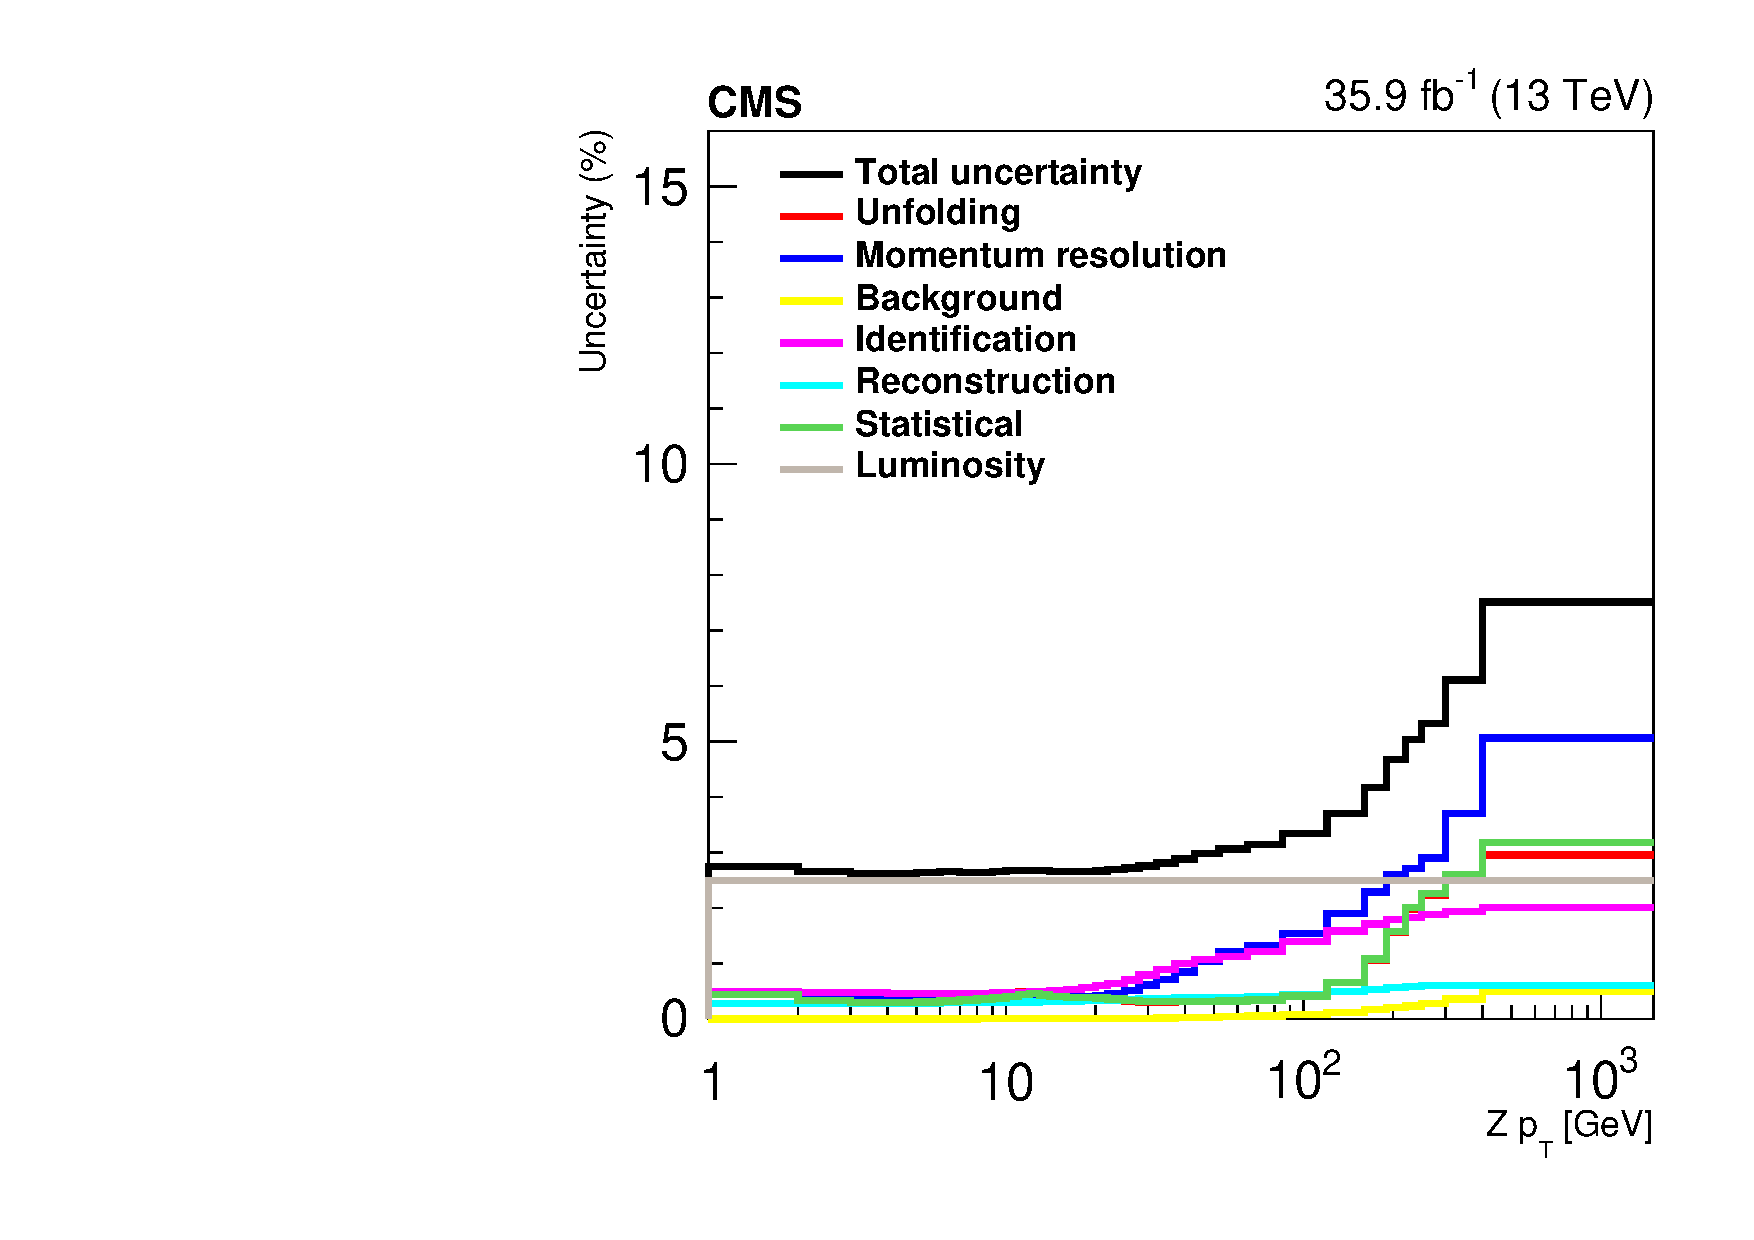
\includegraphics[width=0.49\textwidth]{figures/zpt/histoUnfoldingSystPtRap1_nsel0_dy3.pdf}
	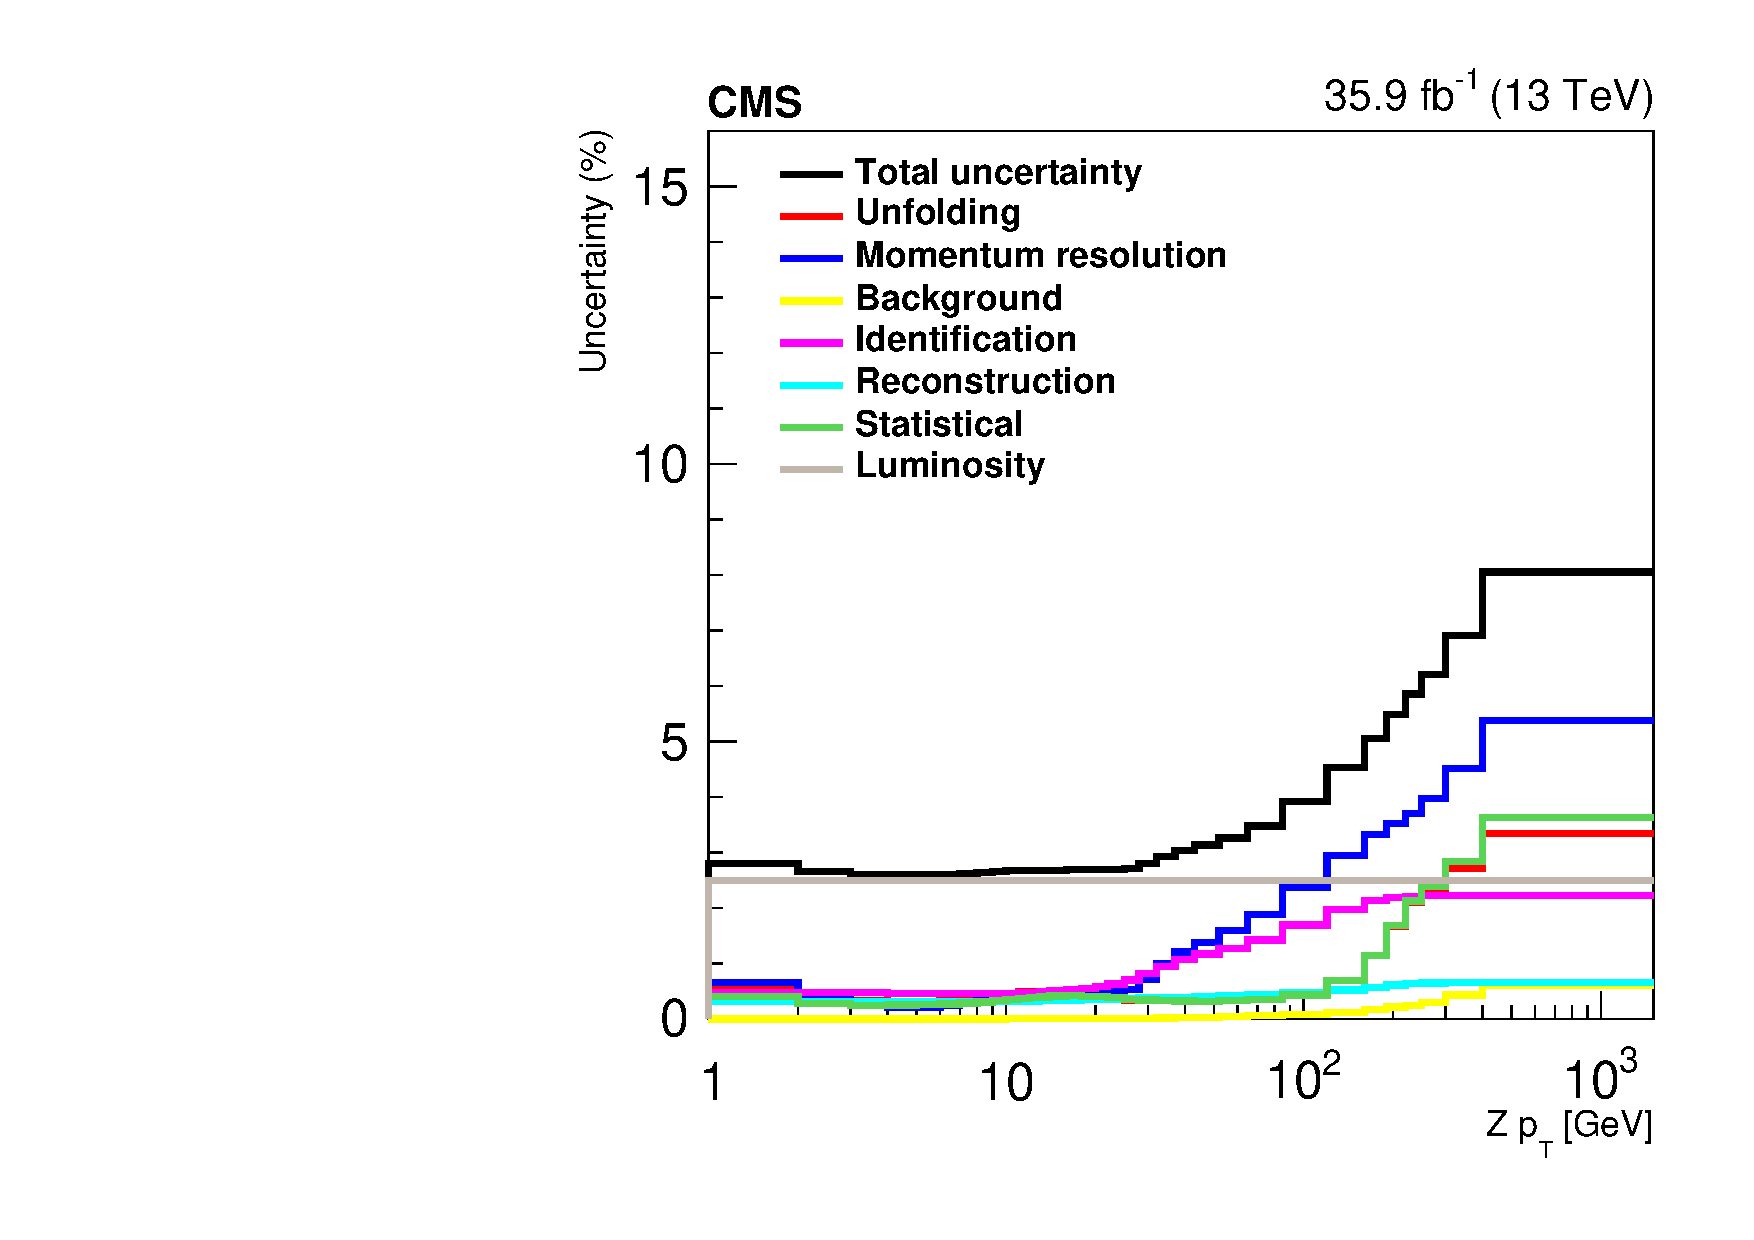
\includegraphics[width=0.49\textwidth]{figures/zpt/histoUnfoldingSystPtRap2_nsel0_dy3.pdf}
	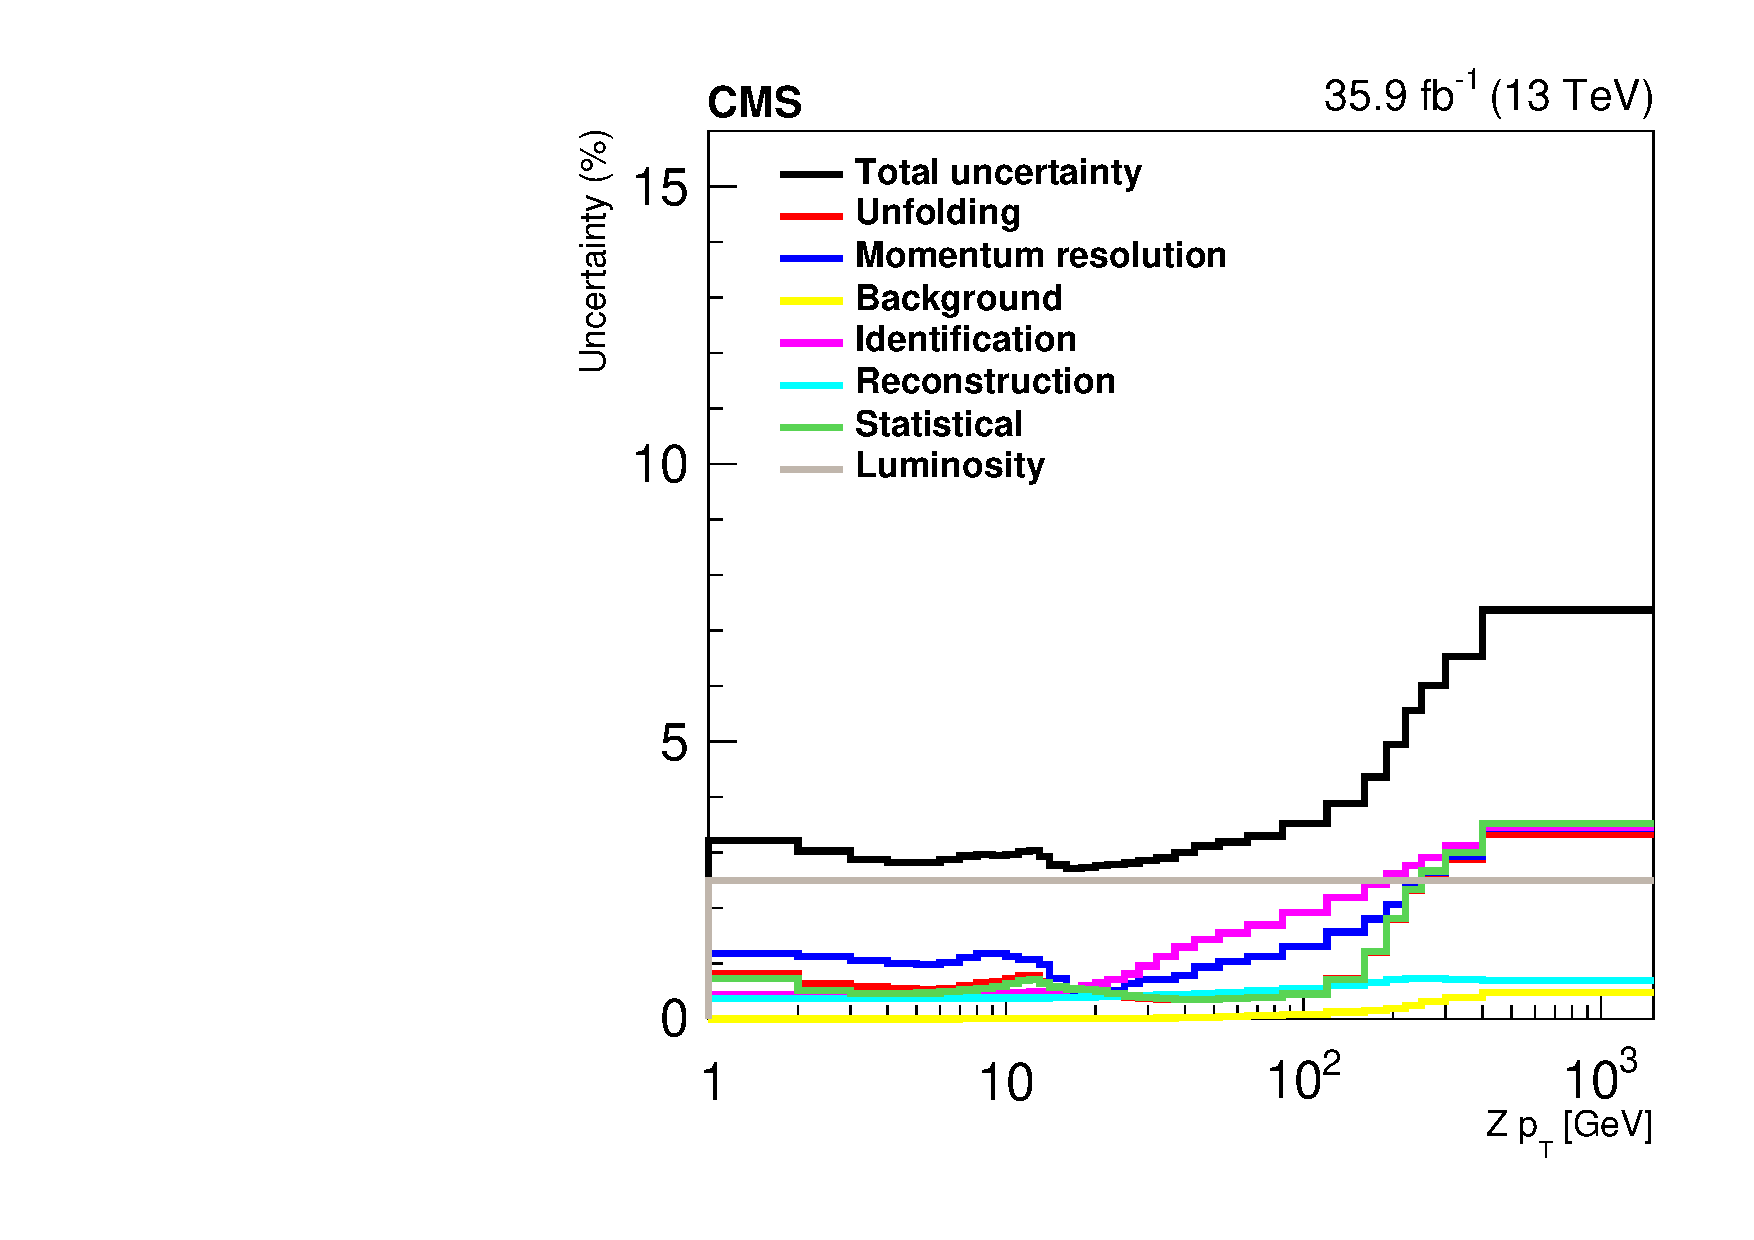
\includegraphics[width=0.49\textwidth]{figures/zpt/histoUnfoldingSystPtRap3_nsel0_dy3.pdf}
	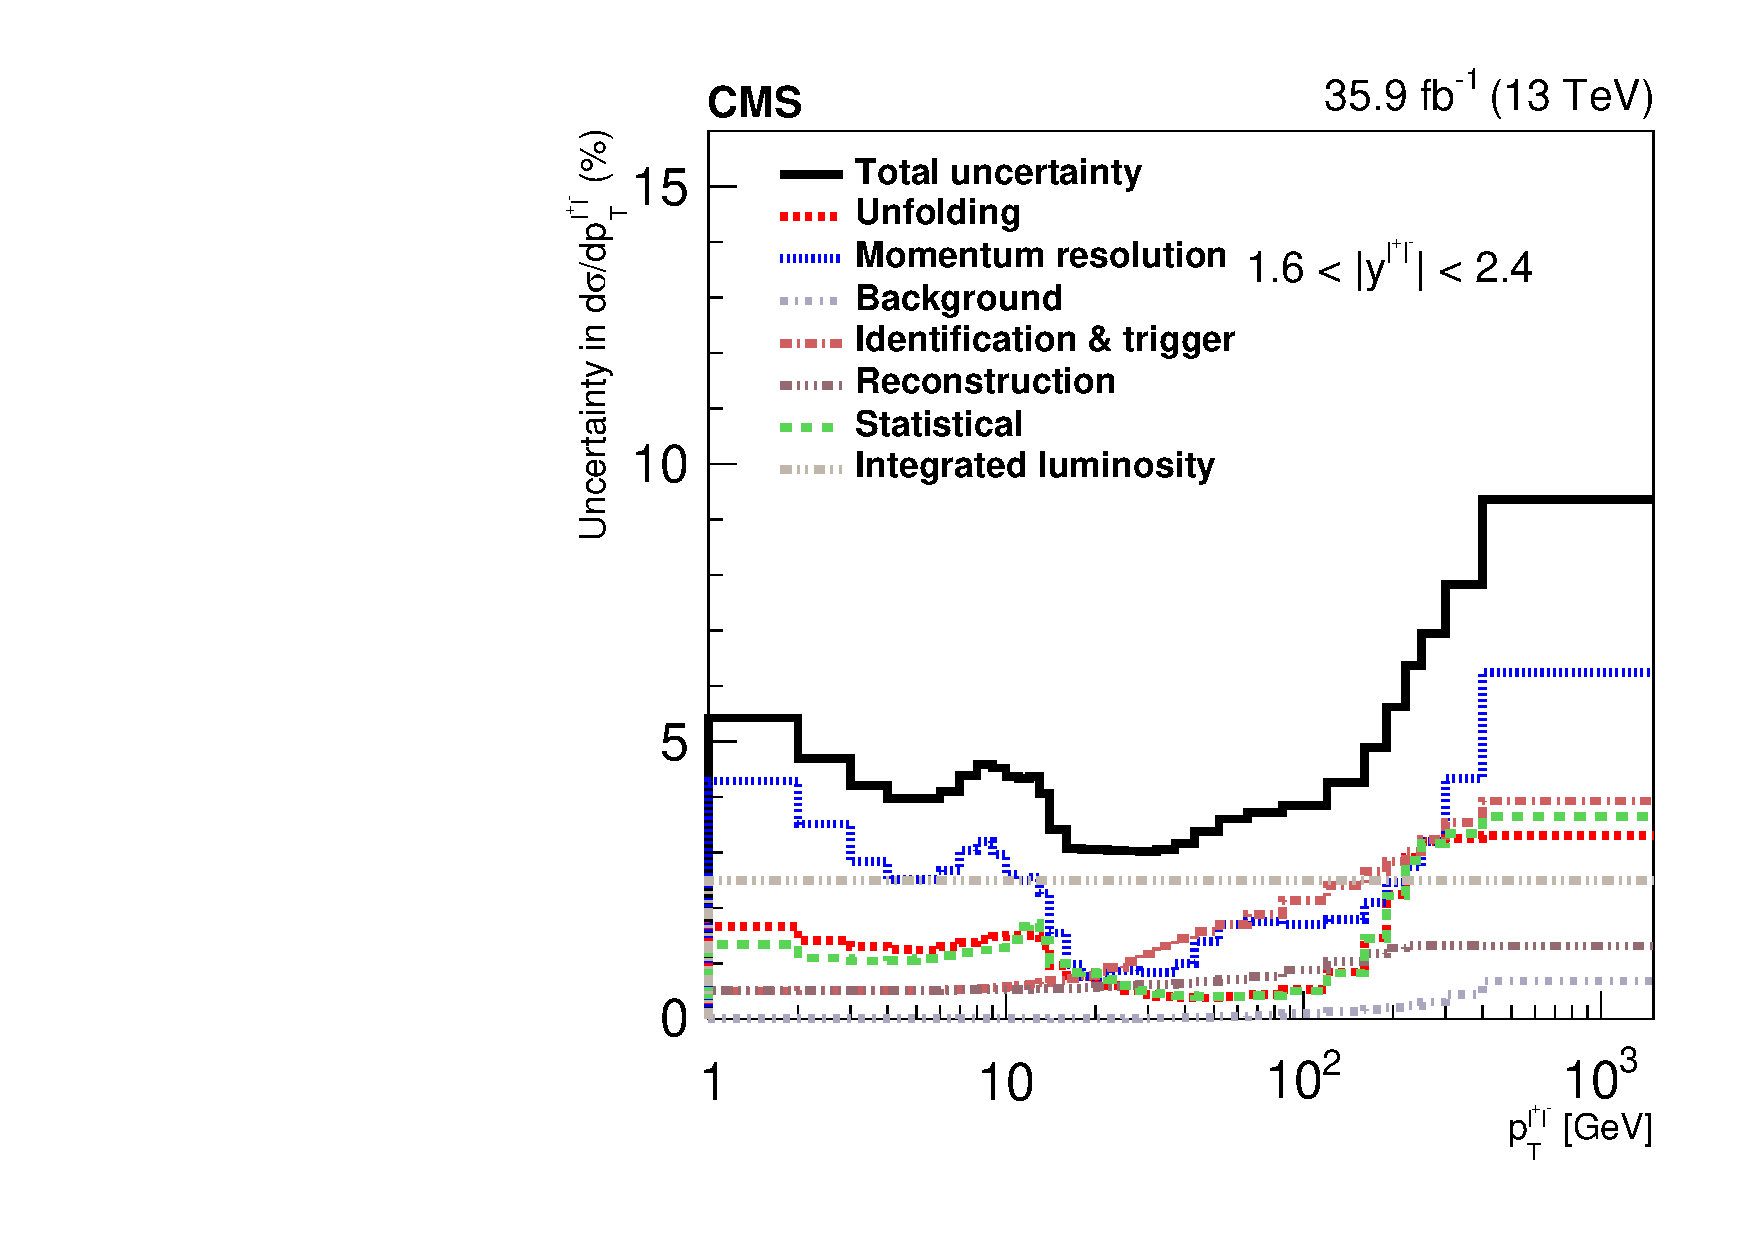
\includegraphics[width=0.49\textwidth]{figures/zpt/histoUnfoldingSystPtRap4_nsel0_dy3.pdf}
	\caption{Summary of the systematic uncertainties for the $\pt^{\Z}$ analysis of muons in the 
	$0.0 < |\rapidity^\Z| < 0.4$ region (top left), $0.4 < |\rapidity^\Z| < 0.8$ region (top right),
	$0.8 < |\rapidity^\Z| < 1.2$ region (center left), $1.2 < |\rapidity^\Z| < 1.6$ region (center right), and 
	$1.6 < |\rapidity^\Z| < 2,4$ region (bottom).
	}
	\label{fig:zpt_syst1}
\end{figure}

\begin{figure}
	\centering
	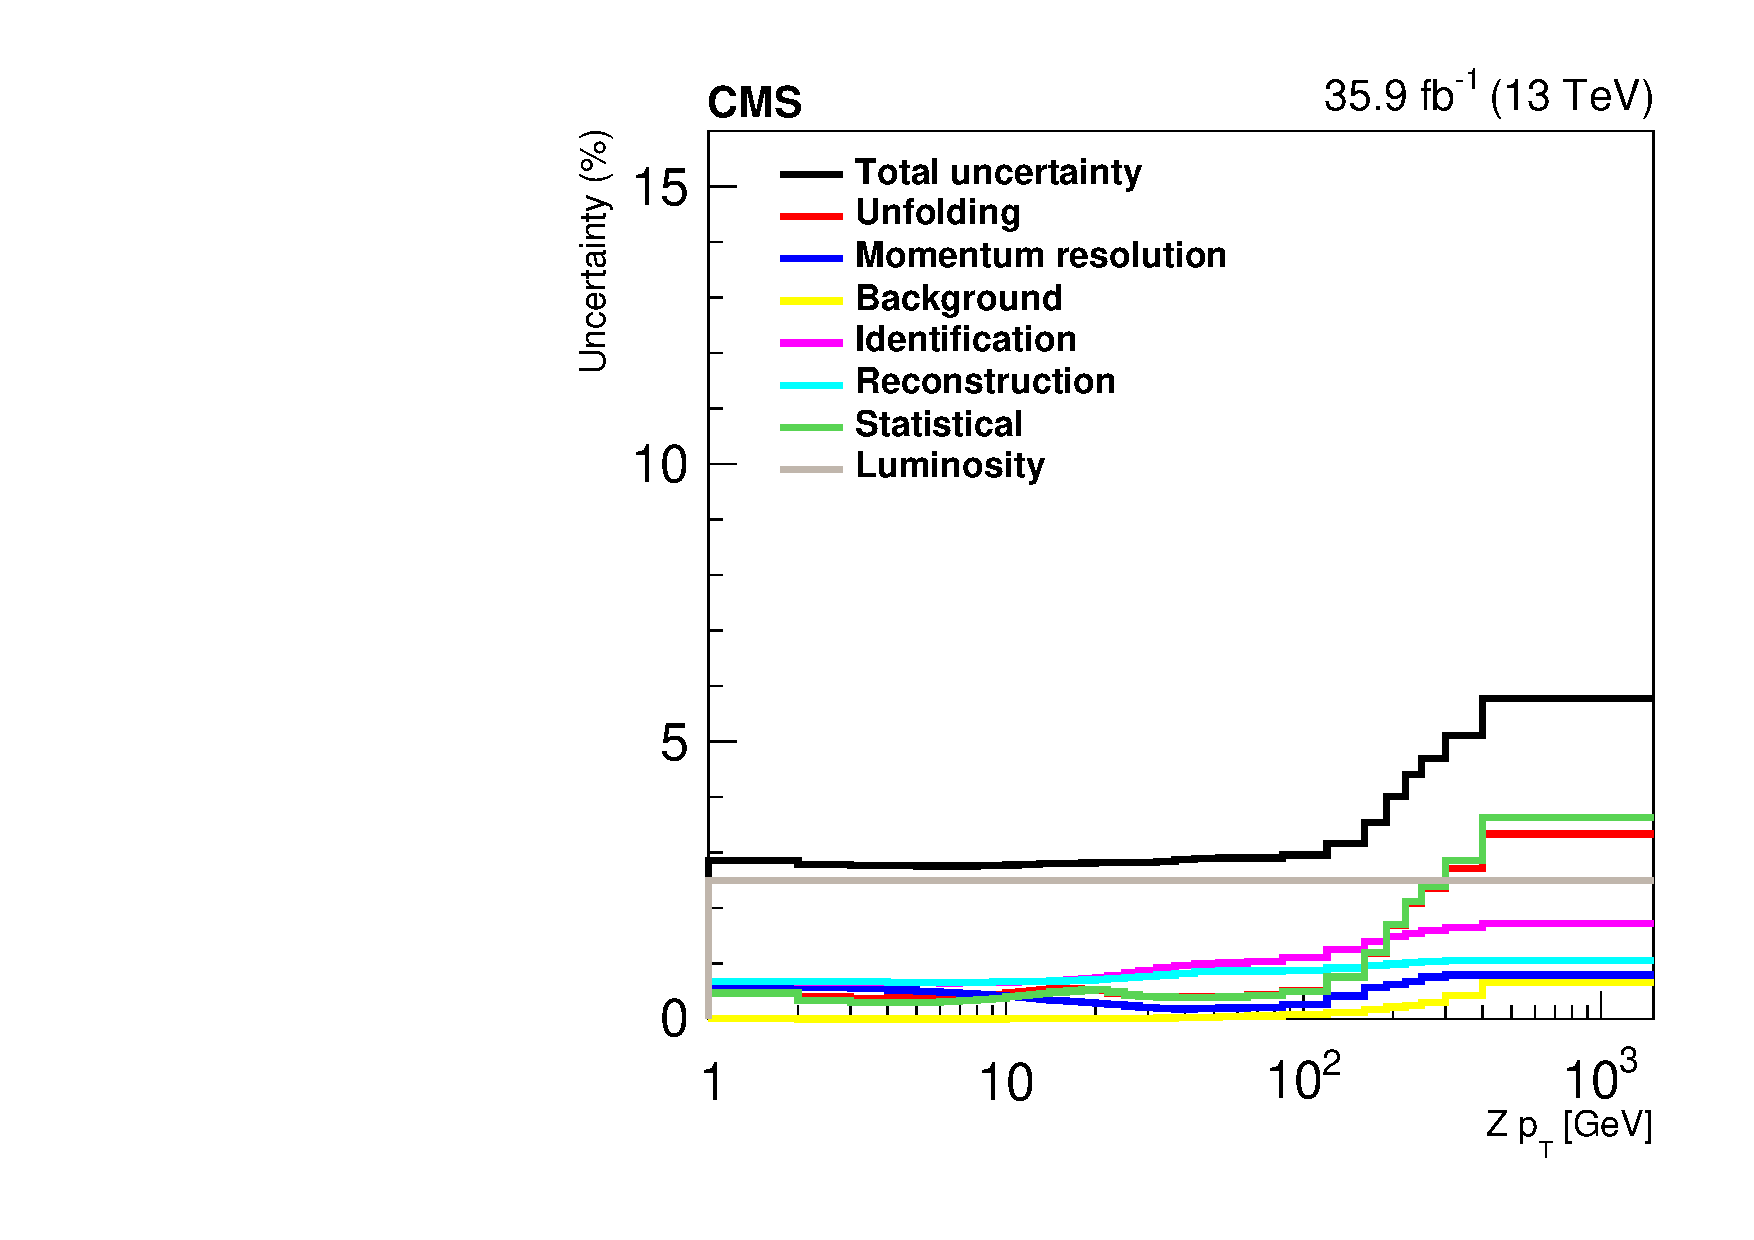
\includegraphics[width=0.49\textwidth]{figures/zpt/histoUnfoldingSystPtRap0_nsel1_dy3.pdf}
	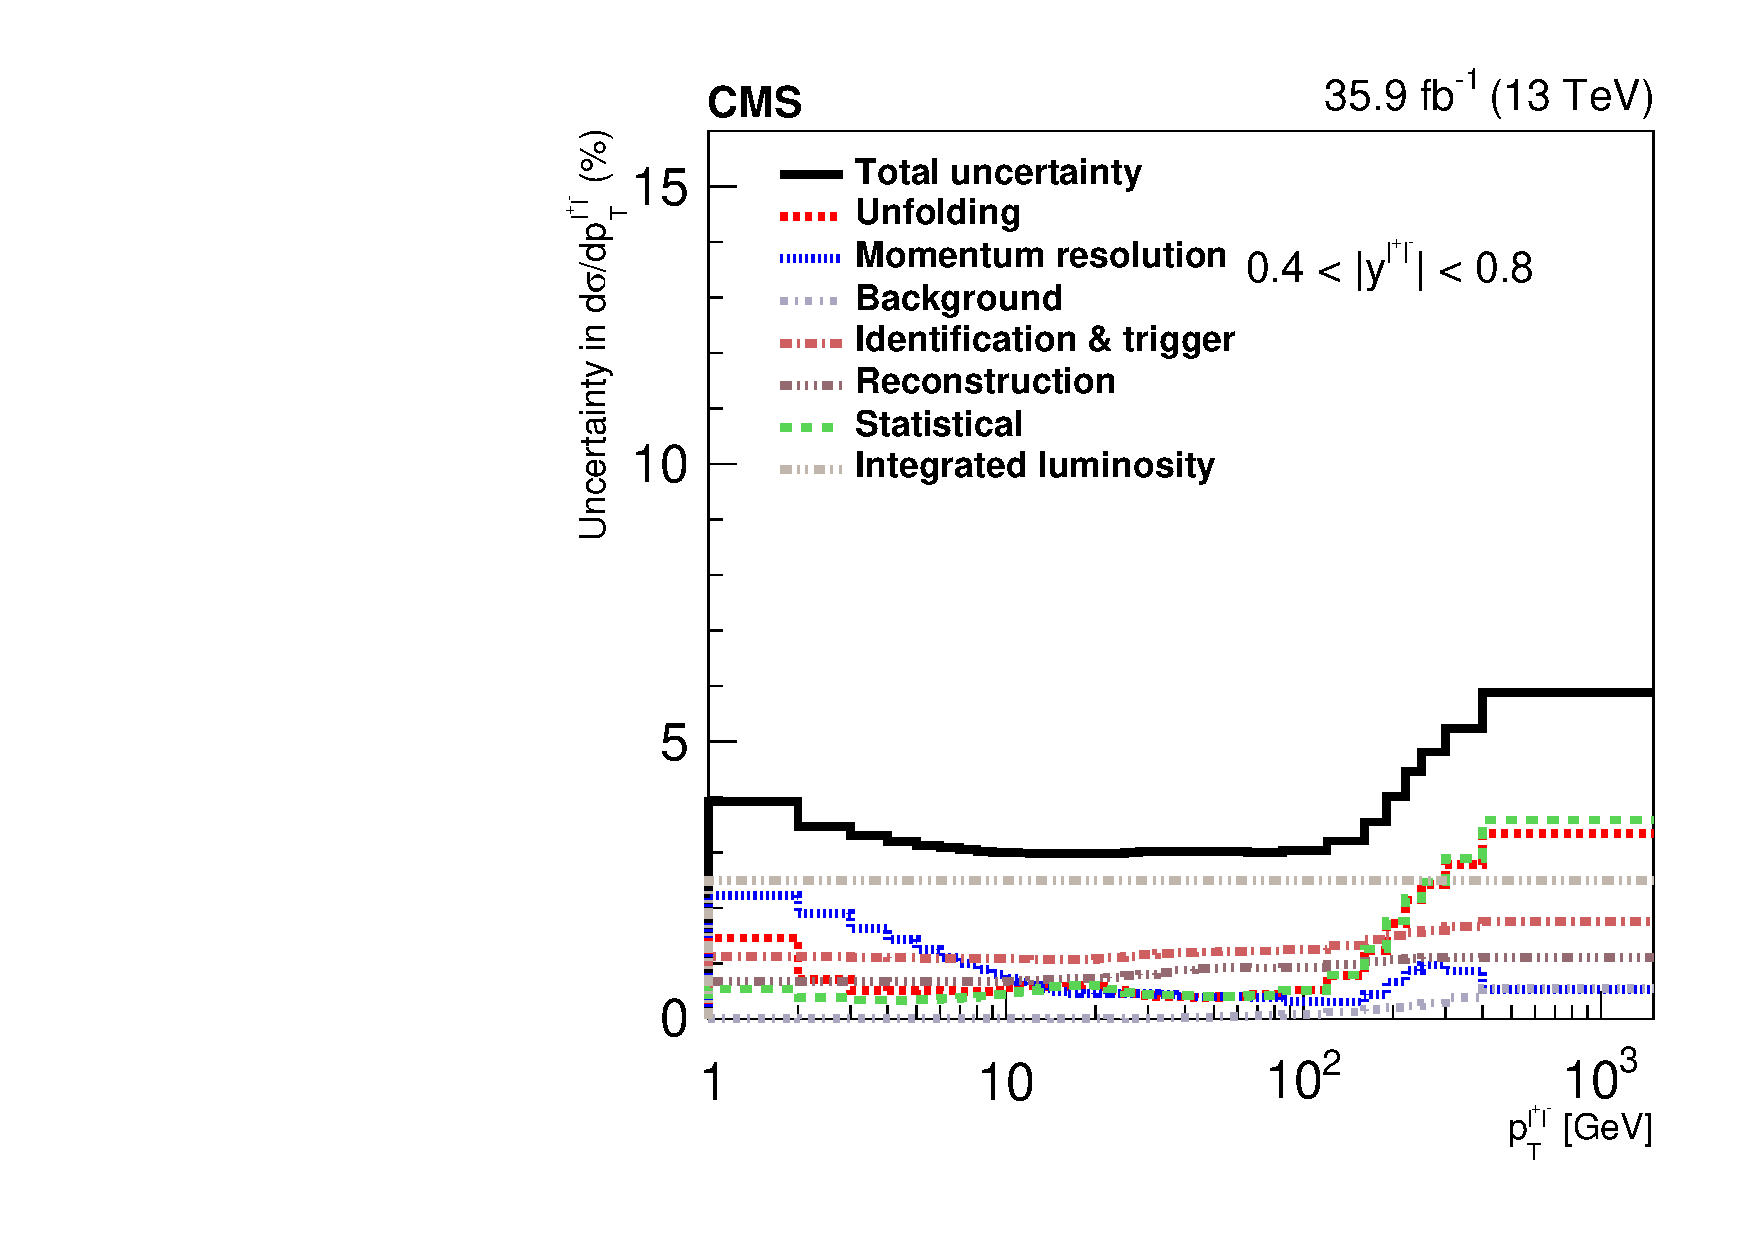
\includegraphics[width=0.49\textwidth]{figures/zpt/histoUnfoldingSystPtRap1_nsel1_dy3.pdf}
	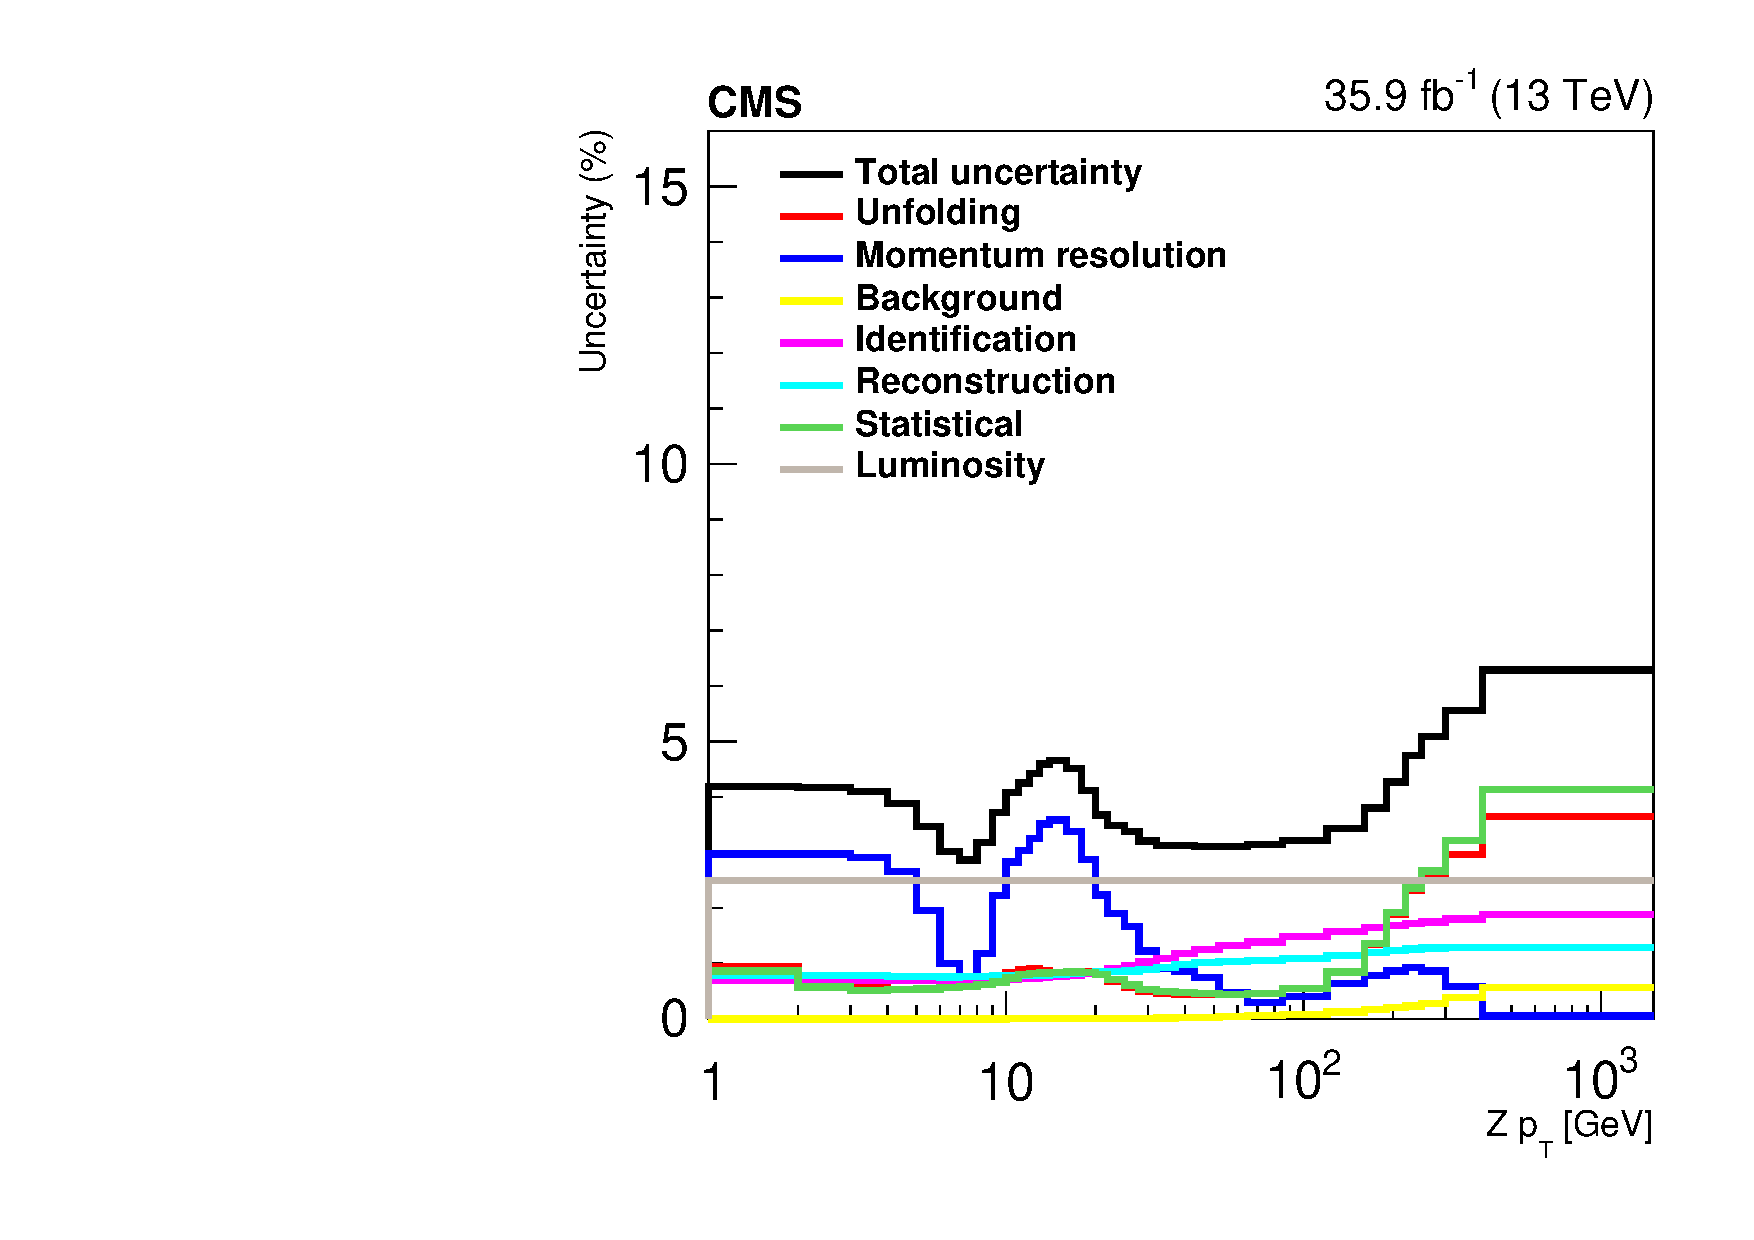
\includegraphics[width=0.49\textwidth]{figures/zpt/histoUnfoldingSystPtRap2_nsel1_dy3.pdf}
	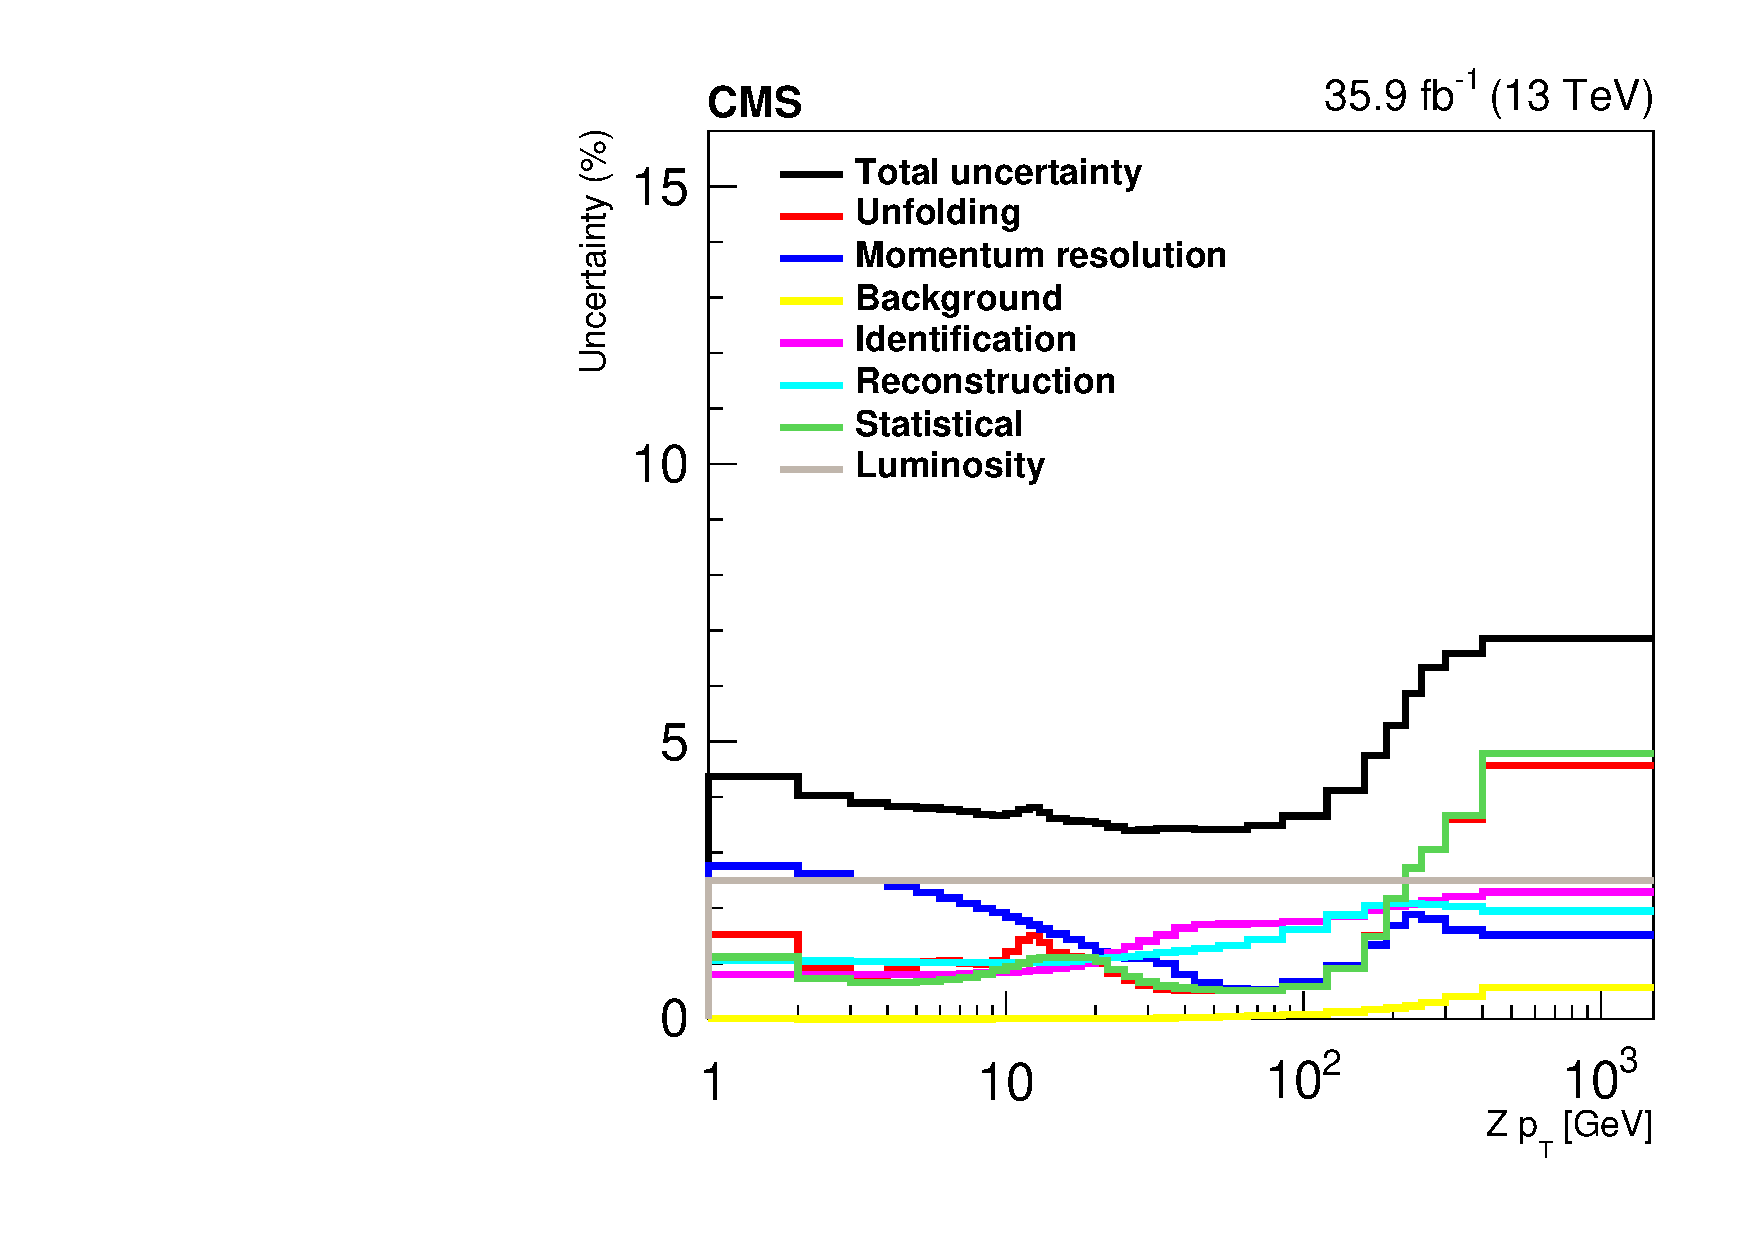
\includegraphics[width=0.49\textwidth]{figures/zpt/histoUnfoldingSystPtRap3_nsel1_dy3.pdf}
	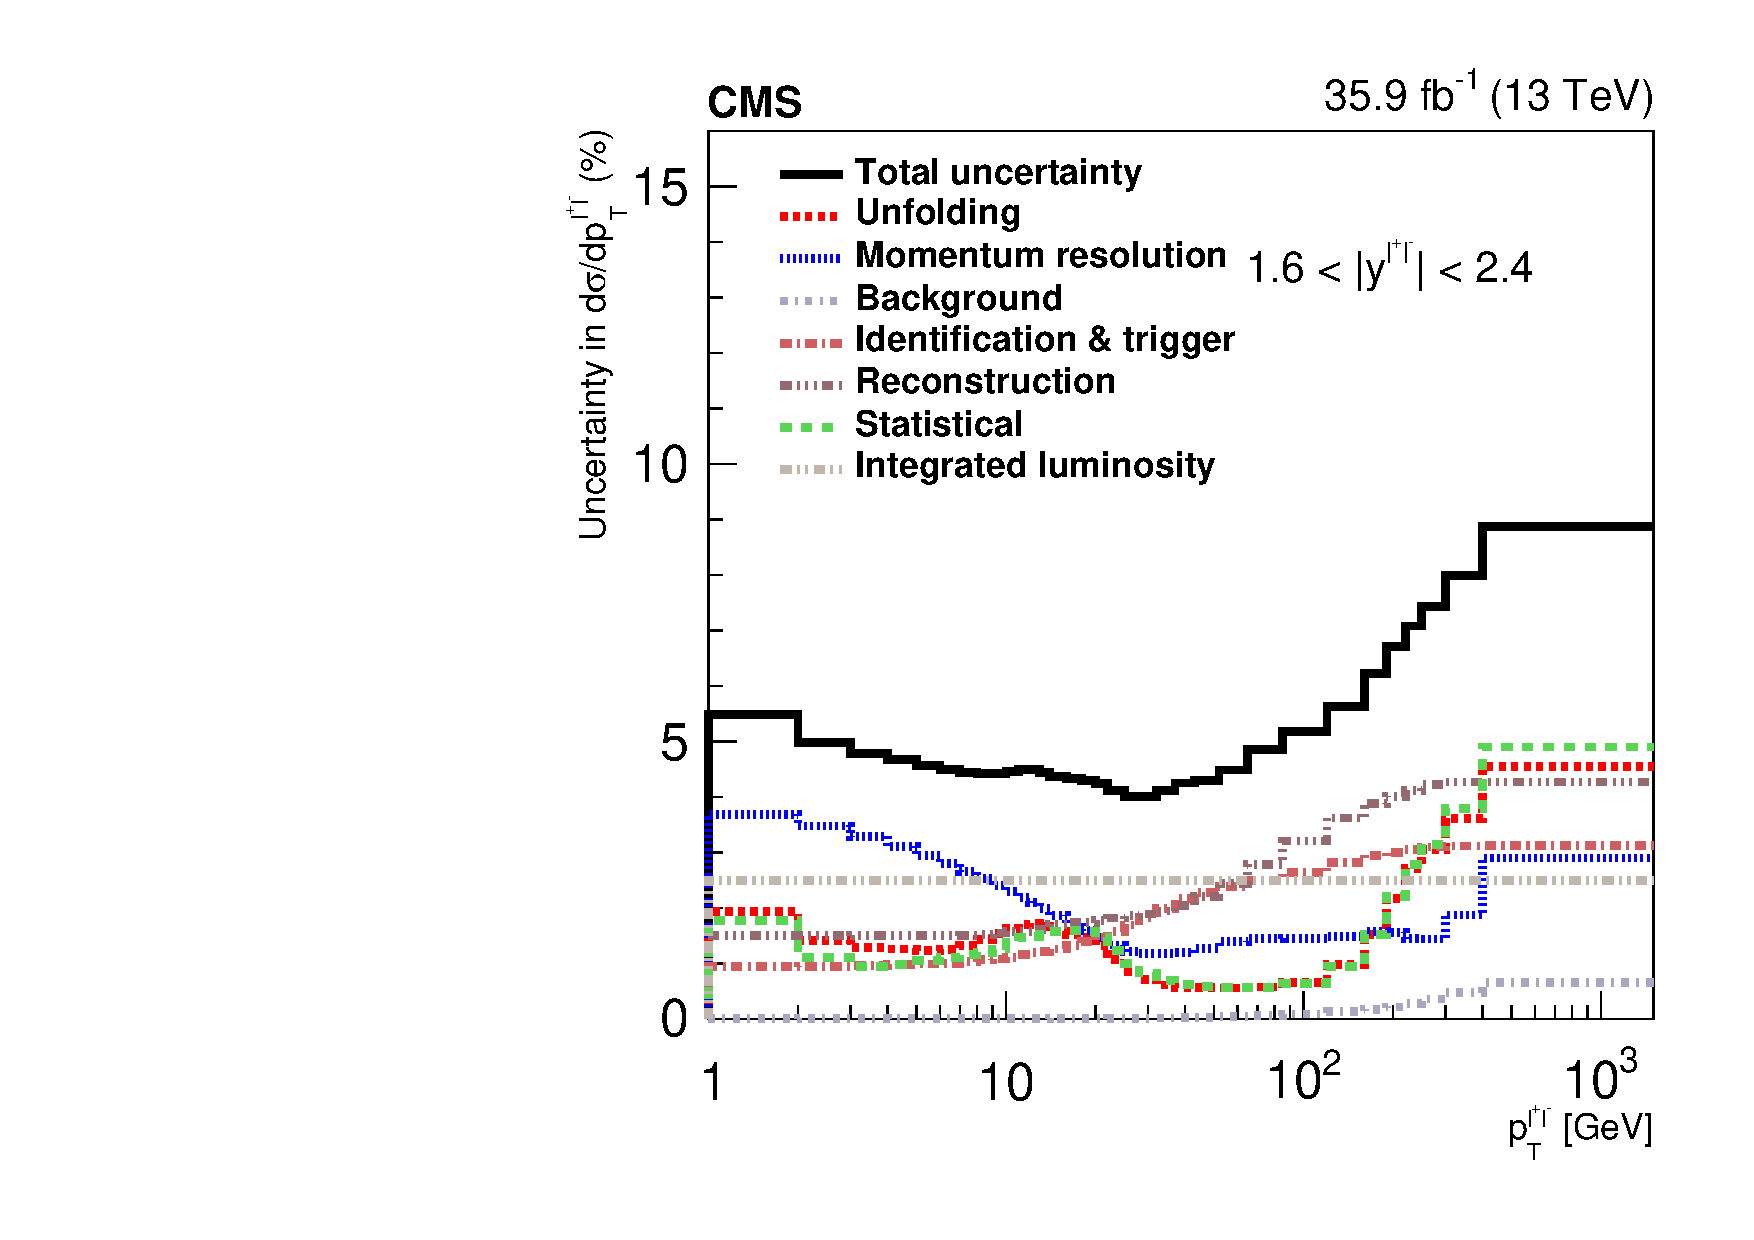
\includegraphics[width=0.49\textwidth]{figures/zpt/histoUnfoldingSystPtRap4_nsel1_dy3.pdf}
	\caption{Summary of the systematic uncertainties for the $\pt^{\Z}$ analysis of electrons in the 
	$0.0 < |\rapidity^\Z| < 0.4$ region (top left), $0.4 < |\rapidity^\Z| < 0.8$ region (top right),
	$0.8 < |\rapidity^\Z| < 1.2$ region (center left), $1.2 < |\rapidity^\Z| < 1.6$ region (center right), and 
	$1.6 < |\rapidity^\Z| < 2,4$ region (bottom).
	}
	\label{fig:zpt_syst2}
\end{figure}

\begin{figure}
	\centering
	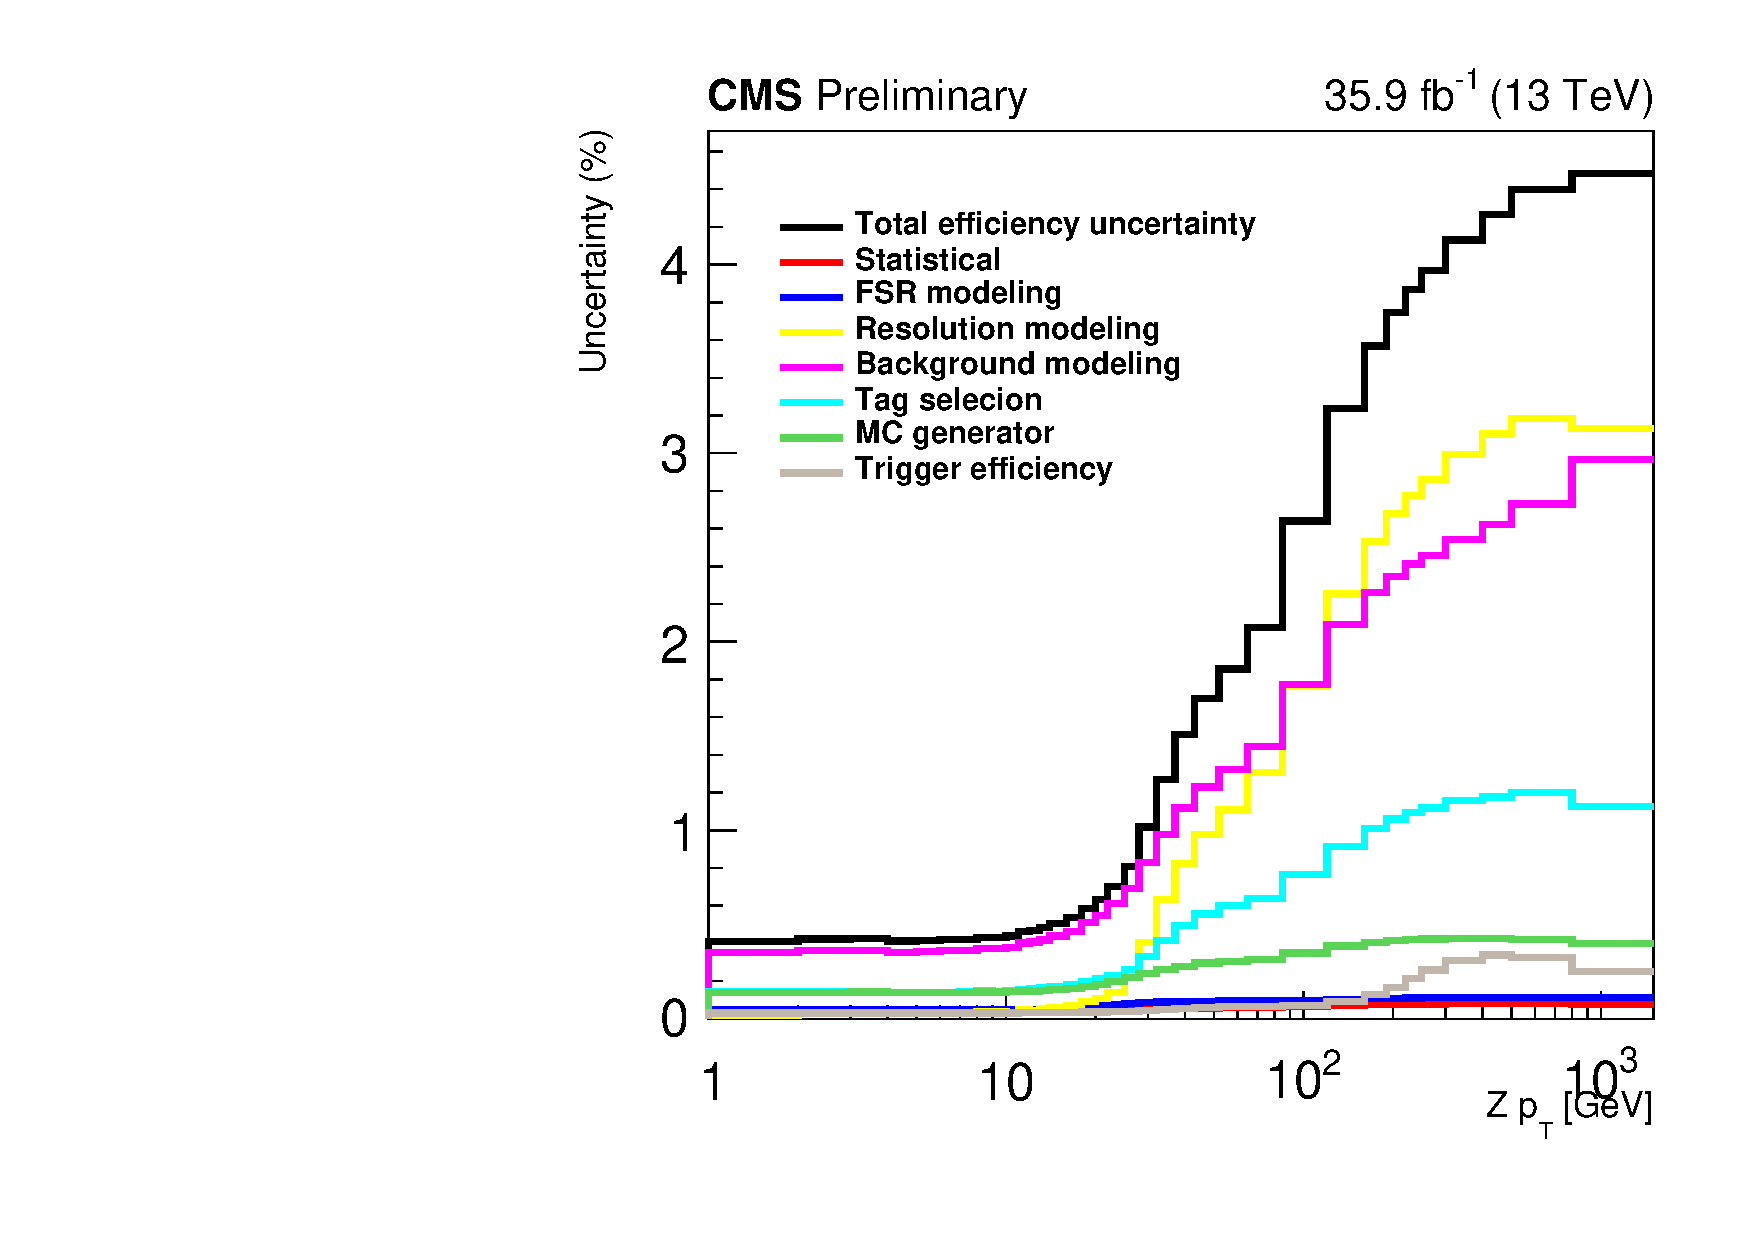
\includegraphics[width=0.49\textwidth]{figures/zpt/histoUnfoldingSystEffPt_nsel0_dy3.pdf}
        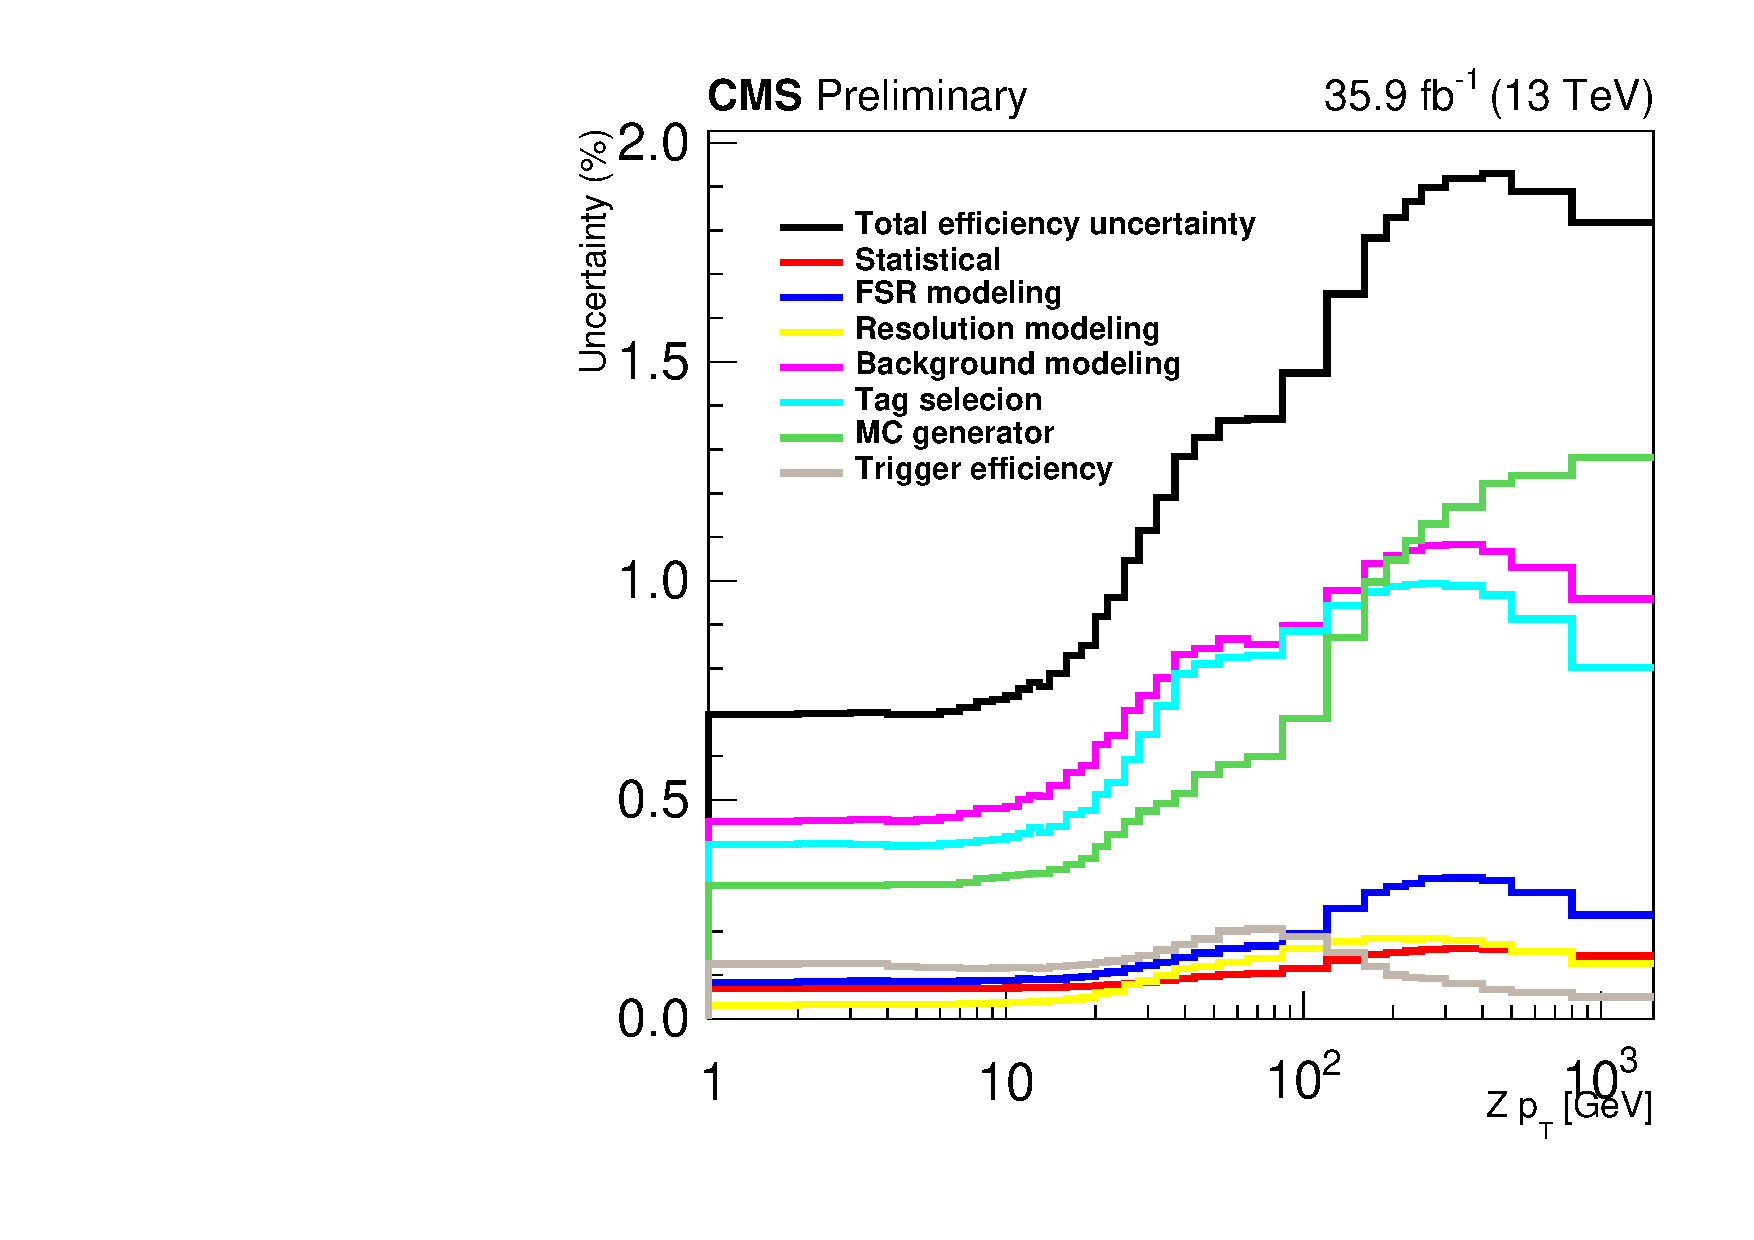
\includegraphics[width=0.49\textwidth]{figures/zpt/histoUnfoldingSystEffPt_nsel1_dy3.pdf}
	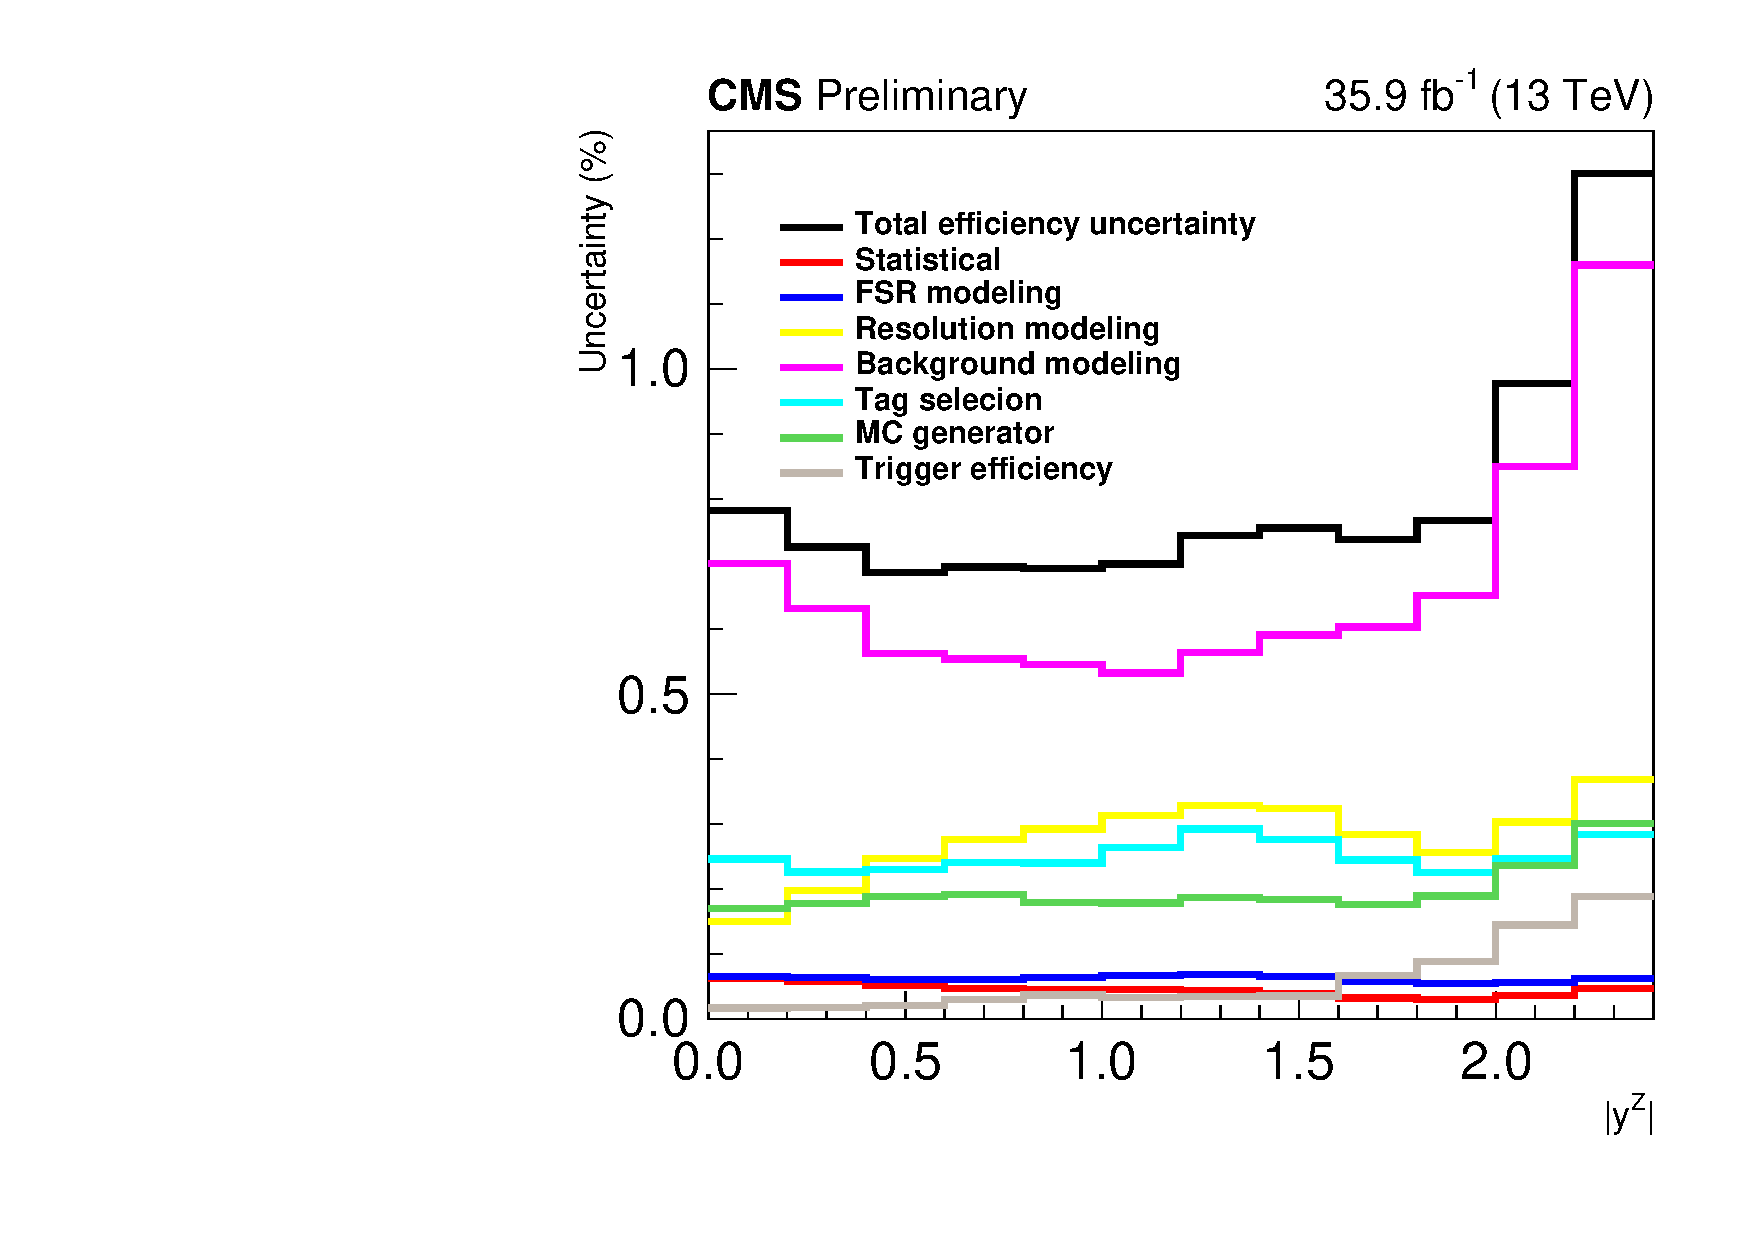
\includegraphics[width=0.49\textwidth]{figures/zpt/histoUnfoldingSystEffRap_nsel0_dy3.pdf}
        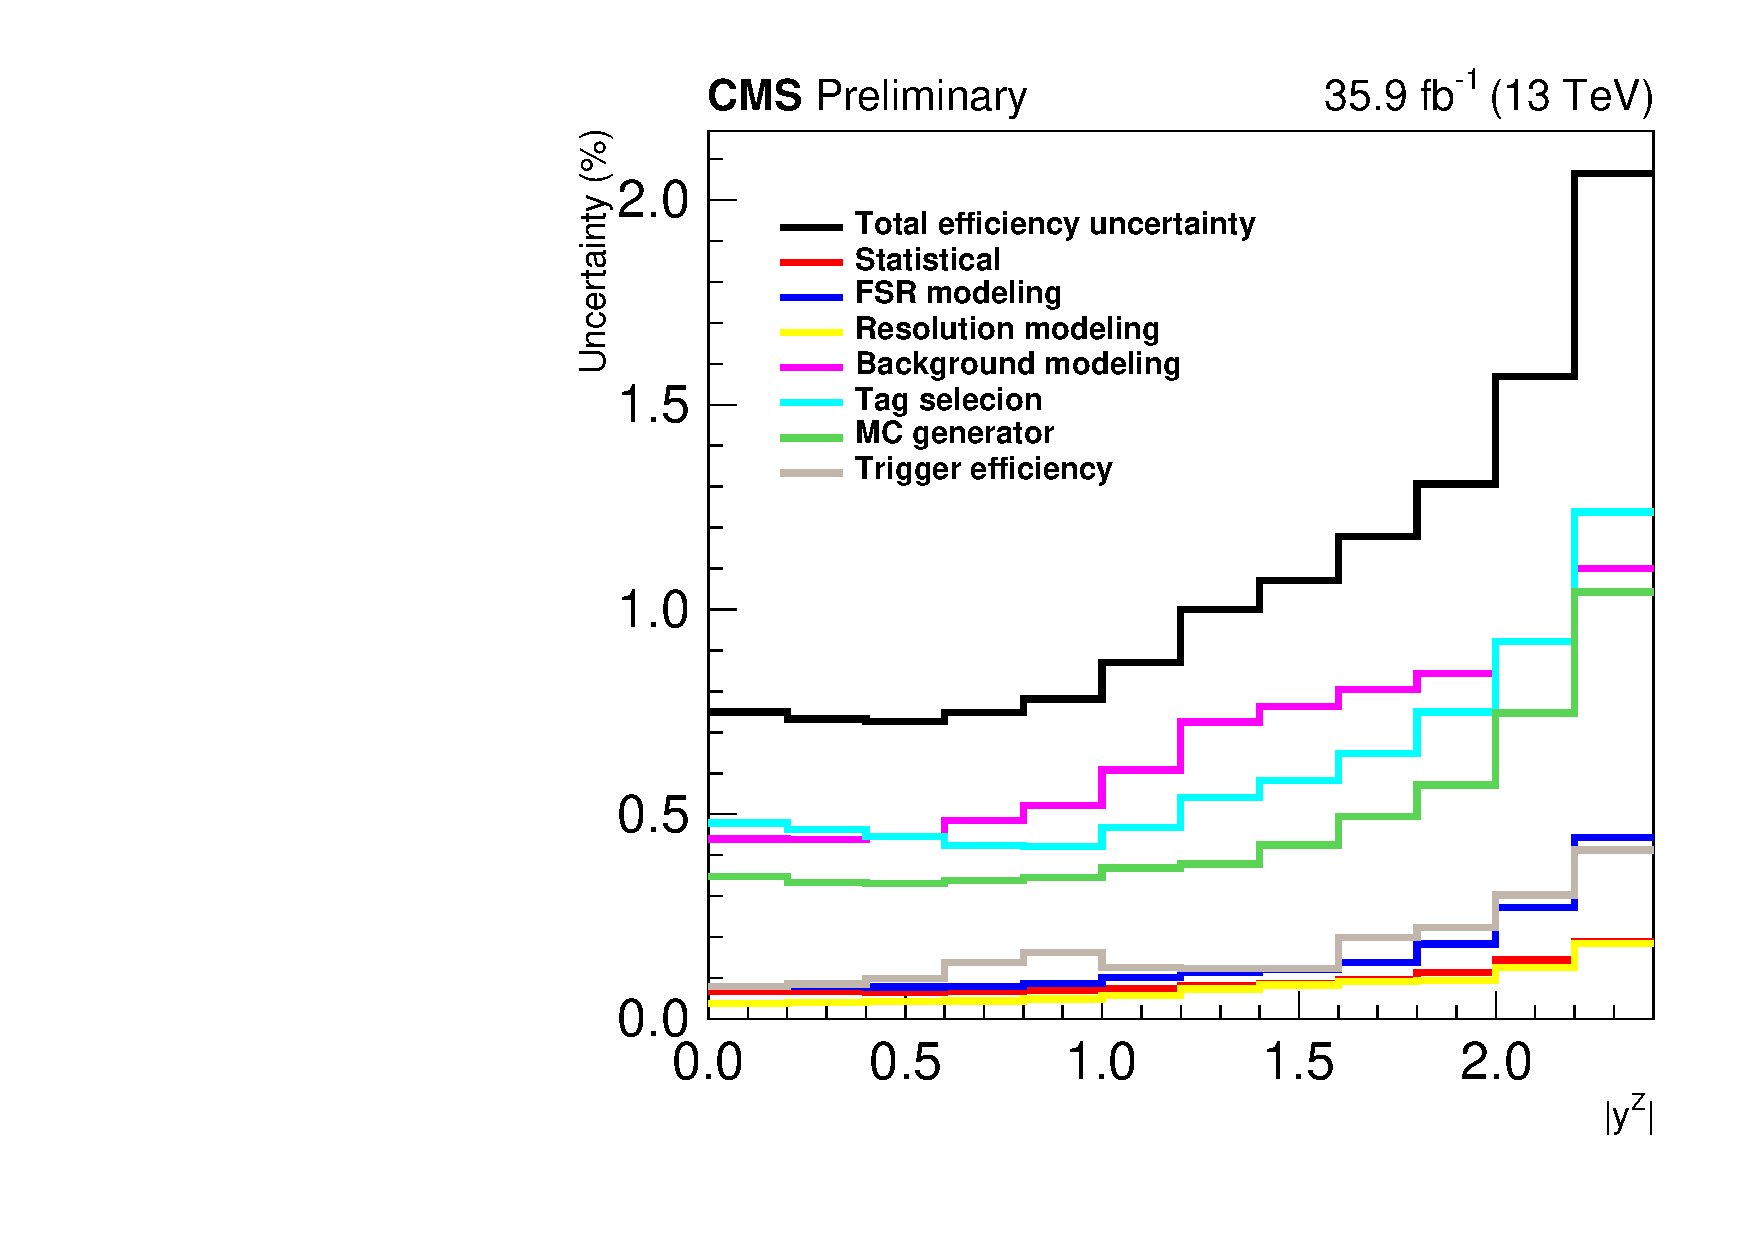
\includegraphics[width=0.49\textwidth]{figures/zpt/histoUnfoldingSystEffRap_nsel1_dy3.pdf}
	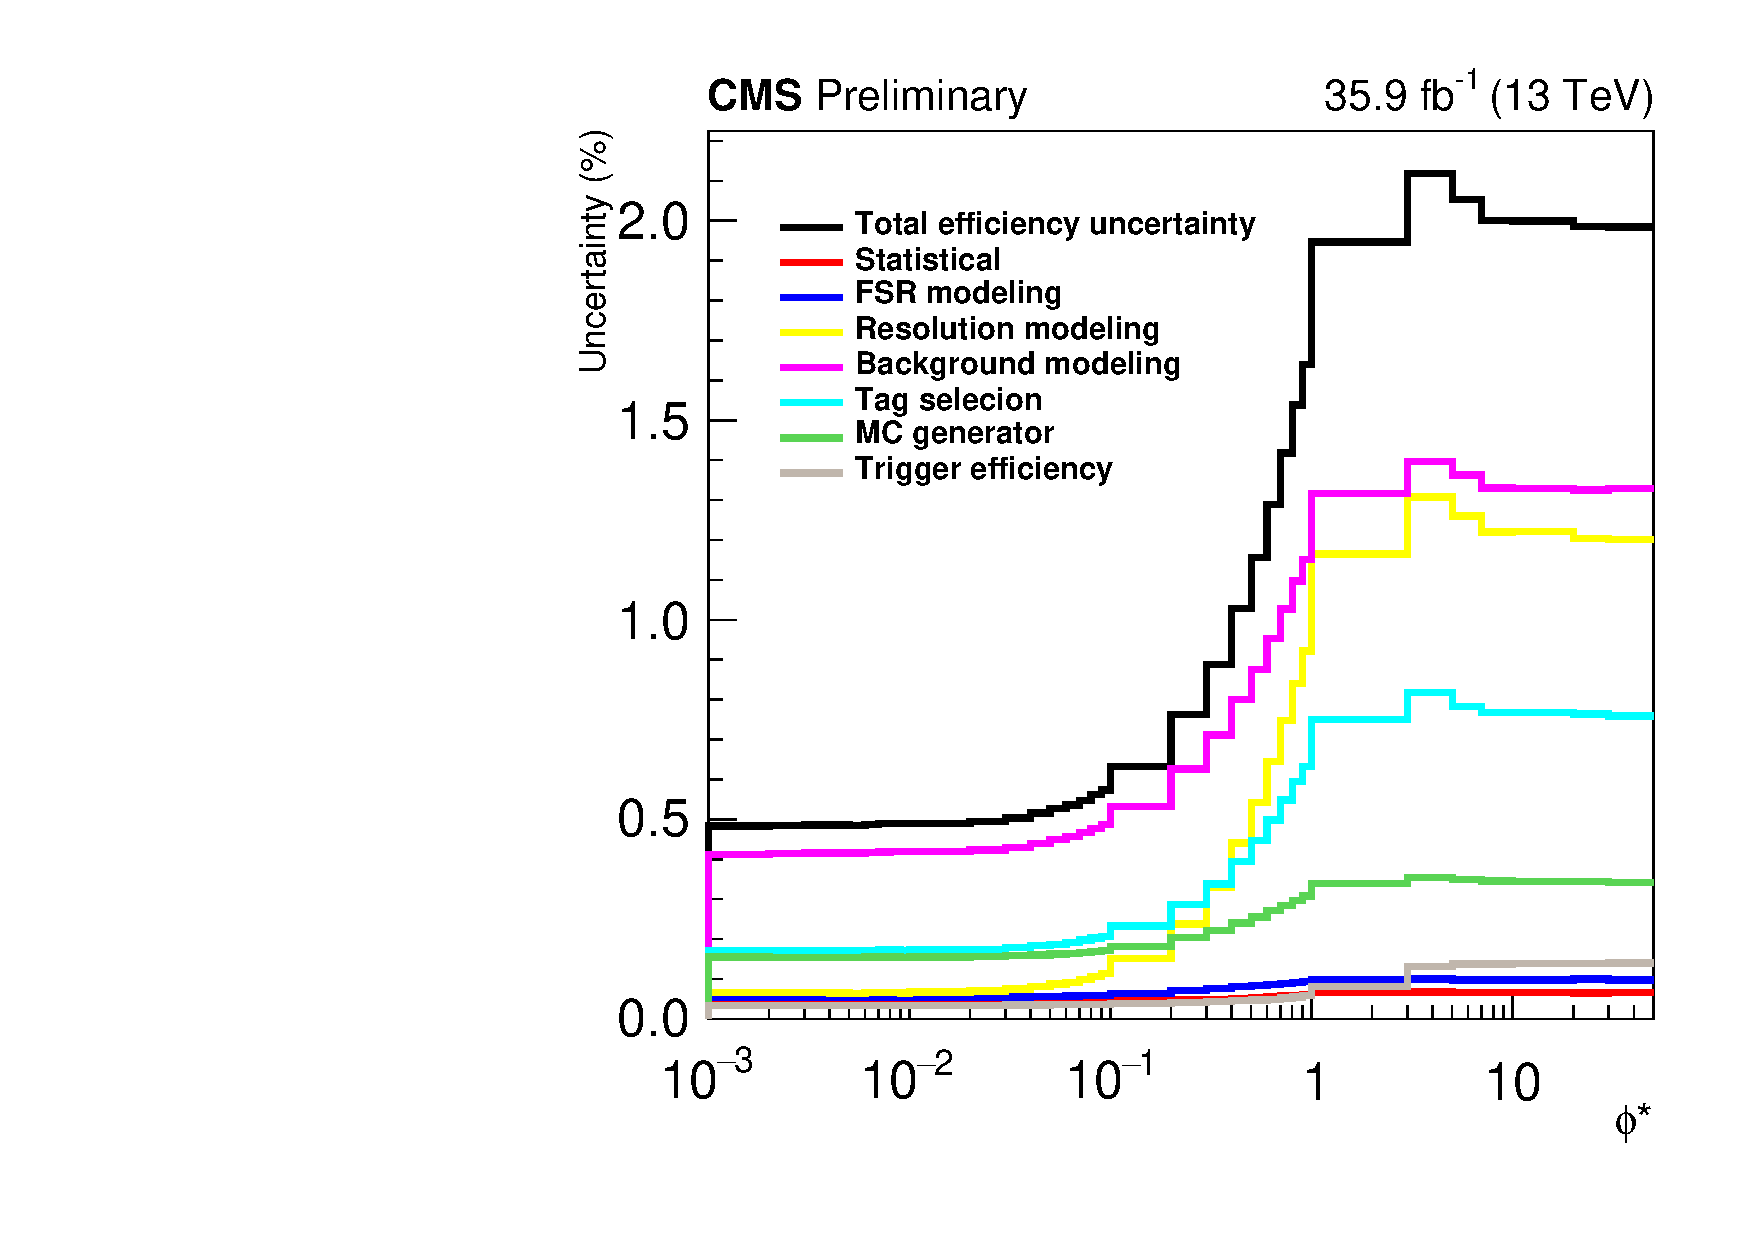
\includegraphics[width=0.49\textwidth]{figures/zpt/histoUnfoldingSystEffPhiStar_nsel0_dy3.pdf}
        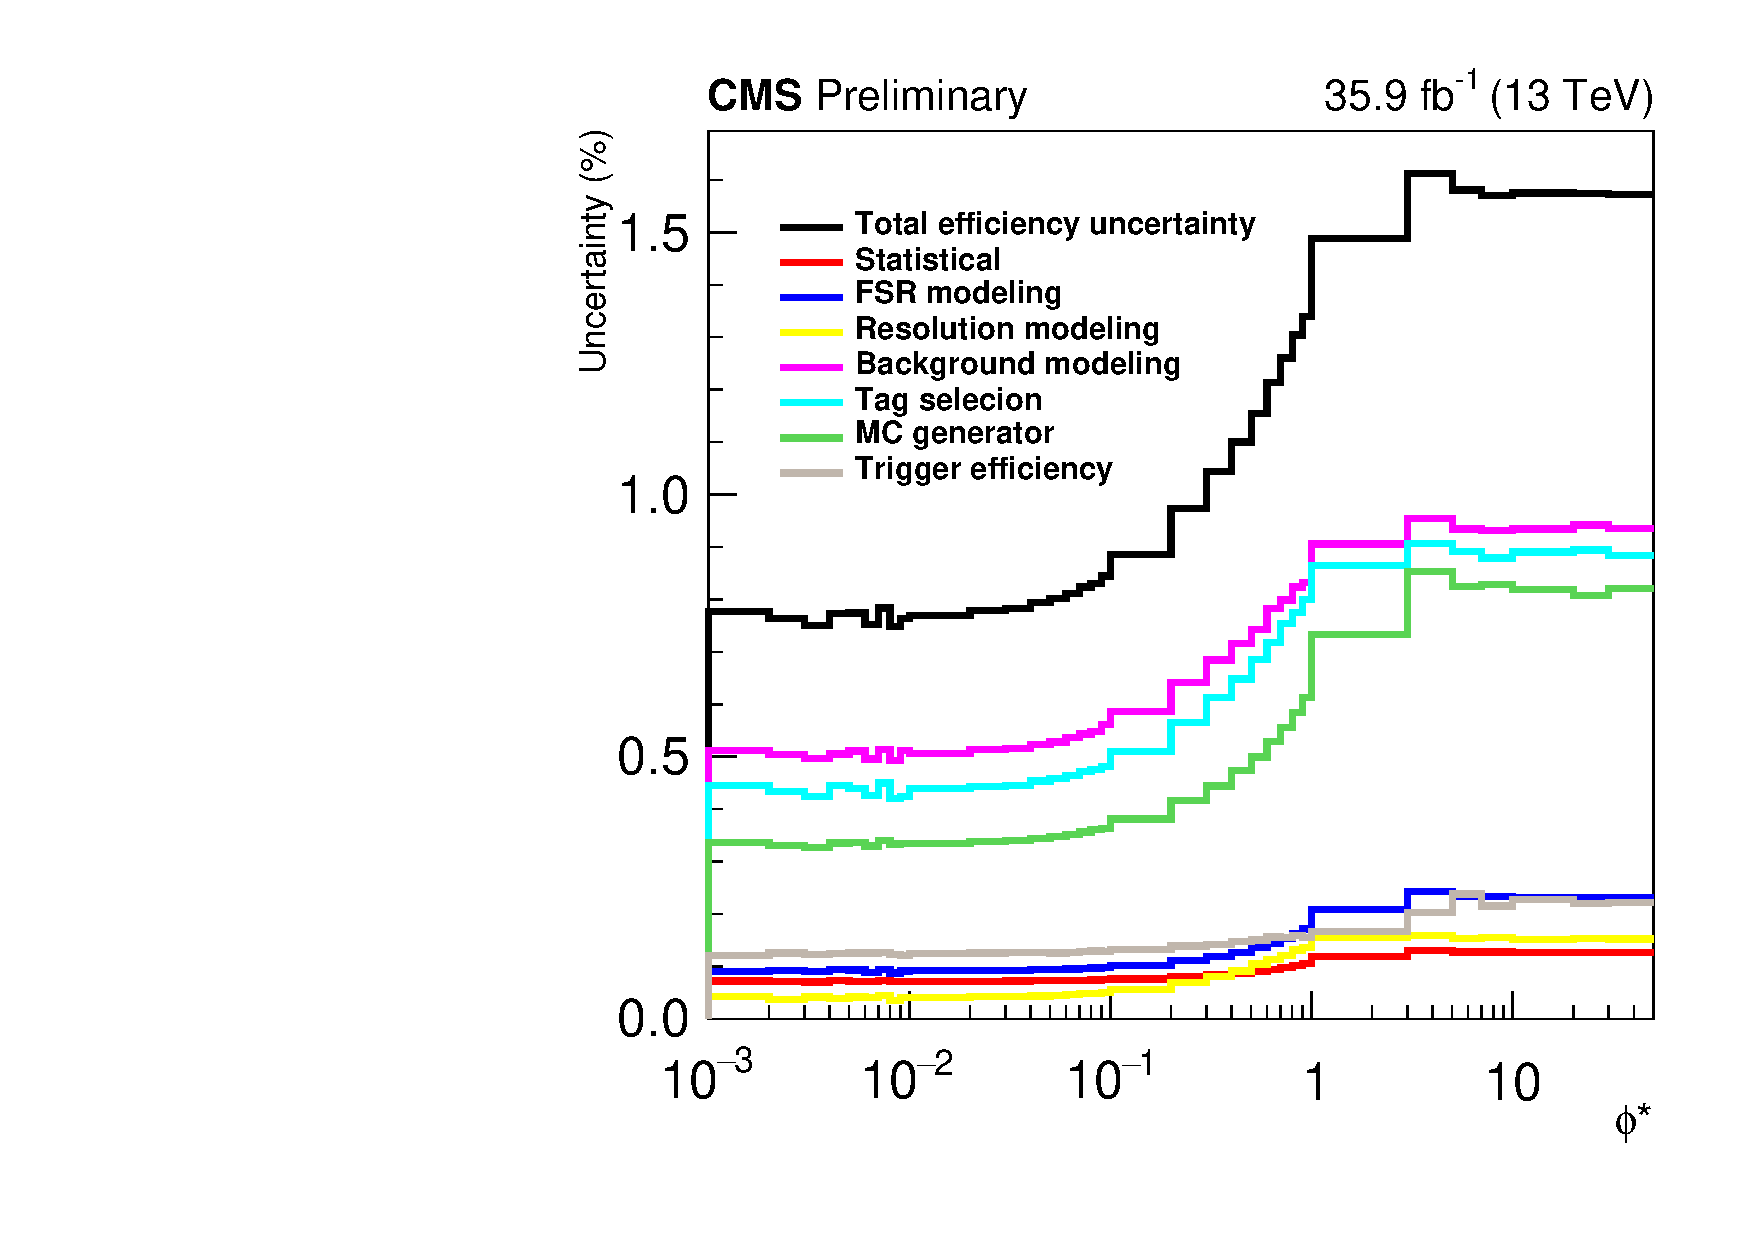
\includegraphics[width=0.49\textwidth]{figures/zpt/histoUnfoldingSystEffPhiStar_nsel1_dy3.pdf}
	\caption{Summary of the systematic uncertainties related to the lepton efficiency measurements of muons (left) and electrons (right) 
	for the $\pt^{\Z}$ analysis (top), the $|\rapidity^\Z|$ analysis (center), and the $\phi^\star$ analysis (bottom).}
	\label{fig:zpt_systeff}
\end{figure}

The differential cross section measurements can also performed with respect to 
the inclusive cross section. Therefore, in that case the uncertainties are 
largely reduced, in particular the lepton reconstruction selection 
efficiency mostly cancel out, and the effect due to the integrated luminosity 
completely cancel out. Those uncertainties are summarized in Figure~\ref{fig:zpt_syst_xratio}.

\begin{figure}
	\centering
	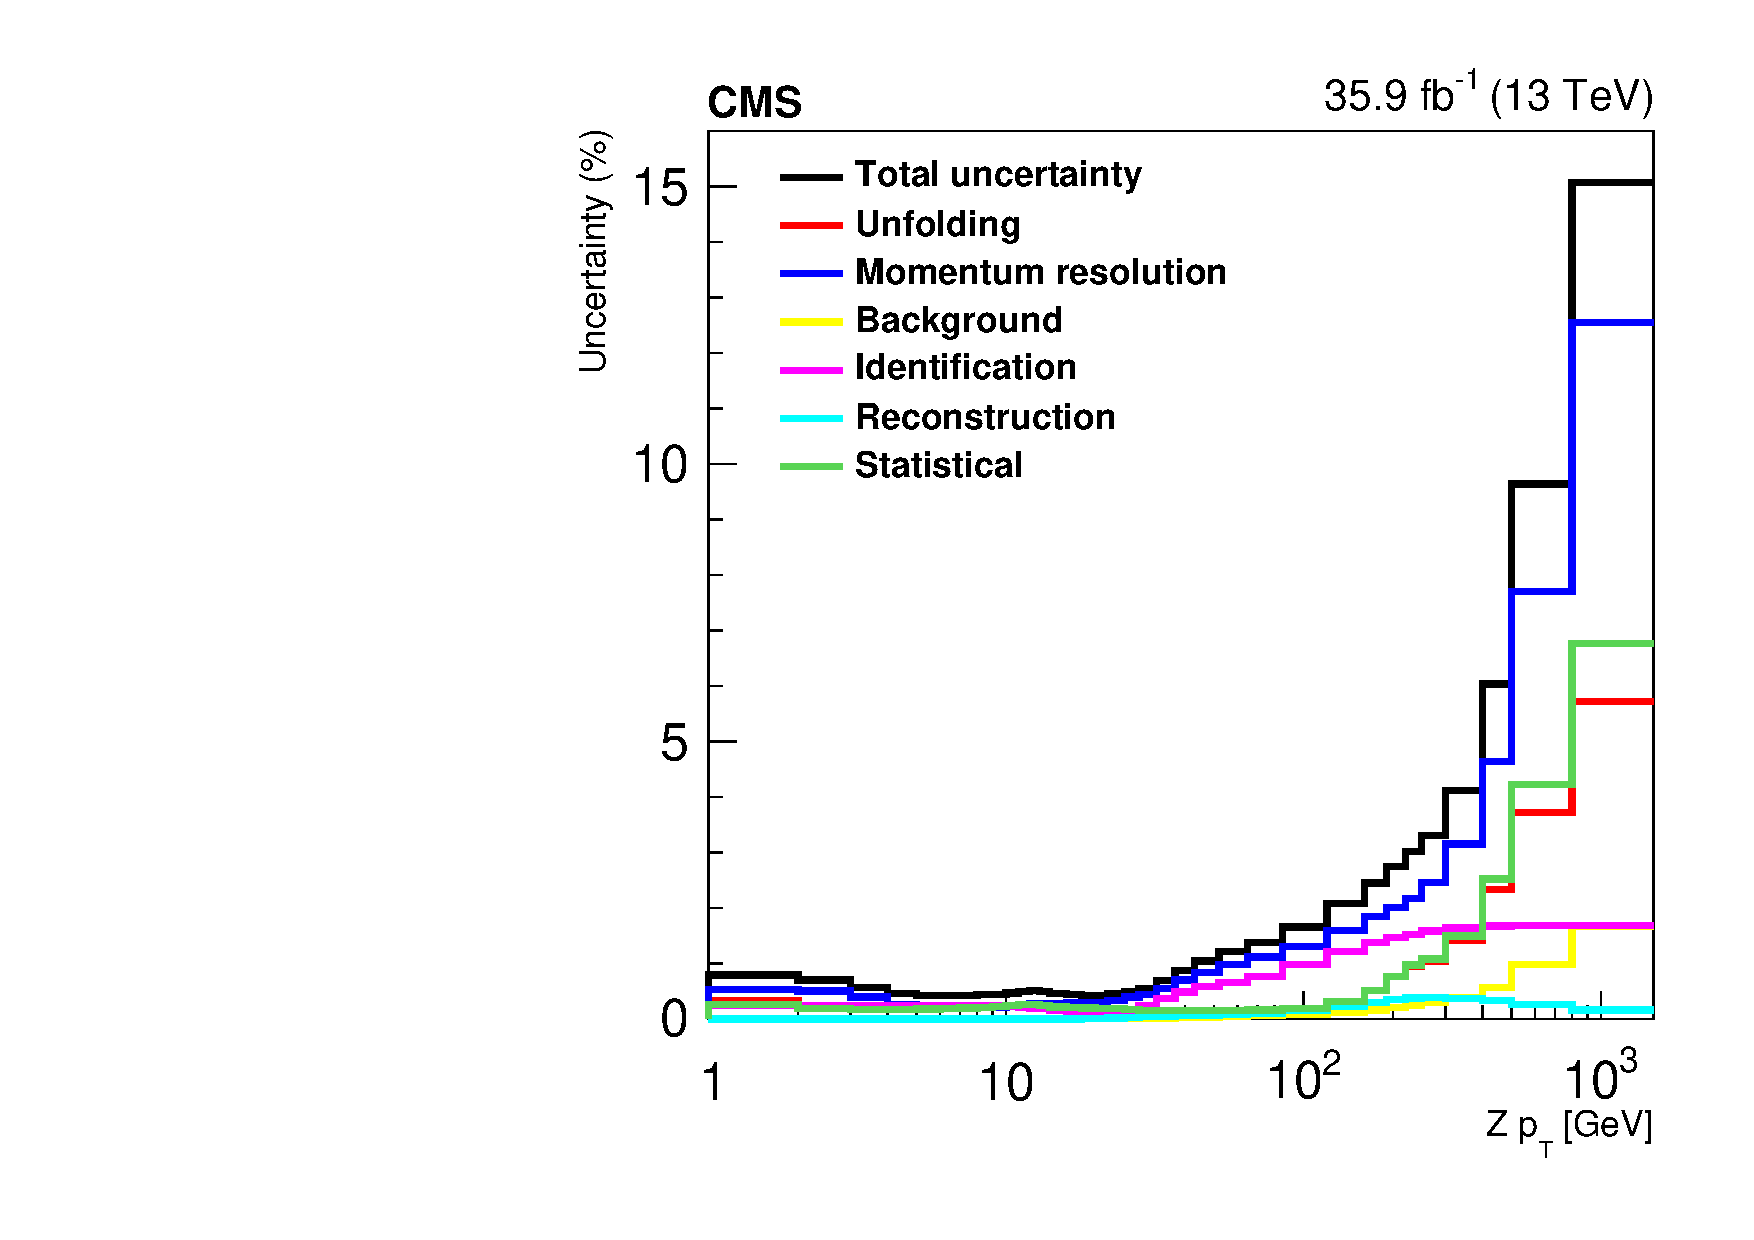
\includegraphics[width=0.49\textwidth]{figures/zpt/histoUnfolding_XSRatioSystPt_nsel0_dy3.pdf}
        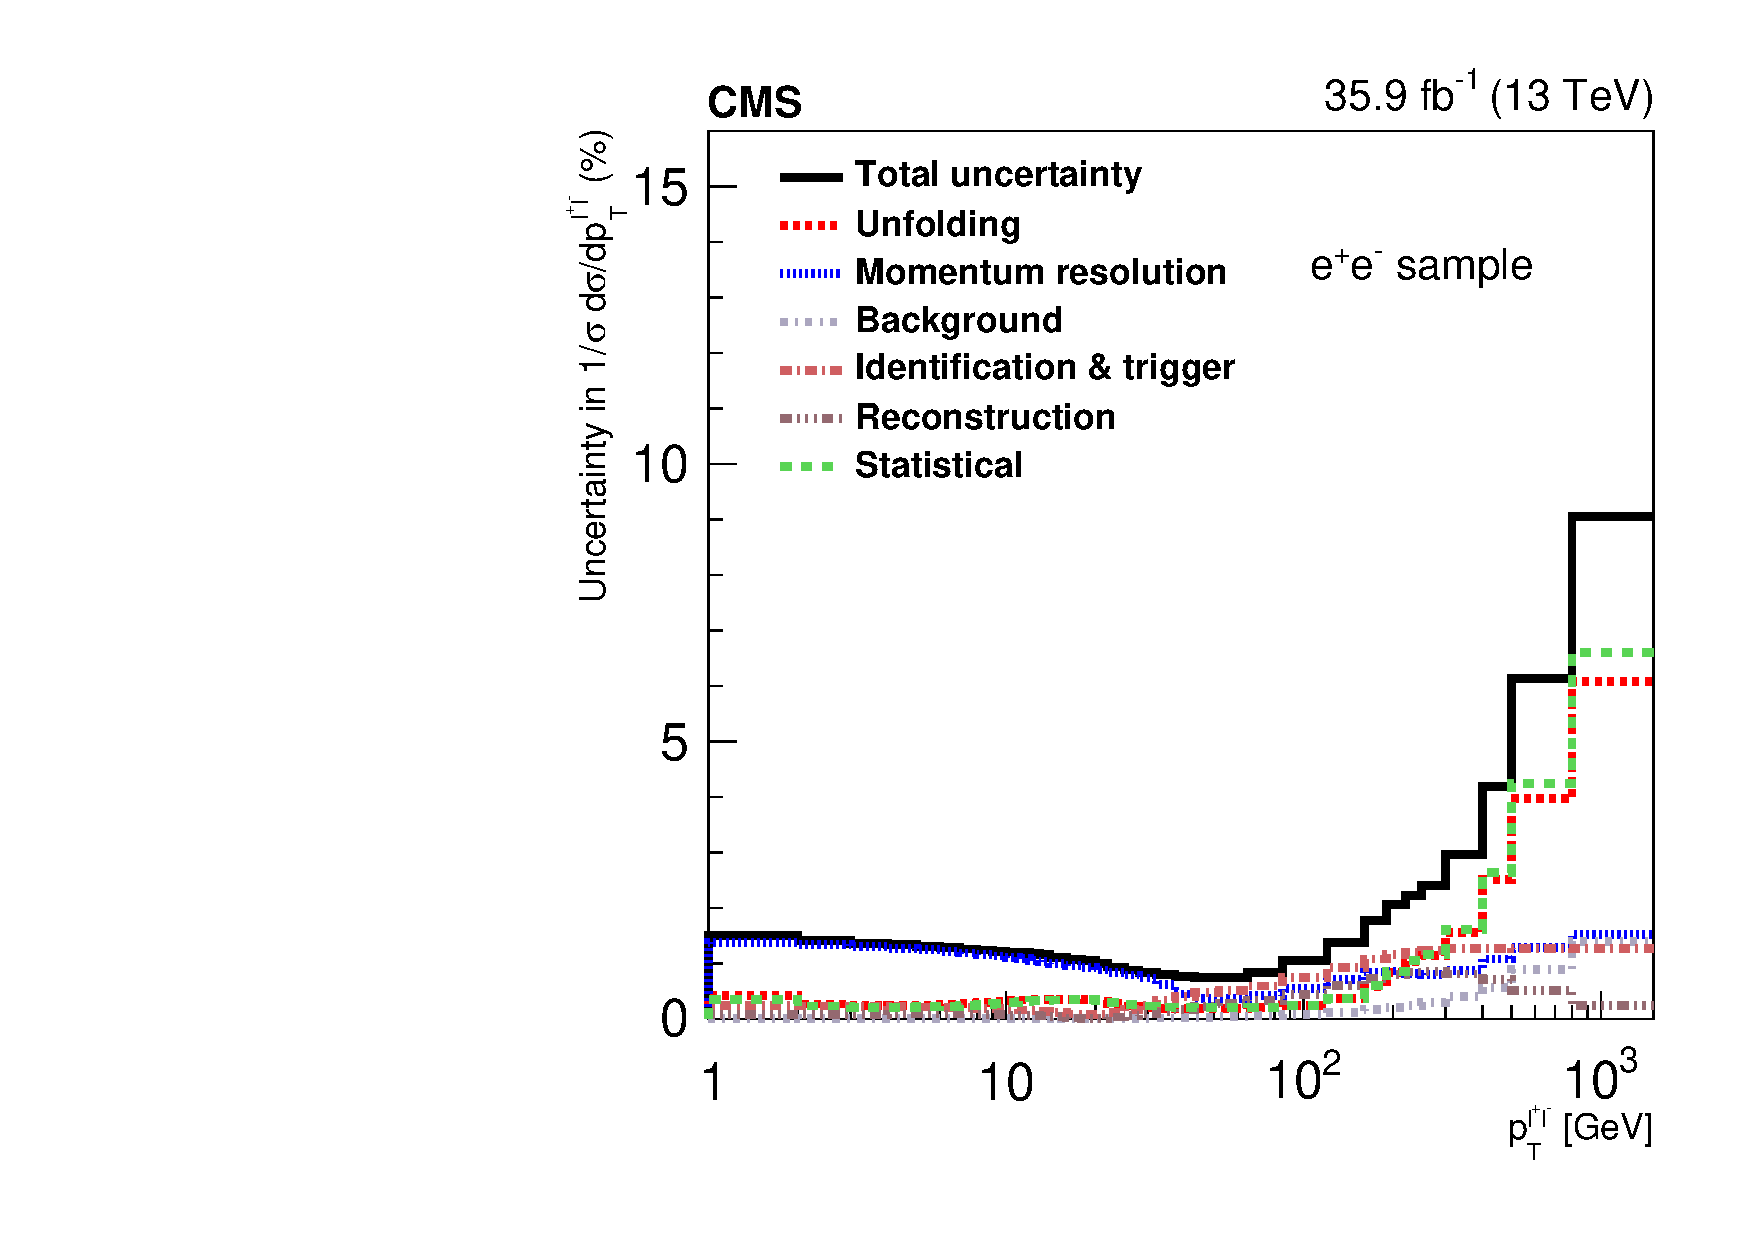
\includegraphics[width=0.49\textwidth]{figures/zpt/histoUnfolding_XSRatioSystPt_nsel1_dy3.pdf}
	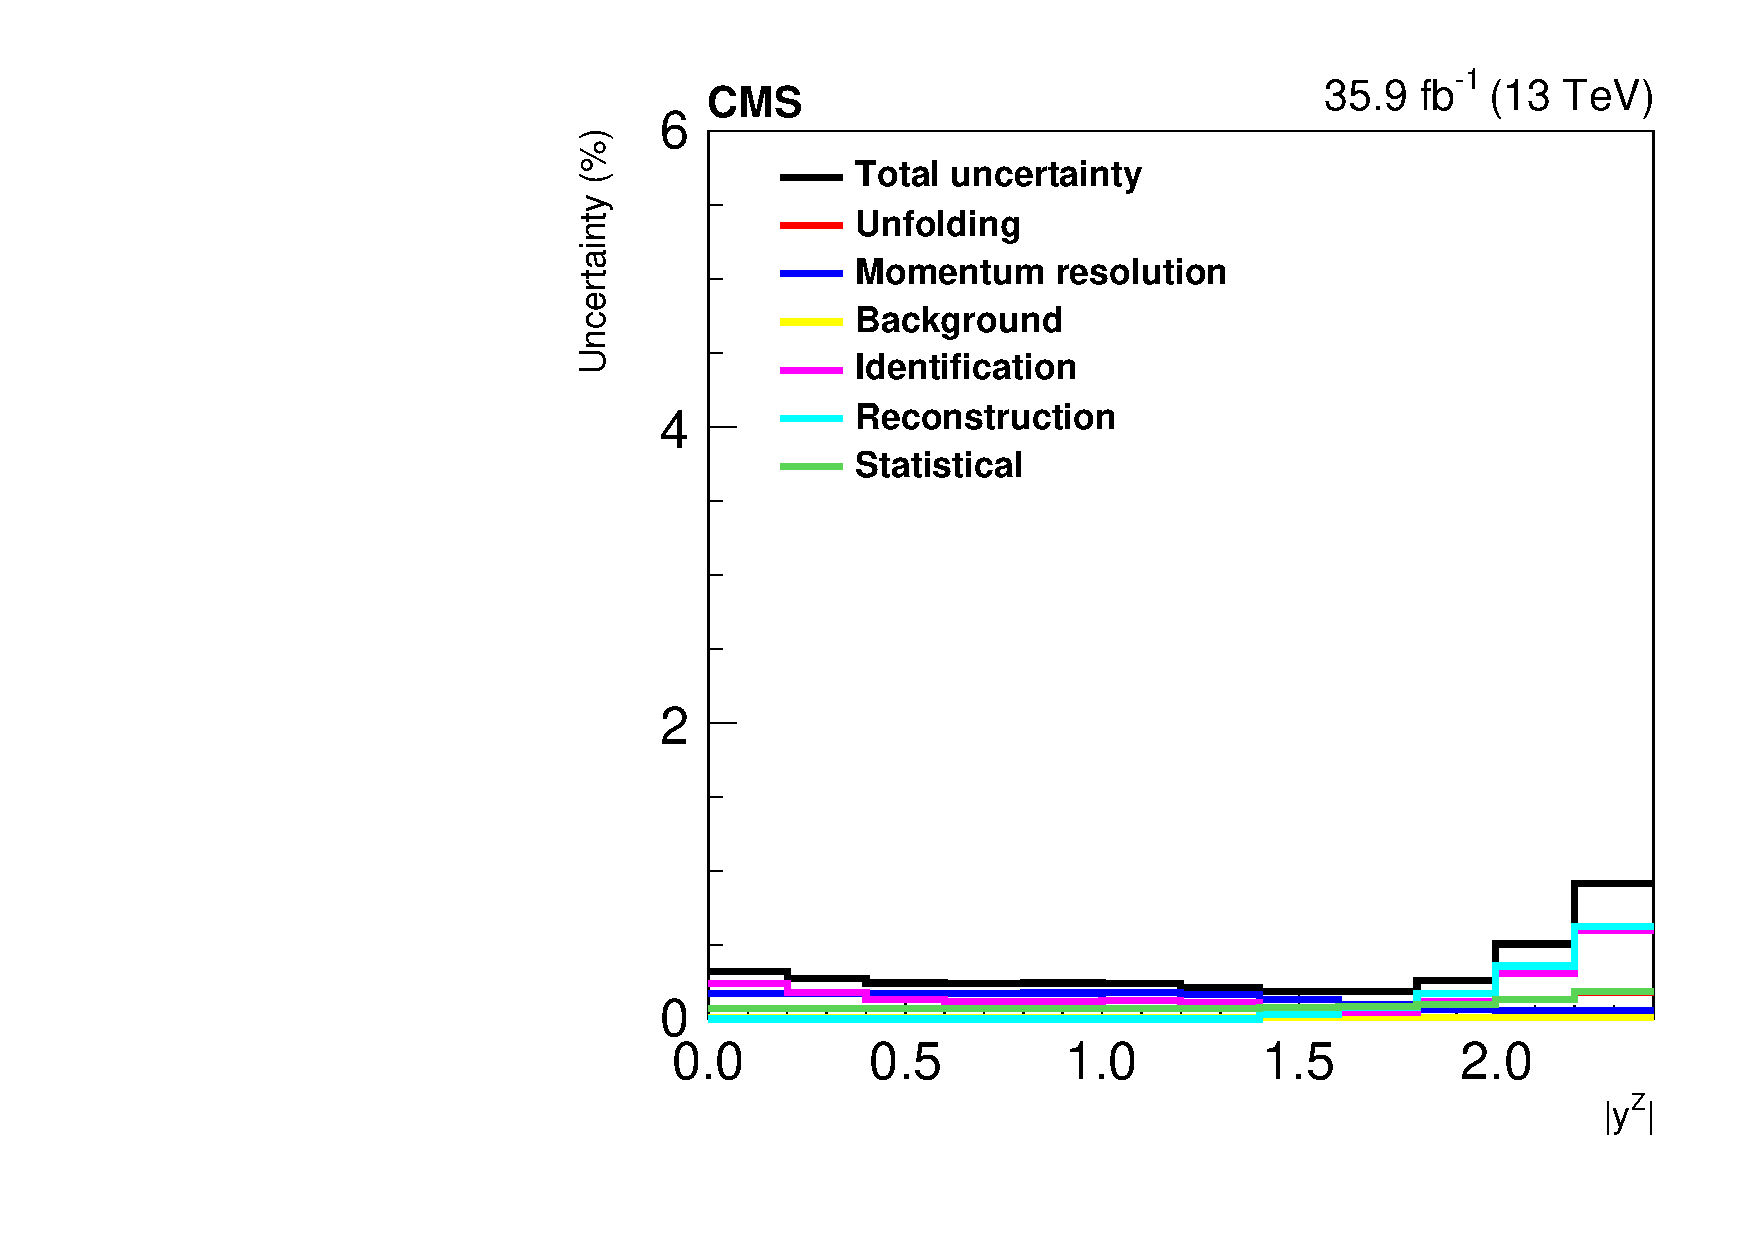
\includegraphics[width=0.49\textwidth]{figures/zpt/histoUnfolding_XSRatioSystRap_nsel0_dy3.pdf}
        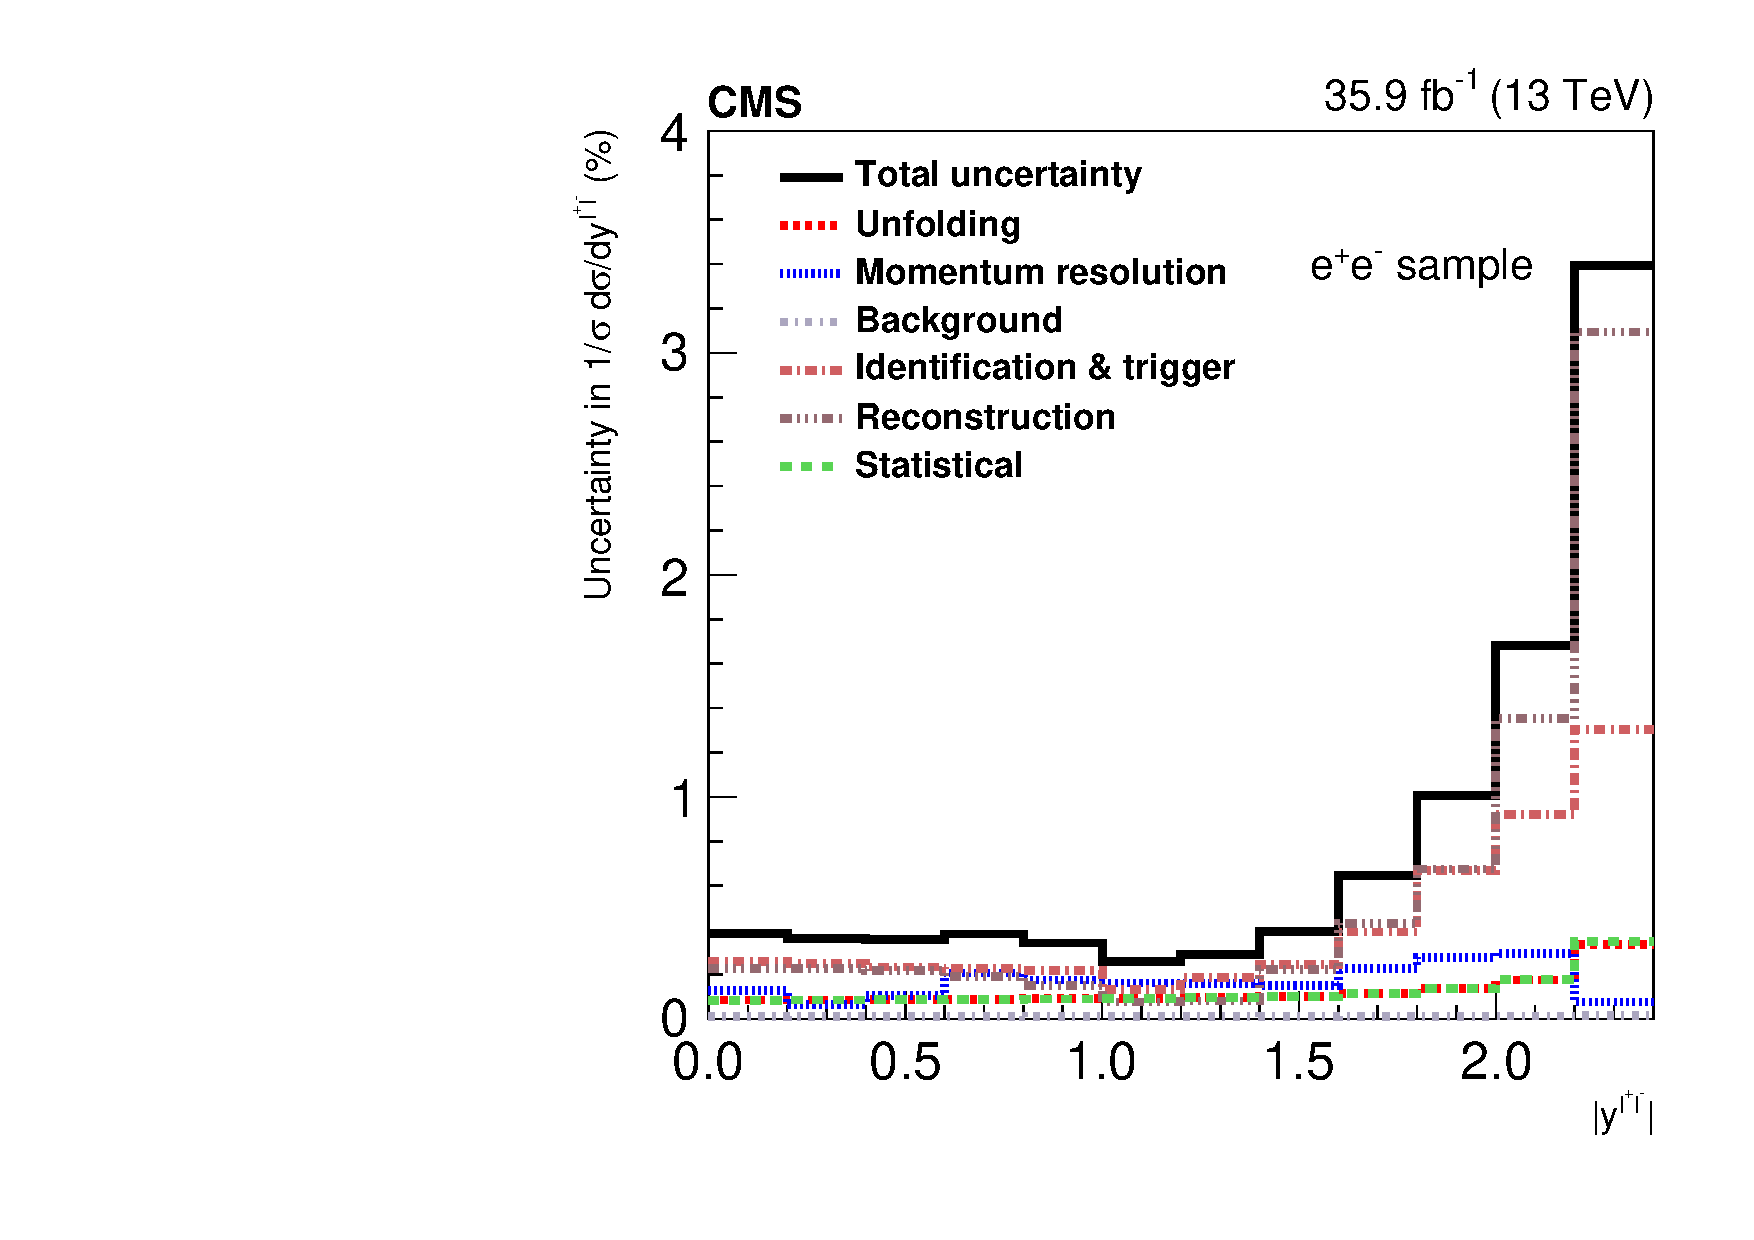
\includegraphics[width=0.49\textwidth]{figures/zpt/histoUnfolding_XSRatioSystRap_nsel1_dy3.pdf}
	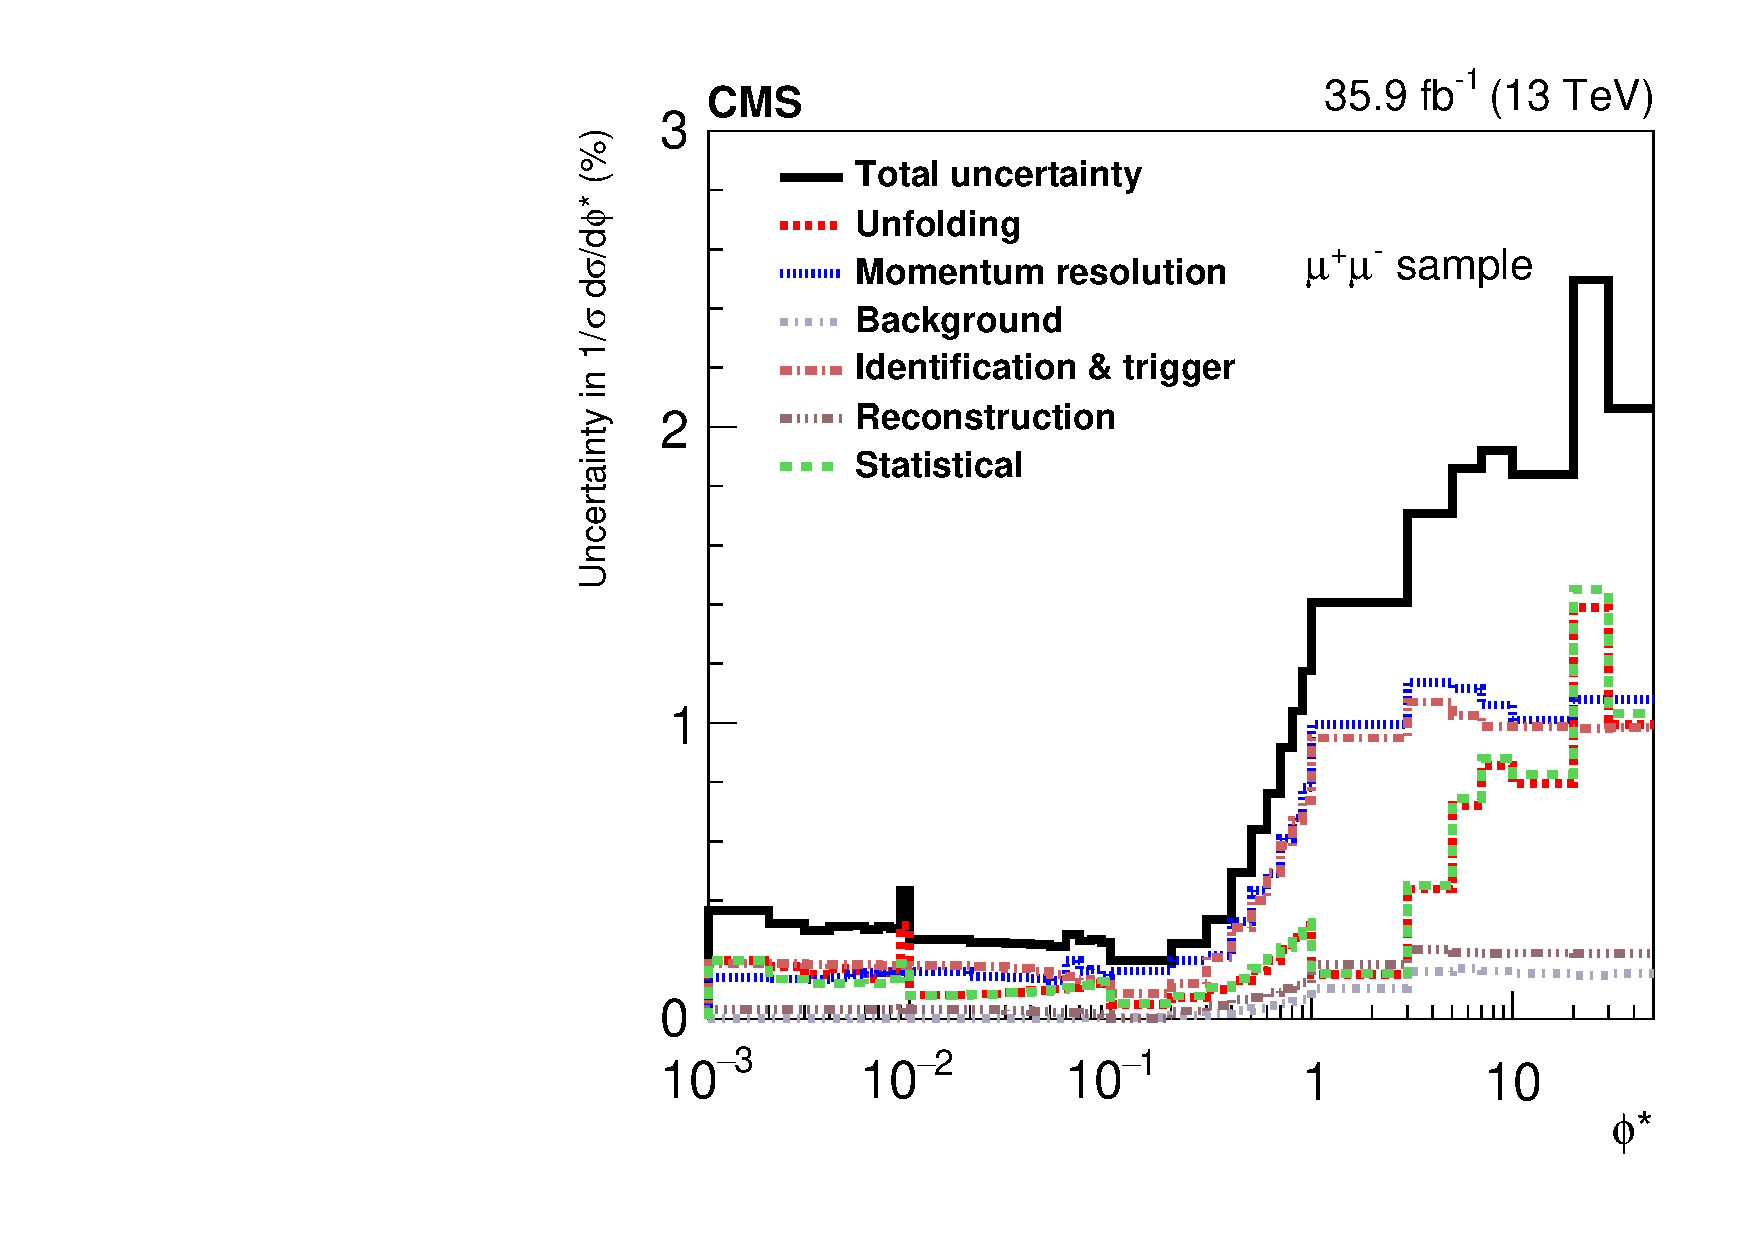
\includegraphics[width=0.49\textwidth]{figures/zpt/histoUnfolding_XSRatioSystPhiStar_nsel0_dy3.pdf}
        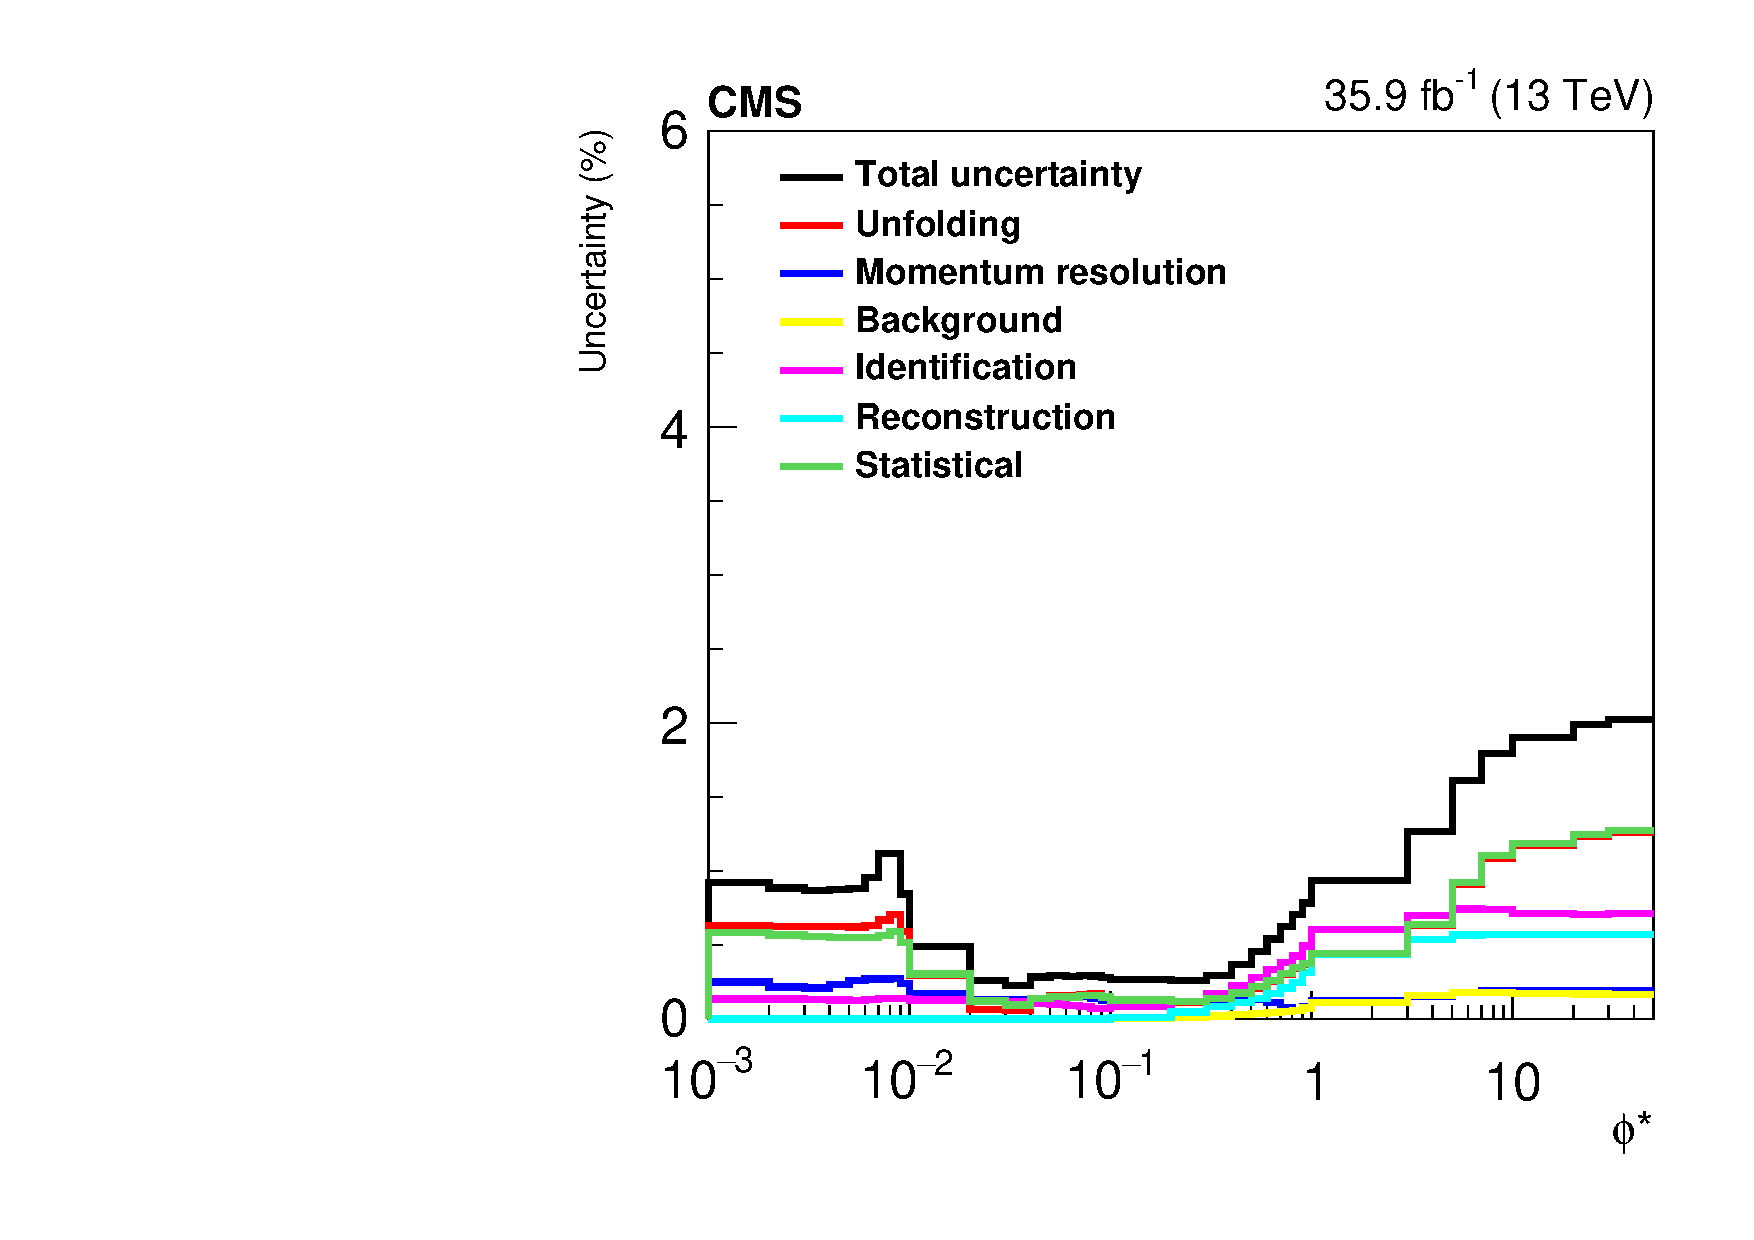
\includegraphics[width=0.49\textwidth]{figures/zpt/histoUnfolding_XSRatioSystPhiStar_nsel1_dy3.pdf}
	\caption{Summary of the systematic uncertainties of muons (left) and electrons (right) 
	for the $\pt^{\Z}$ analysis (top), the $|\rapidity^\Z|$ analysis (center), and the $\phi^\star$ analysis (bottom) 
	for the differential cross section measurements with respect to the inclusive cross section.}
	\label{fig:zpt_syst_xratio}
\end{figure}

\section{Results}
\subsection{Inclusive fiducial cross section measurements}
The inclusive fiducial cross section is measured in the muon-pair and 
electron-pair final states. The combined cross section is obtained by treating 
the systematic uncertainties, except the uncertainties due to the integrated 
luminosity and background estimation, as uncorrelated between the two final states. The luminosity and background estimation uncertainties are treated as fully correlated in the combined measurement. The uncertainties are dominated by the uncertainty in the integrated luminosity and the lepton  efficiency. A summary of the systematic uncertainties is shown in Table~\ref{tab:syst_xs}. The measured cross sections are shown in 
Table~\ref{tab:totCross}. 

\begin{table}[hbtp]
  \begin{center}
\caption{Summary of the systematic uncertainties for the 
inclusive fiducial cross section measurements.\label{tab:syst_xs}}
\begin{tabular}{ccc}
\hline
Source      & $\PZ \to \mu\mu$ (\%) & $\PZ \to \Pe\Pe$ (\%) \\
\hline
Luminosity                         & 2.5     & 2.5     \\
\hline
Muon reconstruction efficiency     & 0.4     &  -      \\
Muon selection efficiency          & 0.7     &  -      \\
Muon momentum scale                & 0.1     &  -      \\
Electron reconstruction efficiency &  -      & 0.9     \\
Electron selection efficiency      &  -      & 0.9     \\
Electron momentum scale            &  -      & 0.2     \\
Background estimation              & $<$ 0.1 & $<$ 0.1 \\
\hline
Total (excluding luminosity)       & 0.8     & 1.3     \\
\hline
  \end{tabular}
  \end{center}
\end{table}


\begin{table}[htb]
\topcaption{
The measured inclusive fiducial cross sections in the muon-pair and electron-pair final states. The combined measurement is also shown.
}
\begin{center}
\begin{tabular}{c|c}
\hline
Cross section                             & $\sigma \, \mathcal{B}$ [pb] \\
\hline
$\sigma_{\PZ \to \mu\mu}$        & $694\pm6\syst\pm17\lum$ \\
$\sigma_{\PZ \to \Pe\Pe}$  & $711\pm9\syst\pm18\lum$\\
$\sigma_{\PZ \to \ell\ell}$       & $699\pm5\syst\pm17\lum$ \\
\hline
\end{tabular}
\label{tab:totCross}
\end{center}
\end{table}


%The measured values are the following
%with respect to the
%theoretical prediction given by \textsc{MadGraph5\_aMC@NLO} are the following
%\begin{itemize}
%  \item[$\sigma_{\PZ \to \mu\mu} =$]   682 $\pm$ 7 (syst.) $\pm$ 17 (lumi.) pb,
%  \item[$\sigma_{\PZ \to \Pe\Pe} =$]   696 $\pm$ 10 (syst.) $\pm$ 17 (lumi.) pb%,
%  \item[$\sigma_{\PZ \to \ell\ell} =$] 686 $\pm$ 5 (syst.) $\pm$ 17 (lumi.) pb.
%\end{itemize}

The measured cross section values agree with the theoretical predictions. The 
predicted values are $\sigma_{\PZ \to \ell\ell} = 682 \pm 55$ pb 
with \textsc{MadGraph5\_aMC@NLO} using the NNPDF 3.0~\cite{nnpdf} NLO PDF set, 
and $\sigma_{\PZ \to \ell\ell} = 719 \pm 8$ pb with fixed order 
FEWZ~\cite{FEWZ, Gavin:2010az, Gavin:2012sy, Li:2012wna} at NNLO accuracy in 
QCD using the NNPDF 3.1~\cite{Ball:2017nwa} NNLO PDF set. The theoretical 
uncertainties for \textsc{MadGraph5\_aMC@NLO} and FEWZ include statistical, 
PDF, and scale uncertainties. The scale uncertainties are estimated by varying 
the renormalization and factorization scales independently up and down by a 
factor of two from their nominal values (removing combinations where both 
variations differ by a factor of four) and taking the largest variations as 
the uncertainty.     

\clearpage
\subsection{Differential cross section measurements}
The measured differential cross sections corrected for detector effects are 
compared to various theoretical predictions. The measured absolute 
cross sections in bins of $|\rapidity^{\PZ}|$ are shown in 
Figure~\ref{fig:unf_rap}. The measurement is compared to predictions using 
parton shower modeling with both \textsc{MadGraph5\_aMC@NLO} and \textsc{POWHEG} at 
NLO accuracy in QCD using the NNPDF 3.0 PDF set. A comparison with fixed order 
prediction at NNLO accuracy with FEWZ using the NNPDF 3.1 NNLO PDF set is also 
shown. The \textsc{MadGraph5\_aMC@NLO} and \textsc{POWHEG} predictions are 
consistent with the data within the theoretical uncertainties. The FEWZ 
prediction with the NNPDF 3.1 PDF set is within 5\% of the measurement over 
the entire $|\rapidity^{\PZ}|$ range.

\begin{figure}
	\centering
        \includegraphics[width=0.45\textwidth]{figures/zpt/zmm_rap.pdf}
	\includegraphics[width=0.45\textwidth]{figures/zpt/zmm_rap_ratio.pdf}
	\includegraphics[width=0.45\textwidth]{figures/zpt/zee_rap.pdf}
	\includegraphics[width=0.45\textwidth]{figures/zpt/zee_rap_ratio.pdf}
	\includegraphics[width=0.45\textwidth]{figures/zpt/zll_rap.pdf}     
	\includegraphics[width=0.45\textwidth]{figures/zpt/zll_rap_ratio.pdf}
	\caption{The measured absolute cross sections (left) in bins of $|\rapidity^{\PZ}|$ for the muon-pair (top) and electron-pair (middle) final states, and for the combination (bottom).  The ratios of the predictions to the data are also shown (right). The shaded band around the data points (black) correspond to the total experimental uncertainty. The measurement is compared to predictions with \textsc{MadGraph5\_aMC@NLO} (square red markers), \textsc{POWHEG} (green triangles), and FEWZ (blue circles). The error bands around the predictions correspond to the statistical, PDF, and scale uncertainties.}
	\label{fig:unf_rap}
\end{figure}

Figure~\ref{fig:unf_pt_shower} shows the measured absolute cross sections in 
bins of $ \pt^{\PZ}$. 
\sloppy{The measurement is compared to predictions using parton shower modeling with \textsc{MadGraph5\_aMC@NLO} and \textsc{POWHEG}.}
A comparison with \textsc{POWHEG} using the \textsc{MiNLO} procedure and using the 
NNPDF 3.1 NLO PDF set is also shown. The predictions are consistent with the 
data within the theoretical uncertainties. The \textsc{POWHEG} predictions at 
high-$\pt$ (above $100~\GeV$) disagree with the data. The higher order 
accuracy of the \textsc{MadGraph5\_aMC@NLO} and \textsc{POWHEG-MiNLO} 
predictions at high-$\pt$ lead to an improved agreement with the data.    

\begin{figure}
	\centering
	\includegraphics[width=0.45\textwidth]{figures/zpt/zmm_shower.pdf}
	\includegraphics[width=0.45\textwidth]{figures/zpt/zmm_shower_ratio.pdf}
	\includegraphics[width=0.45\textwidth]{figures/zpt/zee_shower.pdf}
	\includegraphics[width=0.45\textwidth]{figures/zpt/zee_shower_ratio.pdf}
	\includegraphics[width=0.45\textwidth]{figures/zpt/zll_shower.pdf}
	\includegraphics[width=0.45\textwidth]{figures/zpt/zll_shower_ratio.pdf}
	\caption{The measured absolute cross sections (left) in bins of $\pt^{\PZ}$ for the muon-pair (top) and electron-pair (bottom) final states, and for the combination (bottom). The ratios of the predictions to the data are also shown (right). The shaded band around the data points (black) correspond to the total experimental uncertainty. The measurement is compared to predictions with \textsc{MadGraph5\_aMC@NLO} (square red markers), \textsc{POWHEG} (green triangles), and \textsc{POWHEG-MiNLO} (blue circles). The error bands around the predictions correspond to the statistical, PDF, and scale uncertainties.}
	\label{fig:unf_pt_shower}
\end{figure}

Figure~\ref{fig:unf_pt_fixed} (left) shows comparisons to resummed calculations 
with \textsc{RESBOS}~\cite{Ladinsky:1993zn, Balazs:1997xd, Landry:2002ix} 
and GENEVA~\cite{Alioli:2015toa}. A comparison to 
the \textsc{MadGraph5\_aMC@NLO} prediction is also included as a reference. 
The \textsc{RESBOS} predictions are obtained using the $CP$ version at 
NNLL accuracy with CT14 NNLO PDF set and are consistent with the data within 
the theoretical uncertainties at low-$\pt$ but disagree with the measurements 
at high-$\pt$. The GENEVA predictions include resummation to NNLL accuracy 
where the resulting parton-level events are further combined with parton 
showering and hadronization provided by \textsc{PYTHIA8}. The GENEVA 
predictions are generally consistent with the data within the theoretical 
uncertainties but disagree with the data at low $\pt$ (below $30~\GeV$). 
The CUETP8M1 tune is used for the underlying-event modeling for the shown 
GENEVA predictions. A dedicated tune for the underlying-event modeling will 
lead to improved agreement with the data.  

\begin{figure}
	\centering
	\includegraphics[width=0.49\textwidth]{figures/zpt/zll_ressum_ratio.pdf}
	\includegraphics[width=0.49\textwidth]{figures/zpt/zll_fixed_ratio.pdf}
	\caption{The ratios of the predictions to the data in bins of $\pt^{\PZ}$ for the combination of the muon-pair and electron-pair final states. The shaded band around the data points (black) correspond to the total experimental uncertainty. The left plot shows comparisons to predictions with \textsc{MadGraph5\_aMC@NLO} (square red markers),  Resbos (green triangles), and GENEVA (blue circles). The right plot shows the  $\pt^{\PZ}$ distribution for $\pt>30~\GeV$ compared to predictions with \textsc{MadGraph5\_aMC@NLO} (square red markers),  $\PZ$ + 1 jet at NNLO (green triangles), and FEWZ (blue circles). The error bands around the predictions correspond to the statistical, PDF, and scale uncertainties.}
	\label{fig:unf_pt_fixed}
\end{figure}  

The $\pt^{\PZ}$ distribution for $\pt>30~\GeV$ is compared to fixed order 
predictions as shown in Figure~\ref{fig:unf_pt_fixed} (right). A comparison to 
the \textsc{MadGraph5\_aMC@NLO} prediction is included as a reference. The 
data is compared to the FEWZ predictions at NNLO in QCD and to the complete 
NNLO predictions of vector boson production in association with a 
jet~\cite{Boughezal:2015ded,Boughezal:2015dva}. The central renormalization 
and factorization scale values were chosen to be 
$\mu_{R/F}=\sqrt(P_{TZ}^2+M_{ll}^{2})$ for the FEWZ and $\PZ$+1 jet at NNLO 
predictions. The scale uncertainties are estimated by varying the 
renormalization and factorization scales up and down together within a factor 
of two. The CT14~\cite{Dulat:2015mca} NNLO PDF set is used for the $\PZ$+1 jet 
at NNLO predictions. The predictions are consistent with the data within the 
theoretical uncertainties. As can be seen the $\PZ$+1 jet at NNLO calculations 
significantly reduce the factorization and renormalization scale uncertainties. 
EW corrections are important at high-$\pt$ with correction factors of up to 
$~0.9$ at $\pt=500~\GeV$ and $~0.8$ at 
$\pt=1000~\GeV$~\cite{Dittmaier:2014qza,Lindert:2017olm}. 
The EW corrections are not included in the predictions shown in 
Figure~\ref{fig:unf_pt_fixed}.

%\begin{figure}
%	\centering
%	\includegraphics[width=0.49\textwidth]{figures/zpt/zmm_ressum_ratio.pdf}
%	\includegraphics[width=0.49\textwidth]{figures/zpt/zee_ressum_ratio.pdf}
%	\caption{The ratios of the predictions to the data in bins of $\pt^{\PZ}$ for the muon-pair (left) and electron-pair (right) final states. The shaded band around the data points (black) correspond to the total experimental uncertainty. The measurement is compared to predictions with \textsc{MadGraph5\_aMC@NLO} (square red markers),  Resbos (green triangles), and GENEVA (blue circles). The error bands around the predictions correspond to the statistical, PDF, and scale uncertainties.}
%	\label{fig:unf_pt_ressum}
%\end{figure}

Figure~\ref{fig:unf_phi} shows the measured absolute cross sections in bins 
of $\phi^*$. The measurements is compared to predictions from \textsc{MadGraph5\_aMC@NLO}, \textsc{POWHEG}, and \textsc{POWHEG-MiNLO}. The predictions are consistent with the data within the theoretical uncertainties and describe data well at low $\pt$. 

\begin{figure}
	\centering
	\includegraphics[width=0.45\textwidth]{figures/zpt/zmm_phi.pdf}
	\includegraphics[width=0.45\textwidth]{figures/zpt/zmm_phi_ratio.pdf}
	\includegraphics[width=0.45\textwidth]{figures/zpt/zee_phi.pdf}
	\includegraphics[width=0.45\textwidth]{figures/zpt/zee_phi_ratio.pdf}
	\includegraphics[width=0.45\textwidth]{figures/zpt/zll_phi.pdf}
	\includegraphics[width=0.45\textwidth]{figures/zpt/zll_phi_ratio.pdf}
	\caption{The measured absolute cross sections (left) in bins of $\phi^*$ for the muon-pair (top) and electron-pair (bottom) final states, and for the combination (bottom). The ratios of the predictions to the data are also shown (right). The shaded band around the data points (black) correspond to the total experimental uncertainty. The measurement is compared to predictions with \textsc{MadGraph5\_aMC@NLO} (square red markers), \textsc{POWHEG} (green triangles), and \textsc{POWHEG-MiNLO} (blue circles). The error bands around the predictions correspond to the statistical, PDF, and scale uncertainties.}
	\label{fig:unf_phi}
\end{figure}

Summaries of the absolute double-differential cross section measurements in 
$\pt^{\PZ}$ and $|\rapidity^{\PZ}|$ are shown in Figures~\ref{fig:zll_double0}--\ref{fig:zll_double4}. 
The normalized cross section measurements in bins of  $\pt^{\PZ}$ and  $\phi^*$ are shown in Figure~\ref{fig:cross_norm}. 
The measured normalized cross section  uncertainties are smaller than 0.5\% for $\phi^*<0.5$ and for $\pt^{\PZ}<50~\GeV$. 
Summaries of the normalized double-differential cross section measurements in $\pt^{\PZ}$ and $|\rapidity^{\PZ}|$ are shown in Figures~\ref{fig:zll_norm0}--\ref{fig:zll_norm4}.
The measurements are compared to predictions using parton shower modeling with \textsc{MadGraph5\_aMC@NLO}, \textsc{POWHEG}, and \textsc{POWHEG-MiNLO}. The predictions are consistent with the data within the theoretical uncertainties.     

\begin{figure}
	\centering
	\includegraphics[width=0.47\textwidth]{figures/zpt/zll_double_rap0.pdf}
        \includegraphics[width=0.47\textwidth]{figures/zpt/zll_double_ratio_rap0.pdf}
	\caption{The measured absolute cross sections (left) in bins of $\pt^{\PZ}$ for the $0.0 < |\rapidity^{\PZ}| < 0.4$ region. The ratios of the predictions to the data are also shown (right). The shaded bands around the data points (black) correspond to the total experimental uncertainty. The measurement is compared to the predictions with \textsc{MadGraph5\_aMC@NLO} (square red markers),  $\POWHEG$ (green triangles), and $\POWHEG$-\textsc{MINLO} (blue circles). The error bands around the predictions correspond to the combined statistical, PDF, and scale uncertainties.}
	\label{fig:zll_double0}
\end{figure}

\begin{figure}
	\centering
	\includegraphics[width=0.47\textwidth]{figures/zpt/zll_double_rap1.pdf}
        \includegraphics[width=0.47\textwidth]{figures/zpt/zll_double_ratio_rap1.pdf}
	\caption{The measured absolute cross sections (left) in bins of $\pt^{\PZ}$ for the $0.4 < |\rapidity^{\PZ}| < 0.8$ region. The ratios of the predictions to the data are also shown (right). The shaded bands around the data points (black) correspond to the total experimental uncertainty. The measurement is compared to the predictions with \textsc{MadGraph5\_aMC@NLO} (square red markers),  $\POWHEG$ (green triangles), and $\POWHEG$-\textsc{MINLO} (blue circles). The error bands around the predictions correspond to the combined statistical, PDF, and scale uncertainties.}
	\label{fig:zll_double1}
\end{figure}

\begin{figure}
	\centering
	\includegraphics[width=0.47\textwidth]{figures/zpt/zll_double_rap2.pdf}
        \includegraphics[width=0.47\textwidth]{figures/zpt/zll_double_ratio_rap2.pdf}
	\caption{The measured absolute cross sections (left) in bins of $\pt^{\PZ}$ for the $0.8 < |\rapidity^{\PZ}| < 1.2$ region. The ratios of the predictions to the data are also shown (right). The shaded bands around the data points (black) correspond to the total experimental uncertainty. The measurement is compared to the predictions with \textsc{MadGraph5\_aMC@NLO} (square red markers),  $\POWHEG$ (green triangles), and $\POWHEG$-\textsc{MINLO} (blue circles). The error bands around the predictions correspond to the combined statistical, PDF, and scale uncertainties.}
	\label{fig:zll_double2}
\end{figure}

\begin{figure}
	\centering
	\includegraphics[width=0.47\textwidth]{figures/zpt/zll_double_rap3.pdf}
        \includegraphics[width=0.47\textwidth]{figures/zpt/zll_double_ratio_rap3.pdf}
	\caption{The measured absolute cross sections (left) in bins of $\pt^{\PZ}$ for the $1.2 < |\rapidity^{\PZ}| < 1.6$ region. The ratios of the predictions to the data are also shown (right). The shaded bands around the data points (black) correspond to the total experimental uncertainty. The measurement is compared to the predictions with \textsc{MadGraph5\_aMC@NLO} (square red markers),  $\POWHEG$ (green triangles), and $\POWHEG$-\textsc{MINLO} (blue circles). The error bands around the predictions correspond to the combined statistical, PDF, and scale uncertainties.}
	\label{fig:zll_double3}
\end{figure}

\begin{figure}
	\centering
	\includegraphics[width=0.47\textwidth]{figures/zpt/zll_double_rap4.pdf}
        \includegraphics[width=0.47\textwidth]{figures/zpt/zll_double_ratio_rap4.pdf}
	\caption{The measured absolute cross sections (left) in bins of $\pt^{\PZ}$ for the $1.6 < |\rapidity^{\PZ}| < 2.4$ region. The ratios of the predictions to the data are also shown (right). The shaded bands around the data points (black) correspond to the total experimental uncertainty. The measurement is compared to the predictions with \textsc{MadGraph5\_aMC@NLO} (square red markers),  $\POWHEG$ (green triangles), and $\POWHEG$-\textsc{MINLO} (blue circles). The error bands around the predictions correspond to the combined statistical, PDF, and scale uncertainties.}
	\label{fig:zll_double4}
\end{figure}

\begin{figure}
	\centering
	\includegraphics[width=0.45\textwidth]{figures/zpt/zll_norm.pdf}
        \includegraphics[width=0.45\textwidth]{figures/zpt/zll_ratio_norm.pdf}                      
	\includegraphics[width=0.45\textwidth]{figures/zpt/zll_phi_norm.pdf}
	\includegraphics[width=0.45\textwidth]{figures/zpt/zll_phi_ratio_norm.pdf}
        \includegraphics[width=0.45\textwidth]{figures/zpt/zll_rap_norm.pdf}  
        \includegraphics[width=0.45\textwidth]{figures/zpt/zll_rap_ratio_norm.pdf}    
	\caption{The measured normalized cross sections (left) in bins of $\pt^{\PZ}$ (upper), $\phi^*$ (middle), and $|\rapidity^{\PZ}|$ (lower) for the combined measurement. The ratios of the predictions to the data are also shown (right). The shaded bands around the data points (black) correspond to the total experimental uncertainty. The $\pt^{\PZ}$  and $\phi^*$ measurements are compared to the predictions with \textsc{MadGraph5\_aMC@NLO} (square red markers), $\POWHEG$ (green triangles), and $\POWHEG$-\textsc{MINLO} (blue circles). The $|\rapidity^{\PZ}|$ measurement is compared to the predictions with \textsc{MadGraph5\_aMC@NLO} (square red markers), $\POWHEG$ (green triangles), and $\FEWZ$ (blue circles). The error bars around the predictions correspond to the combined statistical, PDF, and scale uncertainties.}
	\label{fig:cross_norm}
\end{figure}

%\begin{figure}
%	\centering
%	\includegraphics[width=0.45\textwidth]{figures/zpt/zll_double_ratio_rap0.pdf}
%        \includegraphics[width=0.45\textwidth]{figures/zpt/zll_double_ratio_rap1.pdf}
%        \includegraphics[width=0.45\textwidth]{figures/zpt/zll_double_ratio_rap2.pdf}
%        \includegraphics[width=0.45\textwidth]{figures/zpt/zll_double_ratio_rap3.pdf}
%        \includegraphics[width=0.45\textwidth]{figures/zpt/zll_double_ratio_rap4.pdf}
%	\caption{The ratios of the predictions to the data for the combined measurements of the absolute cross sections in bins of $\pt^{\PZ}$ for the 
%	$0.0 < |\rapidity^{\PZ}| < 0.4$ bin (top left), $0.4 < |\rapidity^{\PZ}| < 0.8$ bin (top right),
%	$0.8 < |\rapidity^{\PZ}| < 1.2$ bin (middle left), $1.2 < |\rapidity^{\PZ}| < 1.6$ bin (middle right), and $1.6 < |\rapidity^{\PZ}| < 2.4$ bin (bottom). The measurement is compared to predictions with \textsc{MadGraph5\_aMC@NLO} (square red markers),  \textsc{POWHEG} (green triangles), and \textsc{POWHEG-MiNLO} (blue circles).}
%	\label{fig:zll_double}
%\end{figure}

%\begin{figure}
%	\centering
%	\includegraphics[width=0.45\textwidth]{figures/zpt/zll_ratio_norm.pdf}
%	\includegraphics[width=0.45\textwidth]{figures/zpt/zll_phi_ratio_norm.pdf}
%	\caption{The ratios of the predictions to the data in bins of $\pt^{\PZ}$ (left) and  $\phi^*$ (right) for the combined measurements of the normalized cross sections. The shaded band around the data points (black) correspond to the total experimental uncertainty. The measurement is compared to predictions with \textsc{MadGraph5\_aMC@NLO} (square red markers),  \textsc{POWHEG} (green triangles), and \textsc{POWHEG-MiNLO} (blue circles). The error bands around the predictions correspond to the statistical, PDF, and scale uncertainties.}
%	\label{fig:cross_norm}
%\end{figure}


\begin{figure}
	\centering
	\includegraphics[width=0.45\textwidth]{figures/zpt/zll_double_ratio_normrap0.pdf}
        \includegraphics[width=0.45\textwidth]{figures/zpt/zll_double_ratio_normrap1.pdf}
        \includegraphics[width=0.45\textwidth]{figures/zpt/zll_double_ratio_normrap2.pdf}
        \includegraphics[width=0.45\textwidth]{figures/zpt/zll_double_ratio_normrap3.pdf}
        \includegraphics[width=0.45\textwidth]{figures/zpt/zll_double_ratio_normrap4.pdf}
	\caption{The ratios of the predictions to the data for the combined measurements of the normalized cross sections in bins of $\pt^{\PZ}$ for the 
	$0.0 < |\rapidity^{\PZ}| < 0.4$ bin (top left), $0.4 < |\rapidity^{\PZ}| < 0.8$ bin (top right),
	$0.8 < |\rapidity^{\PZ}| < 1.2$ bin (middle left), $1.2 < |\rapidity^{\PZ}| < 1.6$ bin (middle right), and $1.6 < |\rapidity^{\PZ}| < 2.4$ bin (bottom). The measurement is compared to predictions with \textsc{MadGraph5\_aMC@NLO} (square red markers),  \textsc{POWHEG} (green triangles), and \textsc{POWHEG-MiNLO} (blue circles).}
	\label{fig:zll_double_norm}
\end{figure}

% NEW

\begin{figure}
	\centering
	\includegraphics[width=0.47\textwidth]{figures/zpt/zll_double_normrap0.pdf}
        \includegraphics[width=0.47\textwidth]{figures/zpt/zll_double_ratio_normrap0.pdf}
	\caption{The measured normalized cross sections (left) in bins of $\pt^{\PZ}$ for the $0.0 < |\rapidity^{\PZ}| < 0.4$ region. The ratios of the predictions to the data are also shown (right). The shaded bands around the data points (black) correspond to the total experimental uncertainty. The measurement is compared to the predictions with \textsc{MadGraph5\_aMC@NLO} (square red markers),  $\POWHEG$ (green triangles), and $\POWHEG$-\textsc{MINLO} (blue circles). The error bands around the predictions correspond to the combined statistical, PDF, and scale uncertainties.}
	\label{fig:zll_norm0}
\end{figure}


\begin{figure}
	\centering
	\includegraphics[width=0.47\textwidth]{figures/zpt/zll_double_normrap1.pdf}
        \includegraphics[width=0.47\textwidth]{figures/zpt/zll_double_ratio_normrap1.pdf}
	\caption{The measured normalized cross sections (left) in bins of $\pt^{\PZ}$ for the $0.4 < |\rapidity^{\PZ}| < 0.8$ region. The ratios of the predictions to the data are also shown (right). The shaded bands around the data points (black) correspond to the total experimental uncertainty. The measurement is compared to the predictions with \textsc{MadGraph5\_aMC@NLO} (square red markers),  $\POWHEG$ (green triangles), and $\POWHEG$-\textsc{MINLO} (blue circles). The error bands around the predictions correspond to the combined statistical, PDF, and scale uncertainties.}
	\label{fig:zll_norm1}
\end{figure}


\begin{figure}
	\centering
	\includegraphics[width=0.47\textwidth]{figures/zpt/zll_double_normrap2.pdf}
        \includegraphics[width=0.47\textwidth]{figures/zpt/zll_double_ratio_normrap2.pdf}
	\caption{The measured normalized cross sections (left) in bins of $\pt^{\PZ}$ for the $0.8 < |\rapidity^{\PZ}| < 1.2$ region. The ratios of the predictions to the data are also shown (right). The shaded bands around the data points (black) correspond to the total experimental uncertainty. The measurement is compared to the predictions with \textsc{MadGraph5\_aMC@NLO} (square red markers),  $\POWHEG$ (green triangles), and $\POWHEG$-\textsc{MINLO} (blue circles). The error bands around the predictions correspond to the combined statistical, PDF, and scale uncertainties.}
	\label{fig:zll_norm2}
\end{figure}


\begin{figure}
	\centering
	\includegraphics[width=0.47\textwidth]{figures/zpt/zll_double_normrap3.pdf}
        \includegraphics[width=0.47\textwidth]{figures/zpt/zll_double_ratio_normrap3.pdf}
	\caption{The measured normalized cross sections (left) in bins of $\pt^{\PZ}$ for the $1.2 < |\rapidity^{\PZ}| < 1.6$ region. The ratios of the predictions to the data are also shown (right). The shaded bands around the data points (black) correspond to the total experimental uncertainty. The measurement is compared to the predictions with \textsc{MadGraph5\_aMC@NLO} (square red markers),  $\POWHEG$ (green triangles), and $\POWHEG$-\textsc{MINLO} (blue circles). The error bands around the predictions correspond to the combined statistical, PDF, and scale uncertainties.}
	\label{fig:zll_norm3}
\end{figure}


\begin{figure}
	\centering
	\includegraphics[width=0.47\textwidth]{figures/zpt/zll_double_normrap4.pdf}
        \includegraphics[width=0.47\textwidth]{figures/zpt/zll_double_ratio_normrap4.pdf}
	\caption{The measured normalized cross sections (left) in bins of $\pt^{\PZ}$ for the $1.6 < |\rapidity^{\PZ}| < 2.4$ region. The ratios of the predictions to the data are also shown (right). The shaded bands around the data points (black) correspond to the total experimental uncertainty. The measurement is compared to the predictions with \textsc{MadGraph5\_aMC@NLO} (square red markers),  $\POWHEG$ (green triangles), and $\POWHEG$-\textsc{MINLO} (blue circles). The error bands around the predictions correspond to the combined statistical, PDF, and scale uncertainties.}
	\label{fig:zll_norm4}
\end{figure}

